\documentclass[a4paper,11pt]{scrartcl}
%\usepackage{polyglossia}
%\setdefaultlanguage{english}
\usepackage[T1]{fontenc}
\usepackage[UTF8]{inputenc}
\usepackage[english]{babel}
%\usepackage{csquotes}
%\usepackage{fontspec}
\usepackage{amsmath}
\usepackage{amsfonts}
\usepackage{amssymb}
\usepackage{lmodern}
\usepackage{amstext}
\usepackage{array}
\usepackage{colortbl}
\usepackage{xcolor}
\usepackage{graphicx}
\usepackage{fancyhdr}
\usepackage{pdflscape}
\usepackage{gensymb}
\usepackage{epstopdf}
\usepackage{caption}
\usepackage{calc}
\usepackage[top=2cm, left=1.5cm, right=1.5cm]{geometry}
\usepackage{chemfig, chemmacros}
\usepackage[onehalfspacing]{setspace}
\usepackage{tikz}
\setlength{\parindent}{0pt}
\usepackage{newfloat}
\usepackage{subfigure}
\usepackage{import}
\usepackage{acro}
\usepackage{listings}
\usepackage{float}
\usepackage{morefloats}
\usepackage[version=4]{mhchem}

\acsetup{first-style=short}

\graphicspath{{./Img/}}
\subimport{Abbreviations/}{Abbreviations.tex}

\usepackage[backend=biber,style=chem-angew,sorting=none,maxnames=99,abbreviate=false]{biblatex}

\addbibresource{./Bib/Tutorial.bib}
\newcommand{\myCite}[1]{\textsuperscript{\cite{#1}}}

\clubpenalty = 10000
\widowpenalty = 10000
\displaywidowpenalty = 10000

\begin{document}

\begin{titlepage}
	\begin{titlepage}
		\begin{center}
			\Huge{CAST 3.0}\\
			\Large{Conformational Analysis and Search Tool}\\[.5cm]
			\Huge{Tutorial}\\[1cm]
			
\includegraphics[width=.7\textwidth]{LOGO}\\[1cm]
			\Large{Authors: Daniel Bellinger, Julian Erdmannsdörfer and Dustin Kaiser\\[1cm]
				Last Updated: \today }
		\end{center}
	\end{titlepage}
\end{titlepage}

\setcounter{tocdepth}{4}
\tableofcontents
	
\newpage

\section{About this tutorial}

\section{Getting started: The test molecule}
\label{sec:gettingstarted}

\paragraph{From scratch}First we want to show how to generate TINKER files from scratch. The two programs we will need are molden\myCite{MOLDEN} and tinker. If there is no PDB file of our target molecule available we need to use this procedure to yield a cartesian structure. A very handy program to do so is molden\myCite{MOLDEN}.
\paragraph{Using the editor}Starting molden there is a button called ``ZMAT Editor'' shown in figure \ref{fig:molden} on the very left of the upper images. Pushing this button opens another window with the option to add a line (figure \ref{fig:molden} top middle) which can be clicked to proceed in adding our first atom. The now changed window shows all the atoms in the periodic table. Furthermore next to the section bondlength one can choose whether the added bond is a single, double or triple bond, this only tells molden to use the specific bondlength if molden knows the value. Needless to say that this option will not affect the first atom.
\paragraph{The Molecule}In the following we will create a test molecule which is a small peptide made of Alanine and Glycine. So we start by adding a carbon atom as depicted on the very right of the top row in figure \ref{fig:molden} which makes a red star appear. To proceed a little faster we may want to add a whole substituent so we click on this little star (figure \ref{fig:molden} in the upper middle the very left one). If we successfully pushed the button we see him turning into a sphere (figure \ref{fig:molden} in the middle of the upper middle images). Now we choose the ``Substitute atom by Fragment'' option (figure \ref{fig:molden} in the upper middle the very right) and choose \ce{CH_3}-fragment (figure \ref{fig:molden} on the lower middle row the very left). Now three additional \ce{H}-atoms appear. To go further on we can repeat the actions for substitution to replace one of the hydrogen's with an amine and another hydrogen with a methyl-group. The last hydrogen stays as it is. Unfortunately, molden does not know what we plan to do so it may create distances between atoms which are not very likely. We deal with this issue later on after we have had a closer look at internal coordinates.
\paragraph{Short look at internal coordinates}Now we need another carbon atom which we need to add via the ``Add Line''  option as we did it for the first carbon. In internal coordinates, which we are using to build our peptide, we need for the first atom no spacial information it just lies in space. For the second one we need the distance from the first atom. The third one needs a distance to one of the former ones and an angle defined through the previous ones. As soon as we reach the fourth atom we need as much spacial information as we do in Cartesian-Coordinates which means three values. Let us say the atom we look at is atom $A$, the first value we need is the distance to another atom $B$, the second the angle over atom $B$ to a third atom $C$ and the third value is a torsion between $A$ and a third atom $D$ in respect to the line $B$ and $C$. Of course none of these atoms can be the same atoms so $A\neq B \neq C \neq D$.
\paragraph{Add another atom}While we add another carbon atom the program will ask us for atom $B$ for which we choose our carbon with only four bonds. The next atom $C$ will be the methyl carbon and the last one can be one of the methyl hydrogen atoms. To deal with molden's wrong placements we use our knowledge about internal coordinates and check each atom which is misplaced by clicking on it. In the window showing the internal information the clicked atom is highlighted red as it is marked red in figure \ref{fig:molden} on the lower middle row the right one. Each value can be changed by clicking on the related box and overwriting the old value. If one clicks in the last box all information about bond, angle and torsion partner is revealed. The yellow sphere is atom $B$ its distance to atom $A$ is marked yellow, the green sphere is atom $C$ and the resulting angle is marked green. The light blue sphere is finally atom $D$ and the torsion value is marked light blue. In the case shown in figure \ref{fig:molden} we can not change the torsion of the misplaced hydrogen for it has no torsion because it is just the third atom (see appendix \ref{app:alaglytinker}). But we can change the position of the amine and the carbon by clicking on them and changing their torsion. Now we need to proceed to substitute and add atoms till we got the Ala-Gly-Peptide. If we want to use the \texttt{OPLS-AA}-Force field (FF)- and we will - we got to create a zwitterionic peptide.
\paragraph{Saving as tinker-file}After finishing the structure we click on close to close the Z-Matrix editor and click on write on the main window and choose tinker as output (figure \ref{fig:molden} bottom pictures). We enter the directory and the filename we wish to use and save it. In this case the filename is ``\texttt{AlaGly.xyz}''. Now we have a tinker file with MM3 forcefield parameters changing these to OPLS-AA is desired.
\paragraph{Generating the final tinker-file}The most straight forward way to change the MM3 parameters to ones supported in CAST (like OPLS-AA) is to look inside the tinker file and, for each atom, look up the kind of atom molden has assigned it to. So let's take this little example:

\begin{lstlisting}[frame=single,]
  1  N    -0.679000    1.176000   -0.480000     39   2   6  12  13
\end{lstlisting}

This may be the first atom of the molden generated file. The first integer is the atom number followed by the atom's abbreviation. The three floating point numbers are the x, y and z coordinate values and in the sixth row the atom type is placed. The last integers assign the connected atoms. We need the type and look that up in an MM3 FF file and scroll to the lines beginning with ``atom'' and choose the 39th. The line reads:


\begin{lstlisting}[frame=single,]
atom         39    N+    "NSP3 AMMONIUM"                7    14.003    4
\end{lstlisting}

So now we need a equivalent atom number in the OPLS-AA FF in which are plenty of more atom types as in the MM3 parameter file. So we need to find which atom type this might be. MM3 say ammonium sp3 in OPLS-AA we find:

\begin{lstlisting}[frame=single,]
atom        230   53    N3    "Ammonium RNH3+"               7    14.007    4
\end{lstlisting}

We change the atom type to 230. Changing the atom's abbreviation is optional. The first atom now looks like:

\begin{lstlisting}[frame=single,]
  1  N3    -0.679000    1.176000   -0.480000    230   2  12   6  13
\end{lstlisting}

We need to proceed through the whole molden generated MM3 file and end up with something like the file in appendix \ref{app:alaglytinker}.

\begin{figure}
	\begin{minipage}{\textwidth}
		\centering
		\raisebox{-0.5\height}{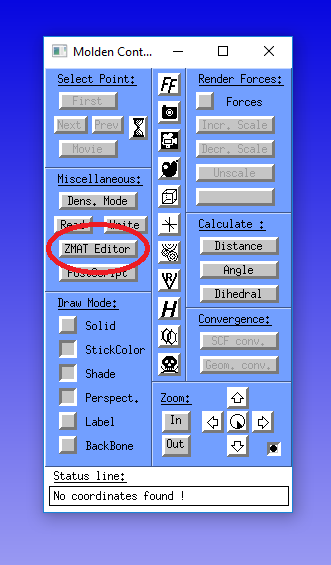
\includegraphics[scale=0.3]{Molden1}}
		\hspace*{.2cm}
		\raisebox{-0.5\height}{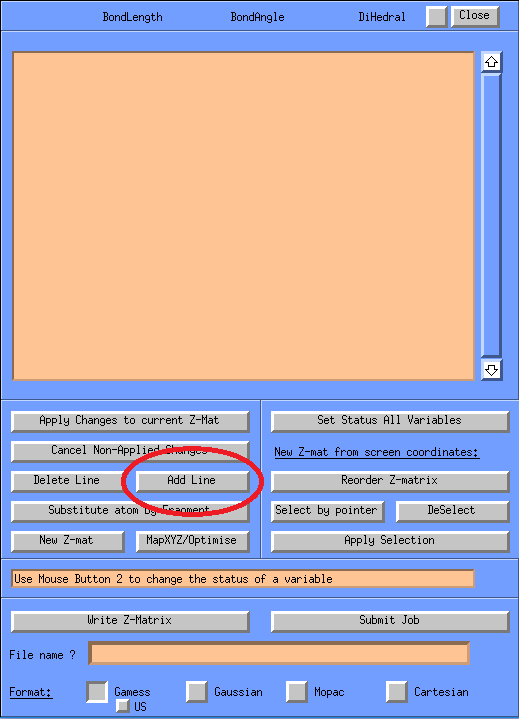
\includegraphics[scale=0.3]{Molden2}}
		\hspace*{.2cm}
		\raisebox{-0.5\height}{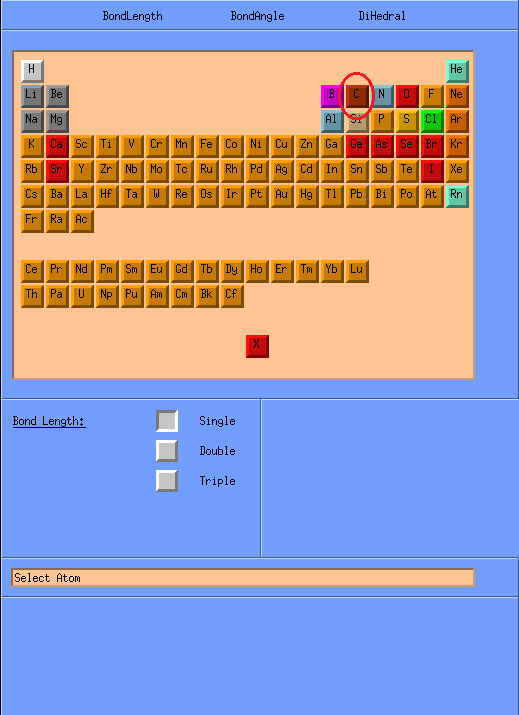
\includegraphics[scale=0.3]{Molden3}}
		\hspace*{.2cm}
		\raisebox{-0.5\height}{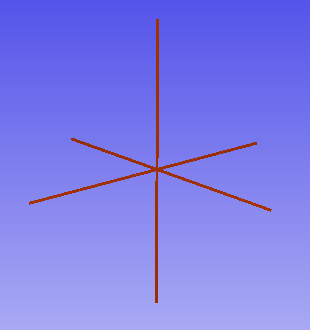
\includegraphics[scale=0.3]{Molden4}}
		\\
		\raisebox{-0.5\height}{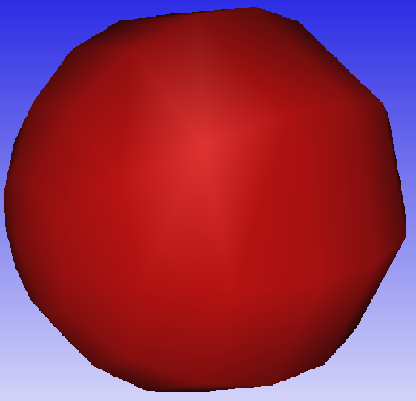
\includegraphics[scale=0.3]{Molden5}}
		\hspace*{.2cm}
		\raisebox{-0.5\height}{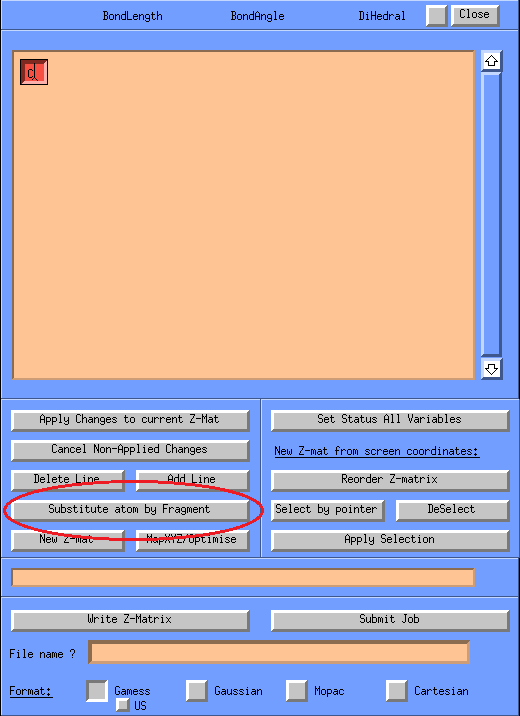
\includegraphics[scale=0.3]{Molden6}}
		\hspace*{.2cm}
		\raisebox{-0.5\height}{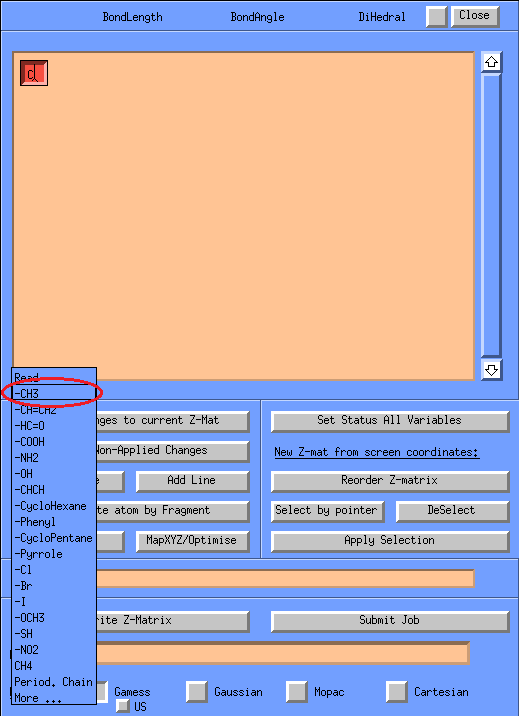
\includegraphics[scale=0.4]{Molden7}}
		\\
		\raisebox{-0.5\height}{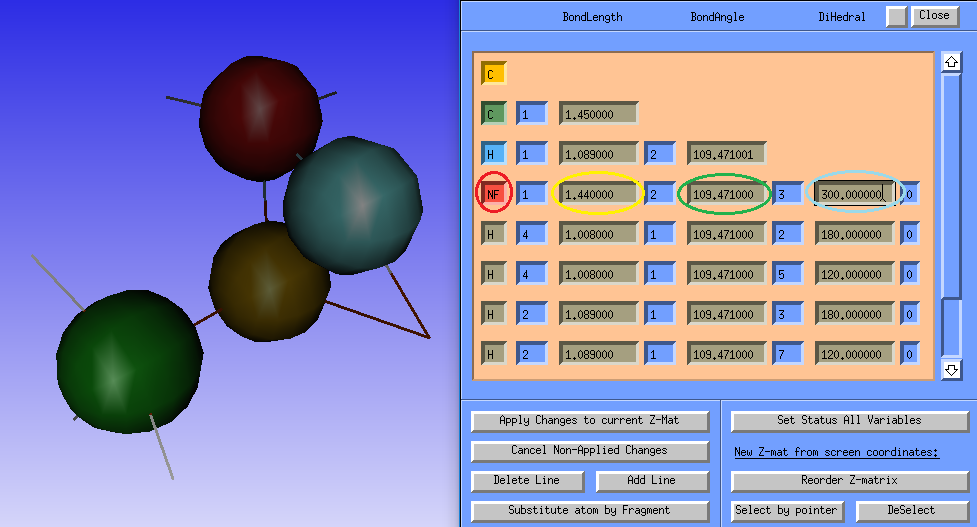
\includegraphics[scale=0.4]{Molden8}}
		\hspace*{.2cm}
		\raisebox{-0.5\height}{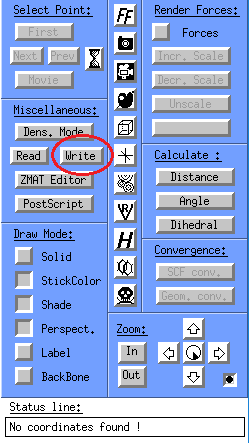
\includegraphics[scale=0.4]{Molden9}}
		\hspace*{.2cm}
		\raisebox{-0.5\height}{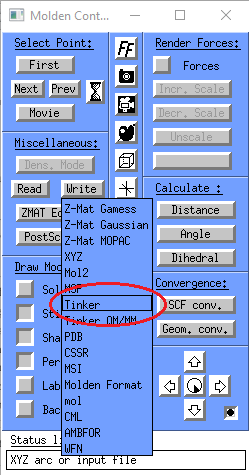
\includegraphics[scale=0.4]{Molden10}}
		\caption{\label{fig:molden} - Molden structure generation process within the "ZMAT Editor"}
	\end{minipage}
\end{figure}

\section{First look at CAST}
\label{sec:firstlook}

Now we are ready to set up the first calculation. The CAST configuration file is shown in appendix \ref{app:casttxt}. This file is part of the downloaded package and is contained in the downloaded main directory. The easiest way is to copy the configuration file directly to the tinker file we want to use otherwise the total path to the file got to be defined in the command prompt by using \texttt{-status="C:\textbackslash{}PATH\textbackslash{}TO\textbackslash{}FILE\textbackslash{}filename.txt"} or \texttt{-s "C:\textbackslash{}PATH\textbackslash{}TO\textbackslash{}FILE\textbackslash{}filename.txt"} after calling CAST. There are two options to start CAST either with a configuration file or using the command prompt alone. Of course one can mix these two possibilities up. In this tutorial we focus on using the configuration file rather than using the second option. There is no particular order in which the configurations in the configuration file are sorted but it is advised to use the predefined configuration file in order to keep things easy. The configuration file is used by giving each keyword a value. In general:

\begin{lstlisting}[frame=single,]
	keyword			value
\end{lstlisting}

Each value for each keyword can be changed to adjust the settings to each respective task which is desired. Let us take a look at the predefined configuration file. The first section contains general settings starting at line \ref{appCAST:castconf} like the amount of information which is printed during the execution which can be changed in line \ref{appCAST:verbosity} by altering the value next to \texttt{verbosity}. Values supported range between 1 (minimal output) and 5 (full debug output - not recomended). The next value, \textit{cores}, sets the number of CPU cores used. Most of the task in CAST are parallelized to some degree, speed-up can be expected. With an \textit{i-X}-Processor there are four cores available and thus the value next to \texttt{cores} in line \ref{appCAST:cores} reads \texttt{4}.\\
The next section is for determining the input and output options beginning at line \ref{appCAST:filestypes} and starting with the name of the molecules file name. In our case we have got to write the name of the Alanine Glycine peptide next to \texttt{name}, so \texttt{AlaGly.xyt} will do. The next option in line \ref{appCAST:output} decides the filename of the final output. In this case we use \texttt{AlaGly\_final}. Some methods automatically name and generate additional output files. As we use a tinker-file as input format we write in line \ref{appCAST:intype} \texttt{TINKER}. Experimental support for AMBER and PDB structures is available but out of the scope of this tutorial. %

At line \ref{appCAST:tasks} in the sample \textit{CAST.txt} file a listing of all possible tasks is shown. The codename of the task we desire has to be written \ref{appCAST:task} next to \texttt{task}. In a first step we want to start a local optimization for which we choose the task \texttt{LOCOPT}. This is the only configuration we can change in this section. The next section concentrates on the energy interfaces \ac{eg} OPLS-AA which we desire to use. To do so we need to write \texttt{OPLS-AA} next to \texttt{interface} in line \ref{appCAST:interface}. We do not need a preinterface (for preoptimization), so we leave the value in line \ref{appCAST:preinterface} unchanged. %
%%%%%%%%%%%%%%%%%%%%%%%%%%%%%%%
%What is a preinterface?
%%%%%%%%%%%%%%%%%%%%%%%%%%%%%%%
The path to the force-field parameter files needs to be adjusted. The desired parameter file needs to be defined in line \ref{appCAST:paramfile}. We change the value to \texttt{OPLS-AA.prm} and copy the FF file to the directory including the \texttt{CAST.txt} and the \texttt{AlaGly.xyz}. Everything is set up for the first optimization; we open a command prompt and enter: 
\begin{lstlisting}[frame=single,]
	cd "C:\PATH\TO\TUTORIAL"
	"C:\PATH\TO\CAST\CAST.exe"
\end{lstlisting}

CAST starts and prints the local optimized structure in the desired outputfile with a \texttt{\_LOCOPT.arc} filename extension. Opening this should yield a file similar to appendix \ref{app:finalarc}.


\section{Available energy interfaces}

CAST includes in principle three different types of energy interfaces. Force fields which are directly included in the CAST code via TINKER-parameter files include the CHARMM, AMBER, OPLS-AA and AMOEBA force fields (FF). In addition to the standard AMOEBA FF, the improved SAPT-FF is included (details will be given in the specific paragraph). The second type are semi-empirical calculations, which are performed via external syscall to the MOPAC program from the Stewart group. The third interface offers the possibility to do DFT calculations on GPUs by using an MPI interface with the Terachem (V1.5) program from Todd Martinez group. Further energy interface are currently being developed.

\paragraph{OPLSAA, AMBER and CHARMM}
CAST includes three standard FFs which possess more or less same functional description, but are different in terms of parametrization. The interface is chosen by the following \texttt{interface} keywords: \texttt{OPLSAA}, \texttt{AMBER}, \texttt{CHARMM}. Besides The interface keyword each of these FFs needs a tinker-parameter file. The keyword is \texttt{paramfile} this is defined in line \ref{appCAST:paramfile} in the example input file. A typical parameter file in Tinker-format looks like:


\begin{lstlisting}[
basicstyle=\footnotesize,
escapeinside={(@*}{*@)},
frame=single,
numbers=left,
]

      ##############################
      ##                          ##
      ##  Force Field Definition  ##
      ##                          ##
      ##############################


forcefield              OPLS-AA

vdwindex                TYPE
vdwtype                 LENNARD-JONES
radiusrule              GEOMETRIC
radiustype              SIGMA
radiussize              DIAMETER
epsilonrule             GEOMETRIC
torsionunit             0.5
vdw-14-scale            2.0
chg-14-scale            2.0
electric                332.06
dielectric              1.0


      #############################
      ##                         ##
      ##  Literature References  ##
      ##                         ##
      #############################


The parameters supplied with TINKER are from "OPLS All-Atom Parameters
for Organic Molecules, Ions, Peptides & Nucleic Acids, July 2008" as
provided by W. L. Jorgensen, Yale University during June 2009. These
parameters are taken from those distributed with BOSS Version 4.8.

Note that "atom type" numbers and not "atom class" numbers are used
to index van der Waals parameters, see the "vdwindex" keyword above

The atom types with (UA) in the description are "united atom" values,
ie, OPLS-UA, where any nonpolar hydrogen atoms are combined onto their
attached atoms. All other parameters are "all-atom", OPLS-AA, including
explicit hydrogen atoms.


      #############################
      ##                         ##
      ##  Atom Type Definitions  ##
      ##                         ##
      #############################


atom          1    1    F     "Fluoride -CH2-F (UA)"         9    18.998    1
atom          2    2    C2    "Fluoride -CH2-F (UA)"         6    14.027    2
atom          3    3    C     "Acetic Acid -COOH (UA)"       6    12.011    3
atom          4    4    O     "Acetic Acid >C=O (UA)"        8    15.999    1
atom          5    5    OH    "Acetic Acid -OH (UA)"         8    15.999    2
atom          6    6    C3    "Acetic Acid CH3- (UA)"        6    15.035    1
atom          7    7    HO    "Acetic Acid -OH (UA)"         1     1.008    1
.....



\end{lstlisting} 

The first block after the FF definition defines several input parameters for the calculations of the potential energy functions like vdw-combination rules and further on.
  

\paragraph{AMOEBA and SAPT-FF - Theoretical Background (optional reading)}
The AMOEBA FF belongs to the class of polarizable FFs. A detailed description can be found in \myCite{Ponder2010}  The SAPT-FF is a specialized kind of the AMOEBA FF, where the short-range electrostatics are treated with a partitioning scheme.
For the description of the electrostatic energy it is a common approach
to use a finite expansion over atomic multipoles. The simple multipole
expansion underestimates the electrostatic energy. For a better
description a penetration energy can be included by using the Coulombic
energy between molecular charge densities. The classical electrostatic
energy (Coulomb) between two molecules A and B is described by the
following expression,
\begin{equation}
E_{es}=\int\int\rho_{A}(r_{A})\rho_{B}(r_{B})|r_{A}-r_{B}|^{-1}dr_{A}dr_{B}\label{eq:Coulombic}
\end{equation}
where $\rho_{A}(r_{A})$ and $\rho_{B}(r_{B})$ are the molecular
charge distributions, containing nuclear and electronic contributions.
In most cases in computational work the electron distribution is approximated
by a set of multipole moments\myCite{Stone1996}. However,
they underestimate the exact energies which can be calculated by exact
integration methods. This is related to the fact that the penetration
of the electronic distribution of molecule A inside molecule B is
not included in these approaches. 

The penetration energy is affected by the Coulomb charge density
between molecular charge distributions (atomic charge distributions),
which means that it is the dominant part. Therefore, the charge distribution
can be split into a sum of atomic and deformation terms. The atomic
charge distributions are described by spherical ones. In consequence
the Coulombic energy is relatively easy to compute. It can be calculated
via functions depending on the distance and several parameters. Then
the contribution term of atom A can be written in the following way\myCite{Spackman1986a},
\begin{equation}
\rho_{A}(r_{A})=\sum_{i\in A}[\rho_{A,i}^{atomic}(r_{A})+\Delta\rho_{A,i}^{elec}(r_{A})]=\rho_{A}^{pro}(r_{A})+\Delta\rho_{A,i}^{elec}(r_{A})
\end{equation}
which describes the partitioning of the molecular electronic distribution.
The molecular charge distribution of spherical atom A is $\rho_{A}^{pro}(r_{A})$
and $\Delta\rho_{A,i}^{elec}(r_{A})$ is the deformation term. Now
it is possible to rewrite $E_{es}$ and fill in $\rho_{A}\rho_{B}$
in eq. \ref{eq:Coulombic} For this $\rho_{A}\rho_{B}$ is shown.
\[
\rho_{A}\rho_{B}=\sum_{i\in A}\sum_{j\in B}[\rho_{A,i}^{atomic}\rho_{B,i}^{atomic}+\rho_{B,j}^{atomic}\Delta\rho_{A,i}^{elec}+\rho_{A,i}^{atomic}\Delta\rho_{B,j}^{elec}+\Delta\rho_{A,i}^{elec}\Delta\rho_{B,j}^{elec}]
\]
\begin{equation}
=\rho_{A}^{pro}\rho_{B}^{pro}+\rho_{A}^{pro}\Delta\rho_{B}^{elec}+\rho_{B}^{pro}\Delta\rho_{A}^{elec}+\Delta\rho_{A}^{elec}+\Delta\rho_{B}^{elec}
\end{equation}
\\
In consequence $E_{es}$ can be expressed in three terms containing
pro molecule and deformation depending energies.
\begin{equation}
E_{es}=E_{pro-pro}+E_{pro-def}+E_{def-def}\label{Ees}
\end{equation}
The description with pseudo atomic spheres leads to zero multipole
moments for the spherical atom. Only the deformation term $E_{def-def}$
includes multipole moments. If no atomic multipole moments are used
all other terms are zero for spherical pseudoatoms, so it is necessary
to use an atomic description. This is the case for the Bader's atoms
in molecules (AIM) theory. There the electronic distribution is divided
into discrete atomic fragments. In the case of fitted charge/multipole
expansions derived from electrostatic potentials it would generally
work, but there are cases for which this approach fails. It is important
to know that there are many differences between the partitioning schemes
and how they are implemented. Especially the multipole expansion and
the convergence criteria can be very different. For instance, AIM
uses a formally infinite expansion, truncated at some level for the
multipole expansion or in the evaluation of the energy. AIM stops
a the hexadecapole level and the energy calculation at $L=l_{A}+l_{B}=8$
(hexadecapole-hexadecapole).

The $E_{pro-pro}$ term in eq. \ref{Ees} describes the Coulomb interaction
between pairs of spherical atomic charge densities. $E_{pro-pro}$
can be the constitutive term in the expression for $E_{es}$ which
is related to the large contribution in the description of an attractive
interaction and is substantial at normal bindings and Van-der-Waals
separations. This energy can be expressed as a function of the distance
between two atomic centers

\begin{equation}
E^{a,b}(R)=\frac{Z_{A}Z_{B}}{R}-\int_{-\infty}^{\infty}\frac{Z_{a}\rho_{b}(r_{2})}{|R_{a}-r_{2}|}dr_{2}-\int_{-\infty}^{\infty}\frac{Z_{b}\rho_{a}(r_{1})}{|R_{b}-r_{1}|}dr_{2}-\int\int_{-\infty}^{\infty}\frac{\rho_{a}(r_{1})\rho_{b}(r_{2})}{|r_{1}-r_{2}|}dr_{1}dr_{2}
\end{equation}
with the nuclear charges $Z$ and the charge distributions $\rho(r)$.
The first term represents the coulomb interactions between two atomic
centers with their charges, the second and the third term represents
the coulomb interaction between the atomic charges and the atomic
charge densities (spherical), and the last term is the interaction
between the charge densities. This three dimensional problem can be
reduced to a one-dimensional integral for integration in reciprocal
space (in atomic units)\myCite{Spackman1986}, 
\begin{equation}
E_{es}^{a,b}=\frac{2}{\pi}\int_{0}^{\infty}[Z_{a}-f_{a}(s)][Z_{b}-f_{b}(s)]j_{0}(sR)ds\label{eq:Spackman E1}
\end{equation}
where $Z_{a}$ is a nuclear charge, $f_{i}(s)$ are the atomic scattering
factors with the scattering vector $s=(4\pi sin\Theta/\lambda)$ and
$j_{o}(sR)$ the spherical Bessel function of zero order\myCite{Tafipolsky2011}.
The atomic scattering factors
\begin{equation}
f_{a}(s)=4\pi\int_{0}^{\infty}\rho_{a}(r)\frac{sin(sr)}{sr}dr
\end{equation}
are obtained from analytical atomic ground state wave functions. The
scattering factors can be expanded with linear combinations of Slater-type
functions. There are a few commonly known possibilities for the ground
state wave function available. For a appropriate description of aromatic
dimers, as noted by Spackman\myCite{Spackman2006}, a contraction scheme
of the hydrogen atom charge density is needed (for the reproduction
of reference data). In consequence to this a description for the contraction
is needed. This can be done by rewriting eq. \ref{eq:Spackman E1}
and obtain
\begin{equation}
E_{es}^{a,b}=\frac{2}{\pi}\int_{0}^{\infty}[Z_{a}-f_{a}(s)/\kappa_{a}][Z_{b}-f_{b}(s)/\kappa_{b}]j_{0}(sR)ds\label{Spackman E2}
\end{equation}
where $\kappa_{a}$ and $\kappa_{b}$ are contraction parameters for
the charge densities of atoms $a$ and $b$. In the original paper
of Spackman \myCite{Spackman2006} this contraction parameter has been
set to the value of 1. If $\kappa>1$ then a contraction is the result
and if $\kappa<1$ an expansion is realized. The integral in eq. \ref{Spackman E2}
can be solved numerically by a one dimensional numerical strategy.

The $E_{pro-def}$ term in eq. \ref{Ees} characterizes the interaction
between the charge density of one molecule and the atomic deformation
term in another. This term is very small and only notable for small
separations between atoms. For dimers of small molecules the energy
is always positive and in the range of 1.5 kJ/mol. In conclusion,
it can be said that $E_{pro-pro}$ is one of the most important terms
for the electrostatic energy description and is called the \textbf{Spackman-correction}
in this work. The deformation energy $E_{def-def}$ is one of
the key terms in the description of intermolecular interactions. For
this term the description depends on the used force field or the used
multipole moments (for example DMA multipoles).

\paragraph{How to run a SAPT-FF/AMOEBA calculation}

For running an AMOEBA or the SAPT-FF calculation the \texttt{interface} keyword should be set to \texttt{AMOEBA}. The SAPT-FF is activated by using the \texttt{Spackman} keyword (see line \ref{appCAST:mopacpath}). This keywords needs three input parameters: activation (0/1), interpolated gradients (0/1) and cutoff radius for the elect. interactions (standard=10.0).

\textbf{Spackman} 1 1 10.0 - short-range correction activated, interpolative calculation activated and cutoff is set to 10.0 $\AA$

The SAPT-FF calculation needs several additional input files. At the evry least CAST needs the Spackman.prm file which contains the $\kappa$ and the atomic basis information. If one would like to use the interpolative variant, the precalculated energy and gradient lists are needed. These files are called XY\_EN.in or XY\_GRAD.in. For a successful calculation one needs all the .in files (at the moment 20 files, included in the CAST package). The Spackman.prm file is given in the appendix (see line \ref{appCAST:spackman}). Within the parameter files the $\kappa$ values can be changed (see line \ref{appCAST:spackmankappa}. The first number indicates the atom type by the atomic charge value.


\paragraph{MOPAC}

In order to use the \texttt{MOPAC} energy interface one needs to install the latest Version of MOPAC (MOPAC2012/16) to do calculations. For academic groups MOPAC can be freely downloaded from: \textit{http://openmopac.net/downloads.html}. The MOPAC interface is an file I/O interface and needs some input parameters to generate the appropriate input file. Generally the MOPAC interface can be combined with all existing tasks which need an energy or gradient evaluation. The most important keywords are:
 
\begin{itemize}
\item \textbf{MOPACpath} \textit{Character String} - defines the absolute pathway to the binary installed on the system 

\item \textbf{MOPACkey} \textit{Character String} - delivers the essential input parameters like method (standard = PM7)

\item \textbf{MOPACdelete} \textit{bool} - decision about saving or deleting temporarily generated files

\end{itemize}

\paragraph{TERACHEM}

TeraChem is accessed via MPI when the keyword \glqq TERACHEM\grqq~is specified in the energy interface. All further parameters regarding basis set, functional and so on have to be set in an extra file readable by CAST. CAST then transfers the input parameters to TeraChem via MPI. The syntax for the TeraChem input is such that each string needs to be set in its own line. Otherwise it's identical to the TeraChem input. An example is shown below:
		
\begin{lstlisting}[frame=single,]
basis
cc-pvdz
charge
0
method
b3lyp
dftgrid
2
dftd
d2\end{lstlisting}

The name for the TeraChem input has to be \glqq \textit{CAST\_TERACHEM\_OPTIONS.txt}\grqq.
Currently, only TeraChem Version 1.5K is supported. TeraChem has to be started with the \textit{-UseMPI} command line switch.

\newpage

\section{Tasks avaibale in CAST - a walkthrough}

\paragraph{SP}We may compare the total energy of our ``initial guess'' and the local minimum we found earlier. To do so we can look at the \texttt{AlaGly\_final\_LOCOPT.txt} file to obtain the energy of the local minimum which reads $-125.525~kcal/mol$. So we can compute the energy of the initial guess by doing a \ac{sp} calculation (via changing the task keyword to \texttt{SP}). Remember, the task was in line \ref{appCAST:task} in the input file seen in appendix \ref{app:casttxt}. We change the task and run CAST again.

\begin{lstlisting}[frame=single,]
cd "C:\PATH\TO\TUTORIAL"
"C:\PATH\TO\CAST\CAST.exe"
\end{lstlisting} 

We obtain a total energy of $5.204~kcal/mol$ for the initial guess. The same way one could calculate the gradients by using the keyword \texttt{GRAD}.

\paragraph{MD}%In a local minimum a \ac{md} simulation should do pretty bad because the gradient's value should be very close to zero. But nevertheless after some simulation time something may should happen. So we may rather use the not optimized file.
A \ac{md} simulation describes the behavior of an ensemble of particles during a period of time by integrating over the classical Newton laws of mechanics. To use CAST to do so we take a closer look at the input file in appendix \ref{app:casttxt}. 
The configuration options for \ac{md} starts at line \ref{appCAST:md}. A few lines below we see the \texttt{MDsteps} option in line \ref{appCAST:mdsteps}. We can use this to assign the value of how many steps we want to perform. The number of steps should be chosen in relation to the size of the time step. Keep in mind that a \ac{md} simulation needs very small time steps to yield accurate results. We set the step number to \texttt{50000}. The \texttt{MDintegrater} option in line \ref{appCAST:mdintegrator} lets us choose which integrator we want to use. We can choose between the Velocity-Verlet\myCite{VelVer} implementation and the Beeman\myCite{Beeman} one. Let's use the Velocity-Verlet one known from basic computational chemistry textbooks. The \texttt{MDveloscale} option in line \ref{appCAST:mdveloscale} is set to one. A thermostat would be nice to observe \ac{md} on one specific temperature so we choose for \texttt{MDthermostat} in line \ref{appCAST:mdthermostat} the one to let a Nose-Hoover\myCite{NoseHoover} algorithm take care of keeping the same temperature. In line \ref{appCAST:mdtimestep} is the option to choose the time step in picoseconds by writing the desired value next to the option \texttt{MDtimestep}. We choose $0.001~ps$. The next option in line \ref{appCAST:mdrestartifbroken} makes the \ac{md} simulation start again if the molecule gets broken. We choose not to do so and hope it will work either way. To do so we write a $0$ next to \texttt{MDrestart\_if\_broken}. After that we go forth to line \ref{appCAST:mdtrack} and write next to \texttt{MDtrack} a one to enable tracking and allowing us to make several snapshots. This makes it possible to make a little video. The next three options in line \ref{appCAST:mdsnap}, \ref{appCAST:mdsnapbuffer} and \ref{appCAST:mdsnapopt} are determining the snapshots we want. So \texttt{MDsnap} is set to $1000$ to get $1000$ snapshots the \texttt{MDsnap\_buffer} option is set to $100$ to sample $100$ snapshots before writing them into a file. The last option is to optimize each snapshot which would be \texttt{MDsnap\_opt} is disabled, too. In line \ref{appCAST:mdheat} we can determine the temperature and can change it at a specific step. This can be done by adding lines in the form of line \ref{appCAST:mdheat}. So \ac{eg} if we want to have a start temperature of $298.15~K$ and increase the temperature by $50~K$ every $10000$ steps we write something like written in line \ref{appCAST:mdheat1} to \ref{appCAST:mdheat5}. One could also use a RATTLE\myCite{RATTLE} option which considers internal constraints. This is done by enabling the \texttt{MDrattle} option in line \ref{appCAST:mdrattle}. We do not need this now so we turn it off.%
%Der Rest keine Ahnung spherical??? adjust step??? ???
\\
Enough explanation on the input file lets try this \ac{md} simulation. First of all you may want to copy the optimized file \texttt{AlaGly\_final\_LOCOPT.arc} file and the modified \texttt{CAST.txt} to a separate folder to keep your workspace clean now you got to change the input filename in the \texttt{CAST.txt} to the new \texttt{AlaGly\_final\_LOCOPT.arc} or rename \texttt{AlaGly\_final\_LOCOPT.arc} to \texttt{AlaGly.xyz}. Open a command prompt and write

\begin{lstlisting}[frame=single,]
cd "C:\PATH\TO\MD"
"C:\PATH\TO\CAST\CAST.exe"
\end{lstlisting}

hit enter and let CAST work. The result are two files one is \texttt{AlaGly\_final\_MD\_SNAP} with the snapshots which can be opened by molden. If we do so we can click the movie button in molden and see the \ac{md} simulation visualized. The other file is a tracking file showing the energy and temperature after each step. The temperature is never exact on the level we demanded but is kept to value. It is pretty evident that the potential energy can get higher with more energy because we offer more thermal energy to get to not minimized states. Some other examples of \ac{md}-simulation are shipped with \ac{cast}


\paragraph{MC}The \ac{mc}\myCite{MC} option is to globally scan the hyperplane. If we use \ac{mcm} we scan the hyperplane and optimize afterward in order to find new minima. To do so we change the task on line \ref{appCAST:task} of the configuration file in appendix \ref{app:casttxt} to \texttt{MC} and proceed to the configurations beginning at line \ref{appCAST:mcts}. In line \ref{appCAST:mctstemperature} in which we can choose the temperature. We choose to write \texttt{298.15} newt ro \texttt{Temperature} to set it to $298.15~K$. We choose $2000$ iterations in line \ref{appCAST:mctsiterations}. In line \ref{appCAST:goerange} we can decide which found miima are saved by applying a value which says how great the energy difference of the local to the global minima is allowed to be. We choose $10~kcal/mol$. To use the current local minima as metropolis criterion in our \ac{mcm} simulation we write \texttt{0} new to \texttt{GOmetrolocal} in line \ref{appCAST:gometrolocal}. We look at \texttt{STARTOPT} later so we choose the zero next to the startopt option in line \ref{appCAST:gostartopt}. We do not want to have our temperature scaled once a new minimum is found so we choose in line \ref{appCAST:gotempscale} the default \texttt{1.0}. The next option in line \ref{appCAST:goprecision} let's us determine how precise the floating point numbers are printed. We may choose \texttt{6}. With the optin which fallback type we prefer we can choose to which structure we fall back in case the simulation got stuck. We want to got back to the last global minimum and thus choose \texttt{LAST\_GLOBAL} next to \texttt{GOfallback} in line \ref{appCAST:gofallback}. The fall back limit in line \ref{appCAST:gofallbacklimit} is set to \texttt{500} so we want \ac{cast} to try hard before it decides it got stuck. The \texttt{fallback\_fr ...} options are just for other fall back types than returning to the last global minimum so we skip line \ref{appCAST:gofallbackfrfit}, \ref{appCAST:gofallbackfrminima} and \ref{appCAST:gofallbackfrbounds}. We choose the main grid in \ac{A} with \texttt{60.0} at line \ref{appCAST:gomaingrid} and the step size determining the maximum value \ac{mc} moves the atom by \texttt{1.4} in \ac{A}. In most of the cases a \ac{mc} is not enough so we choose to perform a \ac{mcm} by setting the option \texttt{MCminimization} in line \ref{appCAST:mcminimization} to \texttt{1}. There are several reasons why would prefer to optimize in internal rather than cartesian coordinates %
%is this right? is this what dihedral does
so we choose the \texttt{MCmovetype} to be dihedral by setting the value in line \ref{appCAST:mcmovetype} to \texttt{1}. At last we want the greatest possible change in torsion between two steps to be \texttt{180}\textdegree so that each torsion can be scanned. To do so we write \texttt{180.0} next to \texttt{MCmax\_dihedral}.\\
Do perform the calculation save the \texttt{CAST.txt} in a separate folder and add the optimized \texttt{AlaGly\_final\_LOCOPT.arc} either change the name of \texttt{AlaGly\_final\_LOCOPT.arc} to \texttt{AlaGly.xyz} or change line \ref{appCAST:filename}. Now only \ac{cast} needs to be started. To do so open a command prompt and type

\begin{lstlisting}[frame=single,]
cd "C:\PATH\TO\MC"
"C:\PATH\TO\CAST\CAST.exe"
\end{lstlisting}

due to the fact that this is a statistical approach there is a small change in not getting another global minimum. If this is the case rerun the program. There got to be another one. In this example \ac{cast} found another minimum with a total energy of $-135.289~kcal/mol$ which differs in $9.764~kcal/mol$ form the starting point. If we look inside molden and load the \texttt{.arc} file we see the nitrogen of the amide group aligned its hydrogen next to the amide carbonyl oxygen. This seems legit to be in a greater minimum. 


\paragraph{TS}The \ac{ts}-algorithm\myCite{TS:1986} has an \ac{mcm}-method as underlying principle with a tabuisation as suggested by \citeauthor{TS:1986}. This makes a smart sampling of global minima possible. As mentioned a \ac{mcm}-method is part of the \ac{ts} so we keep the settings described in the \ac{mc} part. So we look again at appendix \ref{app:casttxt} and skip the \ac{mc}-part and start at line \ref{appCAST:ts} the first option is at line \ref{appCAST:tsmcfirst} we do not want to do that so we choose the value \texttt{0} and look at line \ref{appCAST:tsdiversthreshold} in which the value is said which commands on how many steps got to fail before a new diversification. We choose \texttt{10}. The key \texttt{TSdivers\_threshold} in line \ref{appCAST:tsdiversiter} defines how much steps for the diversification are performed. We choose \texttt{30}. If the diversification got to be executed too often a termination is required which is defined in line \ref{appCAST:tsdiverslimit}. We choose the limit to be 30 and so we write \texttt{30} next to \texttt{TSdivers\_limit}. So with a already setup \ac{mc} we are ready to start \ac{cast} again. Save the \texttt{CAST.txt} in a separate folder, add the parameter file and the optimized structure of \texttt{AlaGly.xyz}. Remember to apply the actual filename to \texttt{CAST.txt}. Now open a command prompt and type

\begin{lstlisting}[frame=single,]
cd "C:\PATH\TO\TS"
"C:\PATH\TO\CAST\CAST.exe"
\end{lstlisting}

to start \ac{ts}. After a few seconds the calculation is done and looking at the \texttt{accepted\_final.log} file we see the obtained minima. In this case three minima could be found. one is the initial with $-125.525~kcal/mol$, one with $-130.077~kcal/mol$ and the global minimium, which was found by \ac{mcm}, too, with $-135.289~kcal/mol$. Opening molden again and looking at the picture with $-125.525~kcal/mol$ one sees the interaction with amonium and the carboxylate group. In $-130.077~kcal/mol$ the amide hydrogen and the amide carbonyl oxygen are arranged to benefit form each others interactions. But the hydrogen of the \chemfig{CH} and the amide carbonyl oxygen have a dihedral angle of $0$\textdegree. The global minimum with $-135.289~kcal/mol$ is almost like the local with $-130.077~kcal/mol$ but the dihedral between the \chemfig{CH} and the amide carbonyl oxygen has increased to $150$\textdegree.

%\paragraph{RMSD} Where is it????

%\paragraph{Dimer} ???

\paragraph{NEB}\ac{neb} is a double ended or chain of states method in which the start and the end position has to be known in order to generate a reaction path. In the appendix \ref{app:casttxt} the settings for \ac{neb} and pathopt, which is discussed in the next paragraph, start at line \ref{appCAST:neb}.
The following NEB methods are included in the CAST program: Standard method Henkelman and Jonsson\myCite{JonssonH.1998}, improved tangent estimate\myCite{Henkelman2000}, climbing image variant\myCite{Henkelman2000a}, temperature dependent neb\myCite{Crehuet2003} and image dependent pair potential for improved interpolation\myCite{Smidstrup2014}.
In the following the procedure how to do a NEB calculation should be illustrated on the example of the rotation of pentane.\newline

\begin{itemize}
	\item 
\textbf{First steps}\newline
The first step is the preparation of the Input structures. They should be presented in Tinker (.arc) or AMBER () like Format (for Tinker structure generation see also chapter 1).  For exclusion of translational and rotational
degrees of freedom the structures should aligned beforehand. This can be done by using the \texttt{TASK ALIGN} in CAST or e.g. VMD for this purpose. It is also important that the ordering of atoms is identical in both structures which are used.
The first structure is defined as the standard input structure by using  the keyword \texttt{name} (-name=input1.arc). The second structure is defined by the keyword \texttt{NEB-PATHOPT-FINAL} at line \ref{appCAST:nebfinal}. For all methods applying an optimization via the NEB scheme the
following keywords have to be assigned:

\texttt{NEB-PATHOPT-IMAGES} \textit{integer value} - defines the total number of interpolated structures which define the band (see line \ref{appCAST:nebimages})\newline

\texttt{NEB-PATHOPT-SPRING} \textit{floating point value} - defines the strength of the force which couples the structures of the band and is defined in kcal/mol$\AA^{2}$ (see line \ref{appCAST:nebspring}) \newline

\textbf{global variables} (see also \texttt{task=LOCOPT}):\newline

\texttt{BFGSgrad} - assigns the convergence threshold for the L-BFGS optimizer which defines also the convergence for the NEB optimization (see line \ref{appCAST:bfgsgrad})\newline

\texttt{BFGSmaxstep} -  maximum number of steps carried out in a NEB optimization (see line \ref{appCAST:bfgsgrad})\newline




\item \textbf{Standard NEB method}

In NEB the band is defined by $N+1$ structures $\{ R_{0},R_{1},...,R_{N} \}$. The start ($R_{0}$) and the final structure ($R_{N}$) remain unchanged by the optimization process. They serve as the anchor points of the band. The force which acts on a projected structure is the sum of the perpendicular component with respect to the derivative of the potential energy function $\nabla E(R^{\bot}_{i})$ and the tangential component $F^{||}_{i}$. In this way the force $F_{i}$ on the projected structure is

\begin{equation}
F_{i}=F^{||}_{i}-\nabla E(R^{\bot}_{i}),
\end{equation}
thereby one can write the resulting force (derived from the potential energy function) as:

\begin{equation}
\nabla E(R^{\bot}_{i})=\nabla E(R_{i}) -\nabla E(R_{i})\cdot \hat{\tau}_{i}.
\end{equation}
Within these equations $E$ describes the potential energy of the system which is a function of the atomic coordinates. The normalized tangent vector is denoted by $\hat{\tau}_{i}$, whereas $i$ stands for the projected structure although the calculation is atom wise defined. The force component along the band (tangential) is the spring force and defined as

\begin{equation}
F^{||}_{i}=k\left(\left|R_{i+1}-R_{i}\right|-\left|R_{i}-R_{i-1}\right|\right)\hat{\tau}_{i},
\end{equation}
with $k$ the spring constant. The modified force is then used by the optimizer to find the relaxed pathway. 

\begin{itemize}

\item \texttt{NEB-PATHOPT-TAU} is set to 0 using the standard tangent approach (see line \ref{appCAST:nebtau}).

\end{itemize}


\item \textbf{Climbing image and improved tangent estimate}

Various improvements of the standard NEB approach exist. One example is the climbing image (CI) variant which is only a small correction with respect to the standard approach. The information about the MEP is included as well, as the better convergence to the TS. Within the CI calculation the maximum energy image is calculated within the optimization procedure, whereas the calculation is repeated for each step. This projected structure is then called $i(MAX)$. For this special structure the force acting on it is computed in a modified approach:

\begin{equation}
F_{i(MAX)}=-\nabla E(R_{i(MAX)})+2 \nabla E(R^{||}_{i(MAX)}).
\end{equation}
In detail this equation can be written as:
\begin{equation}
F_{i(MAX)}=-\nabla E(R_{i(MAX)})+2\nabla E(R_{i(MAX)})\cdot \hat{\tau}_{i((MAX)}\hat{\tau}_{i((MAX)}.
\end{equation}
Within the CI variant the maximum energy structure is not influenced by the spring forces during the optimization step. 

\begin{itemize}

\item \texttt{NEB-PATHOPT-CI} \textit{bool value} - is set to 1 to use the climbing image variant (see line \ref{appCAST:nebclimbing}).

\end{itemize}

Within the improved tangent estimate the connecting vectors $\tau$ are defined in the following manner:

\begin{equation}
\tau_{i}=\frac{R_{i}-R_{i-1}}{\left|R_{i}-R_{i-1}\right|}+\frac{R_{i+1}-R_{i}}{\left|R_{i+1}-R_{i}\right|}.
\end{equation}

\begin{itemize}

\item \texttt{NEB-PATHOPT-TAU} \textit{bool value} - is set to 1 using the improved tangent approach (see line \ref{appCAST:nebtau}).

\end{itemize}



\item \textbf{Temperature dependent NEB (MAXFLUX)}

 The temperature dependent NEB method accordingly to Crehuet and Field  is based on the maximization of the flux related to the Smoluchowski equation\myCite{Smoluchowski1916}. The method applies a differential equation and is directly inherited within the NEB algorithm. Starting from the Smoluchowski equation, Berkowitz and co-workers\myCite{Berkowitz1983} showed how the flux j of an optimal reaction path P can be expressed
		
		\begin{equation}
		j_{p} = \frac{const}{y\int_{p}exp(\beta U)ds},
		\label{eq:flux1}
			\end{equation}
		whereas along an ideal pathway (which is assumed to exist) all particles will flow and the friction $y$ is constant for all positions. Hereby $U$ is the potential energy and $s$ the position of the particles along the path. The factor $\beta$ is equal to $ 1/k_{b}T$. One way to optimize the flux is the discretization of the integral, $ \int_{p} exp(\beta U)ds$ given in Equation \ref{eq:flux1}. This can be done using the Euler formalism leading to the function $F$:
		\begin{equation}
		 F(R_{1}...R_{N})=\sum^{N-1}_{i=0}\frac{1}{2}(e^{(\beta U (R_{i+1}))} + e^{(\beta U (R_{i}))})\left|R_{i-1}-R_{i}\right|.
		\end{equation}
		Within this equation, $ R_{i} $ is the coordinates vector of the i-th image along the pathways. $N$ is the total number of images/configurations. Starting from the discrete function, also gradients can be derived numerically. Still instabilities may arise during the optimization due to the presence of the exponential terms. Crehuet and Field\myCite{Crehuet2003a} present a different approach to circumvent this issue. They start with the differential equation related to the Euler-Lagrange equation for the above mentioned integral (see Equation \ref{eq:flux1}). Therefore, one obtains the equation of Berkowitz and co-workers in the following form:		
		\begin{equation}
		\kappa \hat{t} + \hat{n} (\nabla \beta U \cdot \hat{t})-\nabla \beta U = 0.	
		\end{equation}
	Within this equation, the gradient along the reaction pathway is defined as $ g = \nabla U$ and the curvature of the RP is $\kappa$. The tangent and the normal vectors are $\hat{t}$ and $\hat{n}$. In a next step one can split the gradient into its components along and perpendicular to the band $ g = g_{||} + g_{\bot} $. The perpendicular component can be described as follows:	
	\begin{equation}
	g_{\bot}=\frac{\kappa}{\beta} \hat{n}.
	\end{equation}
	Using this equation, the transition between steepest descent pathways and finite temperature pathways is obtained. For $T\rightarrow 0K$ the equation is equal to $ g_{\bot}=0$. At infinite temperatures the path is straight, because all existing barriers can be overcome. Also $\kappa$ must be zero, as $ \beta \rightarrow 0$ and $g_{\bot}$ is not allowed to be singular. This new scheme for the perpendicular gradient component can be easily applied to the existing NEB scheme using the projection scheme. The force component which defines the perpendicular acting part of the NEB forces can be redefined,
	\begin{equation}
	 F^{\bot}_{i}=g^{\bot}_{i} - \frac{\kappa}{\beta} \hat{n}
	\end{equation}
	whereas the force acting on the i-th atom is shown. The curvature of the band is defined by,	
	\begin{equation}
	\kappa_{i}=\frac{arccos(\hat{\tau}_{i-1}\cdot\hat{\tau}_{i+1})}{\left|R_{i}-R_{i-1}\right|+\left|R_{i+1}-R_{i}\right|}
	\end{equation}
	with $\tau_{i}$ the tangential vector along the band. The temperature dependent calculation is carried out by inclusion of the following flag:
	
\item \texttt{NEB-PATHOPT-MAXFLUX}  \textit{bool value} - setting the value to 1 enable the temperature dependent calculation (see line \ref{appCAST:nebmaxflux}). \newline

Besides this flag also the temperature values have to be assigned using the specific flag. \newline

\item \texttt{NEB-PATHOPT-TEMP} \textit{floating point value} - assigns temperature value in K (see line \ref{appCAST:nebtemp}).




\item \textbf{IDPP} 

One of the first steps within a NEB calculation is the generation of the initial pathway which is built up by $N-2$ intermediate projected structures. Normally, this initial band is built up using a linear interpolation between the two starting minimum structures. Within this approach the interpolated structures can be far from being reasonable in terms of the internal coordinates (bonds, angles and dihedrals). Therefore, Smidstrup et al.\myCite{Smidstrup2014} introduced a new method for the calculation of the initial band of projected structures. This method is based on the interpolation of pairwise distances which are calculated for the whole band and additional acting forces which are deduced from these distances. The linearly projected structures ($R_{i}$) can be defined via their position vector ($r$), whereas each structure is built up by $N$ atoms. By using $i-2$ projected structures and the $start$ and $end$ structure, the interpolated distances between atom $n$ and $m$ at structure $i$	are given as
\begin{equation}
\begin{aligned}
d^{i}_{nm} &= d^{start}_{nm} + \frac{i\left(d^{end}_{nm}-d^{start}_{nm}\right)}{N},\\
					 &=\sqrt{\sum_{\sigma}\left(r_{n}-r_{m}\right)^2}\\
					 &+\frac{i}{N}\left(\sqrt{\sum_{\sigma}\left(r_{n}-r_{m}\right)^2}^{end}-\sqrt{\sum_{\sigma}\left(r_{n}-r_{m}\right)^2}^{start}\right).	
\end{aligned}
\end{equation}
For finding the improved pathway the objective function for a projected structure can be defined as follows:
\begin{equation}
\begin{aligned}
S^{IDPP}_{i}(r) &=\sum^{N}_{n}\sum^{N}_{n>m}\omega (d_{nm}) \left(d^{i}_{nm}-\sqrt{\sum_{\sigma}\left(r_{n}-r_{m}\right)^2}\right)^{2},\\
								&=\sum^{N}_{n}\sum^{N}_{n>m} \frac{1}{d^{4}_{nm}} \left(d^{i}_{nm}-\sqrt{\left(x_{n}-x_{m}\right)^{2}+\left(y_{n}-y_{m}\right)^{2}+\left(z_{n}-z_{m}\right)^{2}}\right)^{2},\\
								&=\sum^{N}_{n}\sum^{N}_{n>m} \frac{\left(d^{i}_{nm}-d_{nm} \right)^{2}}{d^{4}_{nm}},\\
								&=\frac{1}{2}\sum^{N}_{n}\sum^{N}_{m} \frac{\left(d^{i}_{nm}-d_{nm} \right)^{2}}{d^{4}_{nm}}.
\end{aligned}
\end{equation}
 Therefore, the objective function $S^{IDPP}_{i}(r)$ can be described as the square deviation of the interpolated distances $d^{i}_{nm}$ with respect to the Euclidean distances $d_{nm}$. So it acts like the pairwise potential that is related to an effective energy surface. This function is then applied to the NEB method for finding the optimal initial pathway. The function $\omega(d_{nm})=1/d^{4}_{nm}$ is a weight function which takes into account that shorter distances within the overall description stronger contribute. The resulting force acting on atom $n$ in structure $i$ can be assigned to

\begin{equation}
\begin{aligned}
F^{i}_{n}(r) &=-\nabla_{n}S^{IDPP}_{i}, \\
						 &= -\left(\begin{matrix}
												\frac{\partial}{\partial x_{n}} \\
												\frac{\partial}{\partial y_{n}} \\
												\frac{\partial}{\partial z_{n}}  \\
											\end{matrix} \right) \sum^{N}_{n}\sum^{N}_{n>m} \frac{1}{d^{4}_{nm}} \left(d^{i}_{nm}-\sqrt{\left(x_{n}-x_{m}\right)^{2}+\left(y_{n}-y_{m}\right)^{2}+\left(z_{n}-z_{m}\right)^{2}}\right)^{2}.
\end{aligned}											
\end{equation}
The force on atom $n$ in the projected structure $i$ can be written as the sum of all forces derived from IDPP along the bonds $n,m$. 

\item \texttt{NEB-PATHOPT-IDPP} \textit{bool} - de/-activates the image dependent pair potential approach (see line \ref{appCAST:nebidpp}).

\item \textbf{Complete Pathway (NEB) calculations}
 
Instead of using two starting structures it is possible to use a complete pathway and optimize this pathway within the predescribed NEB methods.
The Input structures have to be prepared, as aligned ones.

\item \texttt{NEB-PATHOPT-NEB-COMPLETE} \textit{bool} - de/-activates the complete pathway calculation (see line \ref{appCAST:nebcomplete}).

\item \textbf{Example: Pentane rotation}

Input structure (input1.arc): \newline

\begin{lstlisting}[
basicstyle=\footnotesize,
escapeinside={(@*}{*@)},
frame=single,
numbers=left,
]

17
 1  C     -6.016091     3.306270     -0.044295   77    2  15  16  17
 2  C     -6.778675     2.465777     -1.077584   78    1   3  13  14
 3  C     -8.140709     1.957359     -0.577027   78    2   4   6   7
 4  C     -8.034142     0.895299      0.529129   78    3   5  11  12
 5  C     -9.403430     0.349131      0.949511   77    4   8   9  10
 6  H     -8.681389     1.530106     -1.422866   82    3
 7  H     -8.742763     2.798324     -0.229801   82    3
 8  H     -9.916658    -0.120884      0.110039   82    5
 9  H    -10.044670     1.143560      1.332613   82    5
10  H     -9.298851    -0.399878      1.734959   82    5
11  H     -7.538002     1.315575      1.404241   82    4
12  H     -7.408510     0.069934      0.186786   82    4
13  H     -6.939622     3.075131     -1.967939   82    2
14  H     -6.162287     1.624598     -1.397608   82    2
15  H     -6.610481     4.157228      0.289636   82    1
16  H     -5.091402     3.696309     -0.470451   82    1
17  H     -5.747204     2.718713      0.833407   82    1

\end{lstlisting}

Input structure 2 (input2.arc): \newline

\begin{lstlisting}[
basicstyle=\footnotesize,
escapeinside={(@*}{*@)},
frame=single,
numbers=left,
]

  17
  1  C     -6.179615    3.774843    -0.656810    77    2 15  16 17
  2  C     -6.460412    2.282163    -0.449732    78    1  3  13 14
  3  C     -7.882438    2.017213     0.064828    78    2  4   6  7
  4  C     -8.162536    0.522049     0.272529    78    3  5  11 12
  5  C     -9.581823    0.256642     0.787283    77    4  8   9 10
  6  H     -8.606359    2.427775    -0.640663    82    3
  7  H     -8.033377    2.549135     1.005388    82    3
  8  H    -10.331673    0.623674     0.085798    82    5
  9  H     -9.752187    0.745973     1.746782    82    5
 10  H     -9.752121   -0.811450     0.925346    82    5
 11  H     -7.441250    0.108091     0.978529    82    4
 12  H     -8.015375   -0.012835    -0.666770    82    4
 13  H     -6.306552    1.753784    -1.391617    82    2
 14  H     -5.733473    1.874287     0.253980    82    2
 15  H     -6.864957    4.208449    -1.385756    82    1
 16  H     -5.164381    3.932621    -1.021933    82    1
 17  H     -6.286357    4.330141     0.275567    82    1


\end{lstlisting} 

\begin{itemize}

\item \textbf{standard calculation} \newline

In the standard case a calculation would be carried out by using 10-20 images (\texttt{NEB-PATHOPT-IMAGES}) and using the standard method for estimating the tangents (\texttt{NEB-PATHOPT-TANGENT}). The force constant (\texttt{NEB-PATHOPT-SPRING}) can be set to a value of 1.0 kcal/mol$\AA^{2}$ (see line \ref{appCAST:nebspring}) and the climbing image variant can be used (\texttt{NEB-PATHOPT-CI} 1). The optimizer settings can be chosen to be the default values. The most important settings are given:


\begin{lstlisting}[
basicstyle=\footnotesize,
escapeinside={(@*}{*@)},
frame=single,
numbers=left,
]
name input1.arc

task NEB

interface OPLS-AA
paramfile             OPLS-AA_mod.prm

BFGSgrad              0.0001
BFGSmaxstep           1000


NEB-PATHOPT-FINAL input1.arc
NEB-PATHOPT-IMAGES 20
NEB-PATHOPT-SPRING 1.0
NEB-PATHOPT-TAU 1

\end{lstlisting}

After a normal NEB run one should obtain the following files:IMAGES\_START.arc, IMAGES\_FINAL.arc and ENERGIES\_COMPLETE.dat.

\item \textbf{improved calculation} \newline

For an improved tangent estimate or temperature dependent calculations the input file has to be modified according to the specifications explained in the related sections.

\begin{figure}[H]
		\center
		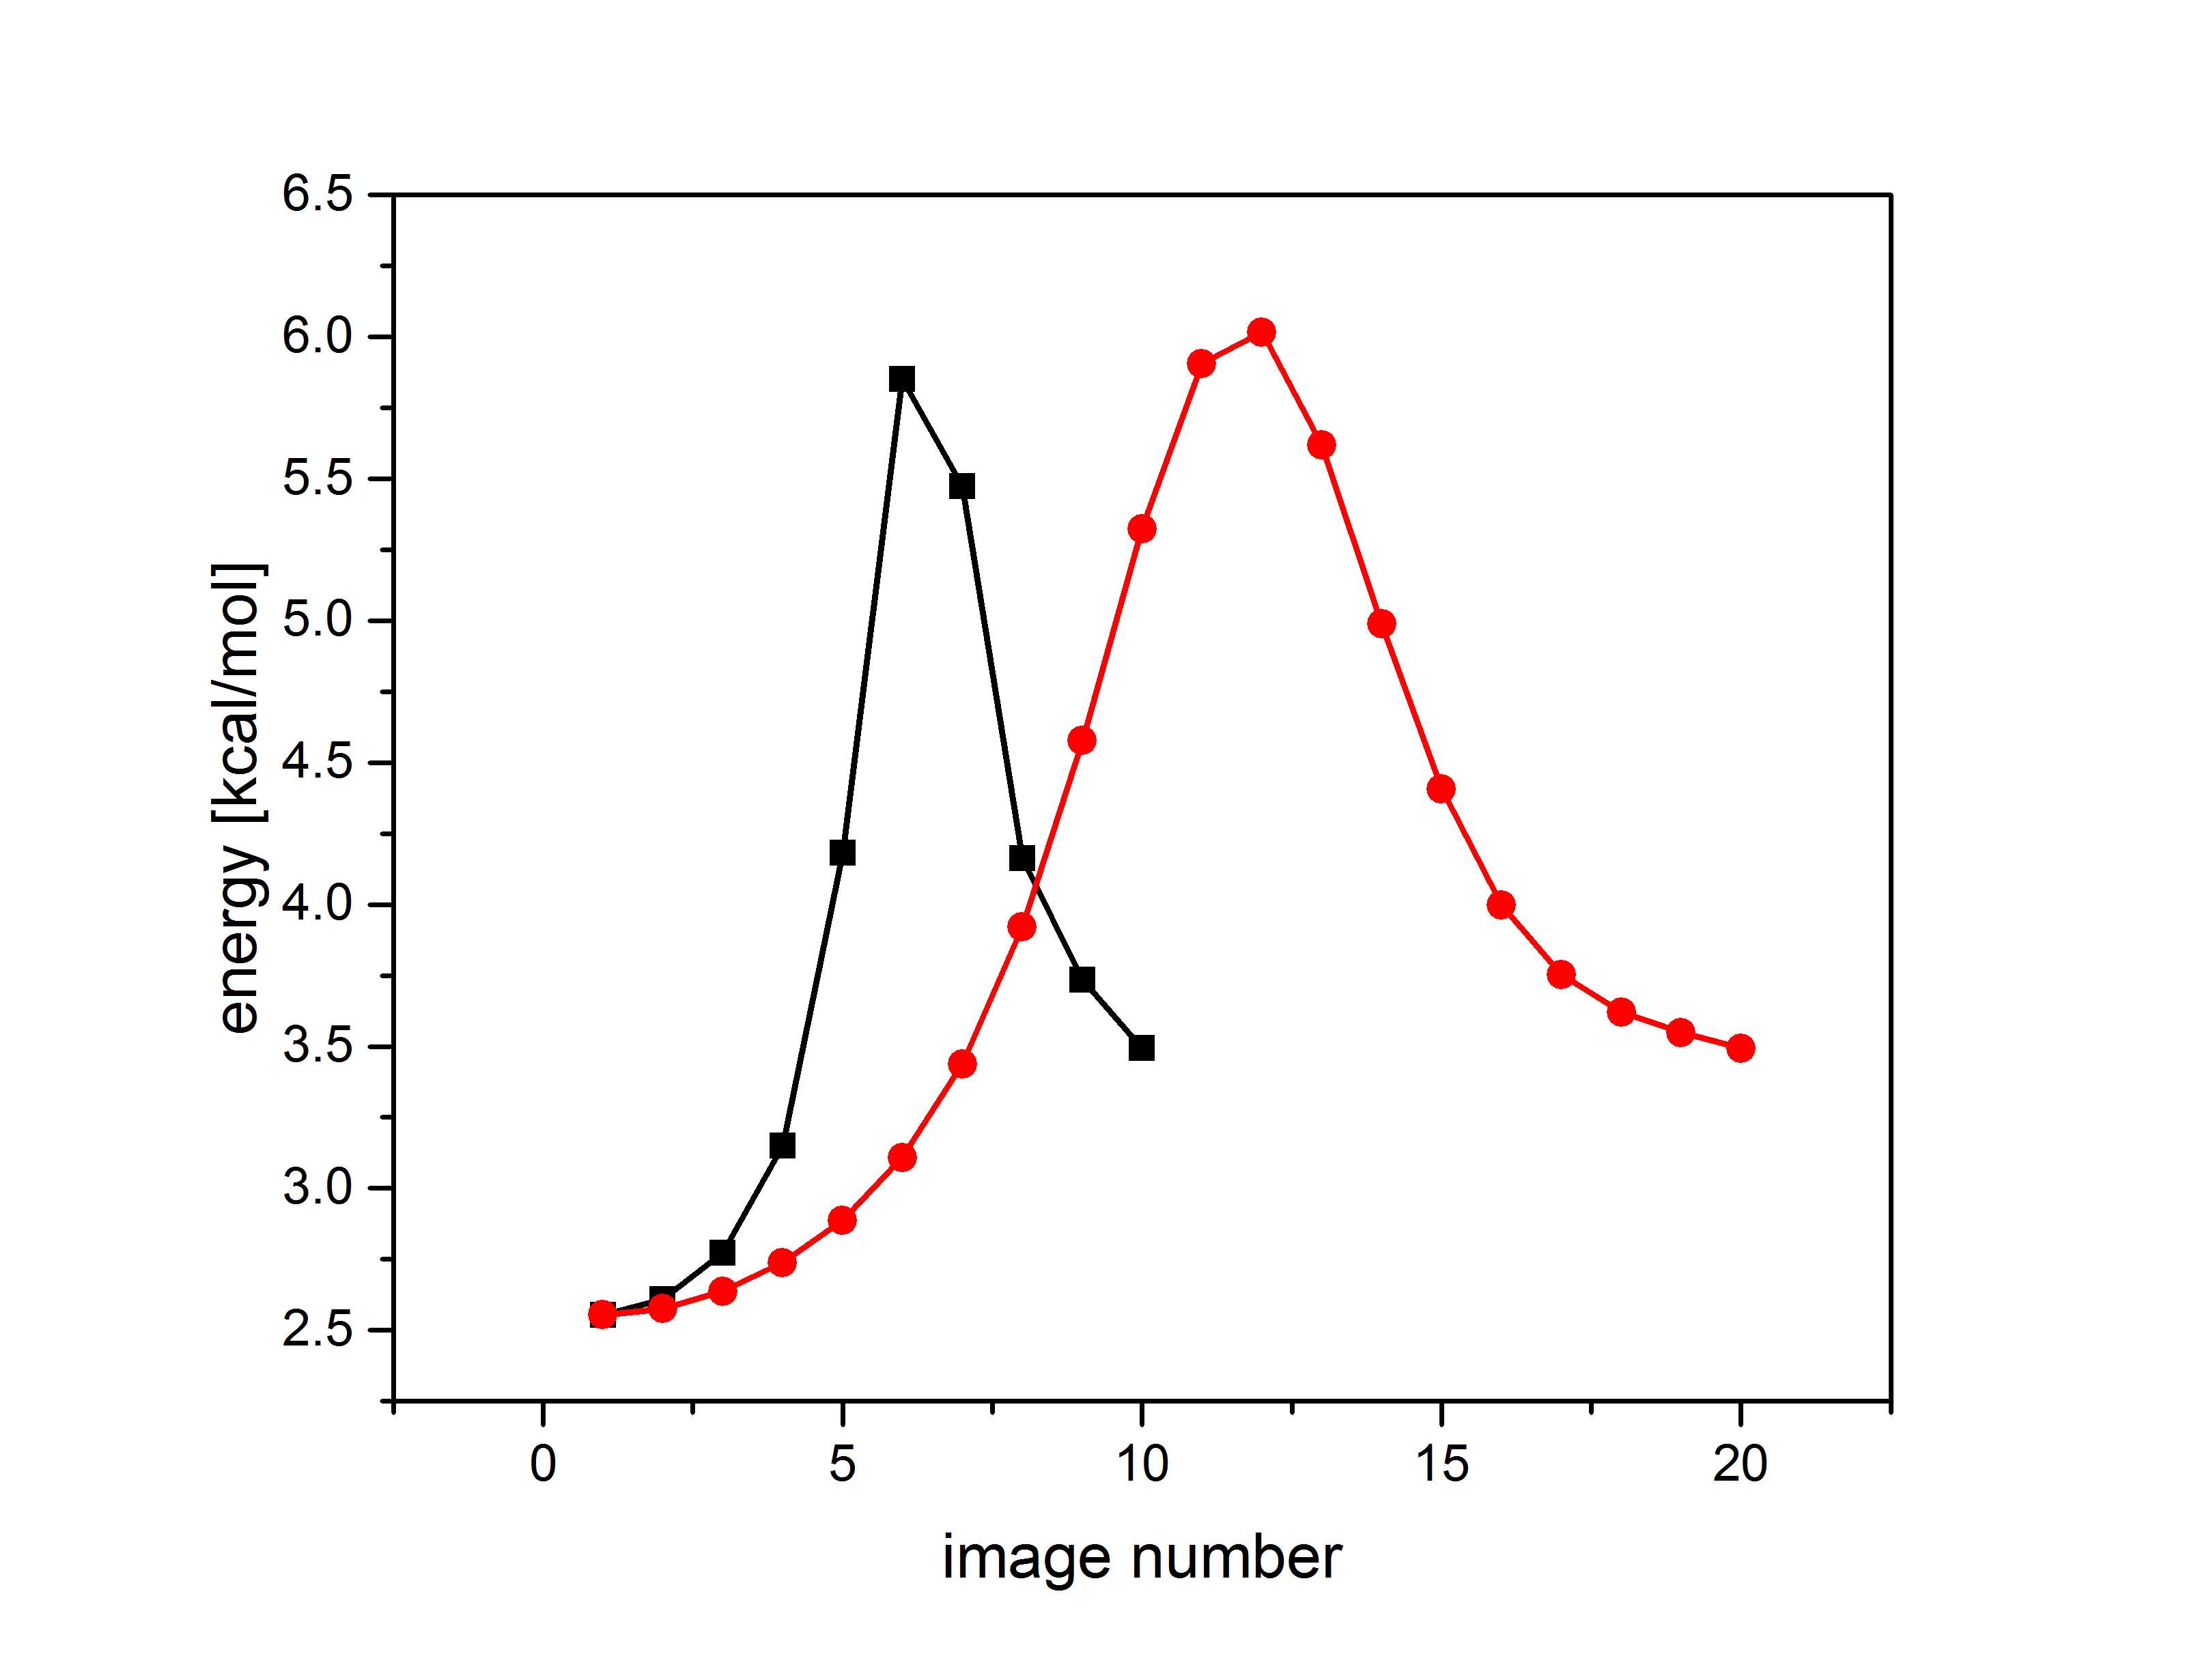
\includegraphics[scale=0.4]{NEB/pentane_standard_10_20.png}\caption{NEB pathway from a optimization carried out for 10/20 structures using the standard tangent-estimate. The OPLS-AA force field parameters were used.}
\label{fig:}
\end{figure}

\begin{figure}[H]
		\center
		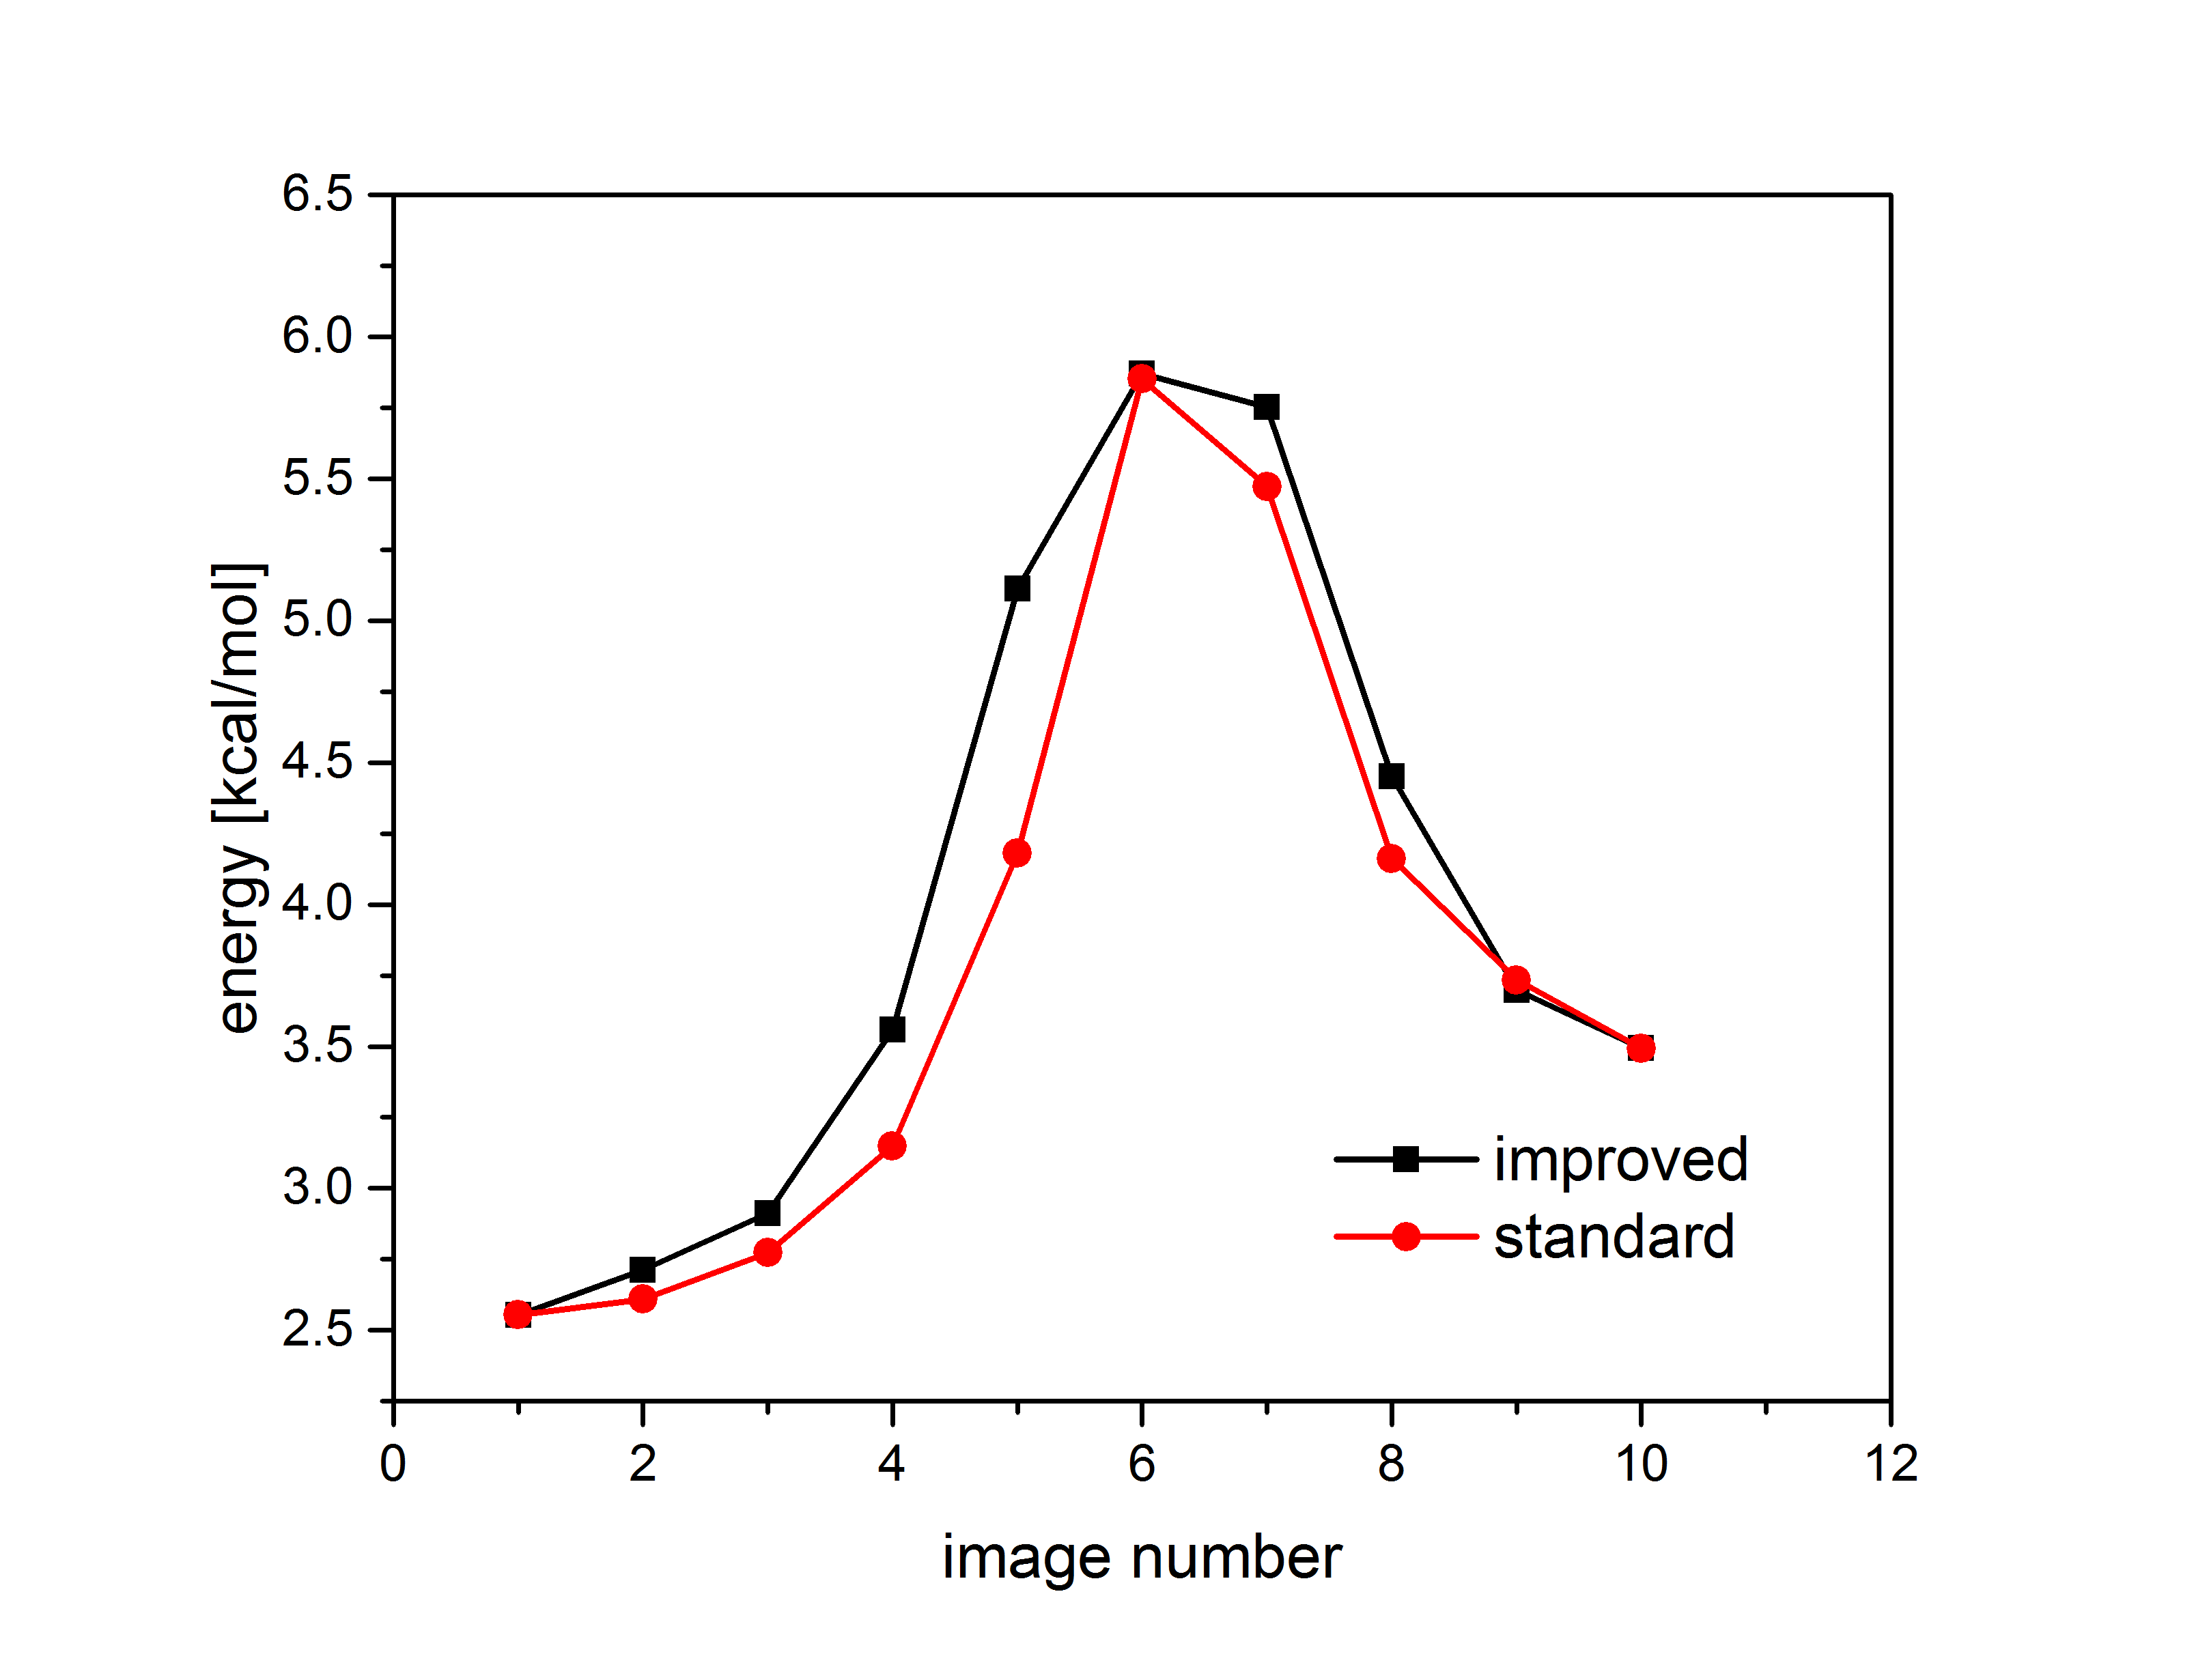
\includegraphics[scale=0.4]{NEB/pentane_standard_improved.png}\caption{Comparison between pathways obtained for a standard tangent estimate and an improved estimate calculation for the pentane transition.}
\label{fig:}
\end{figure}

\begin{figure}[H]
		\center
		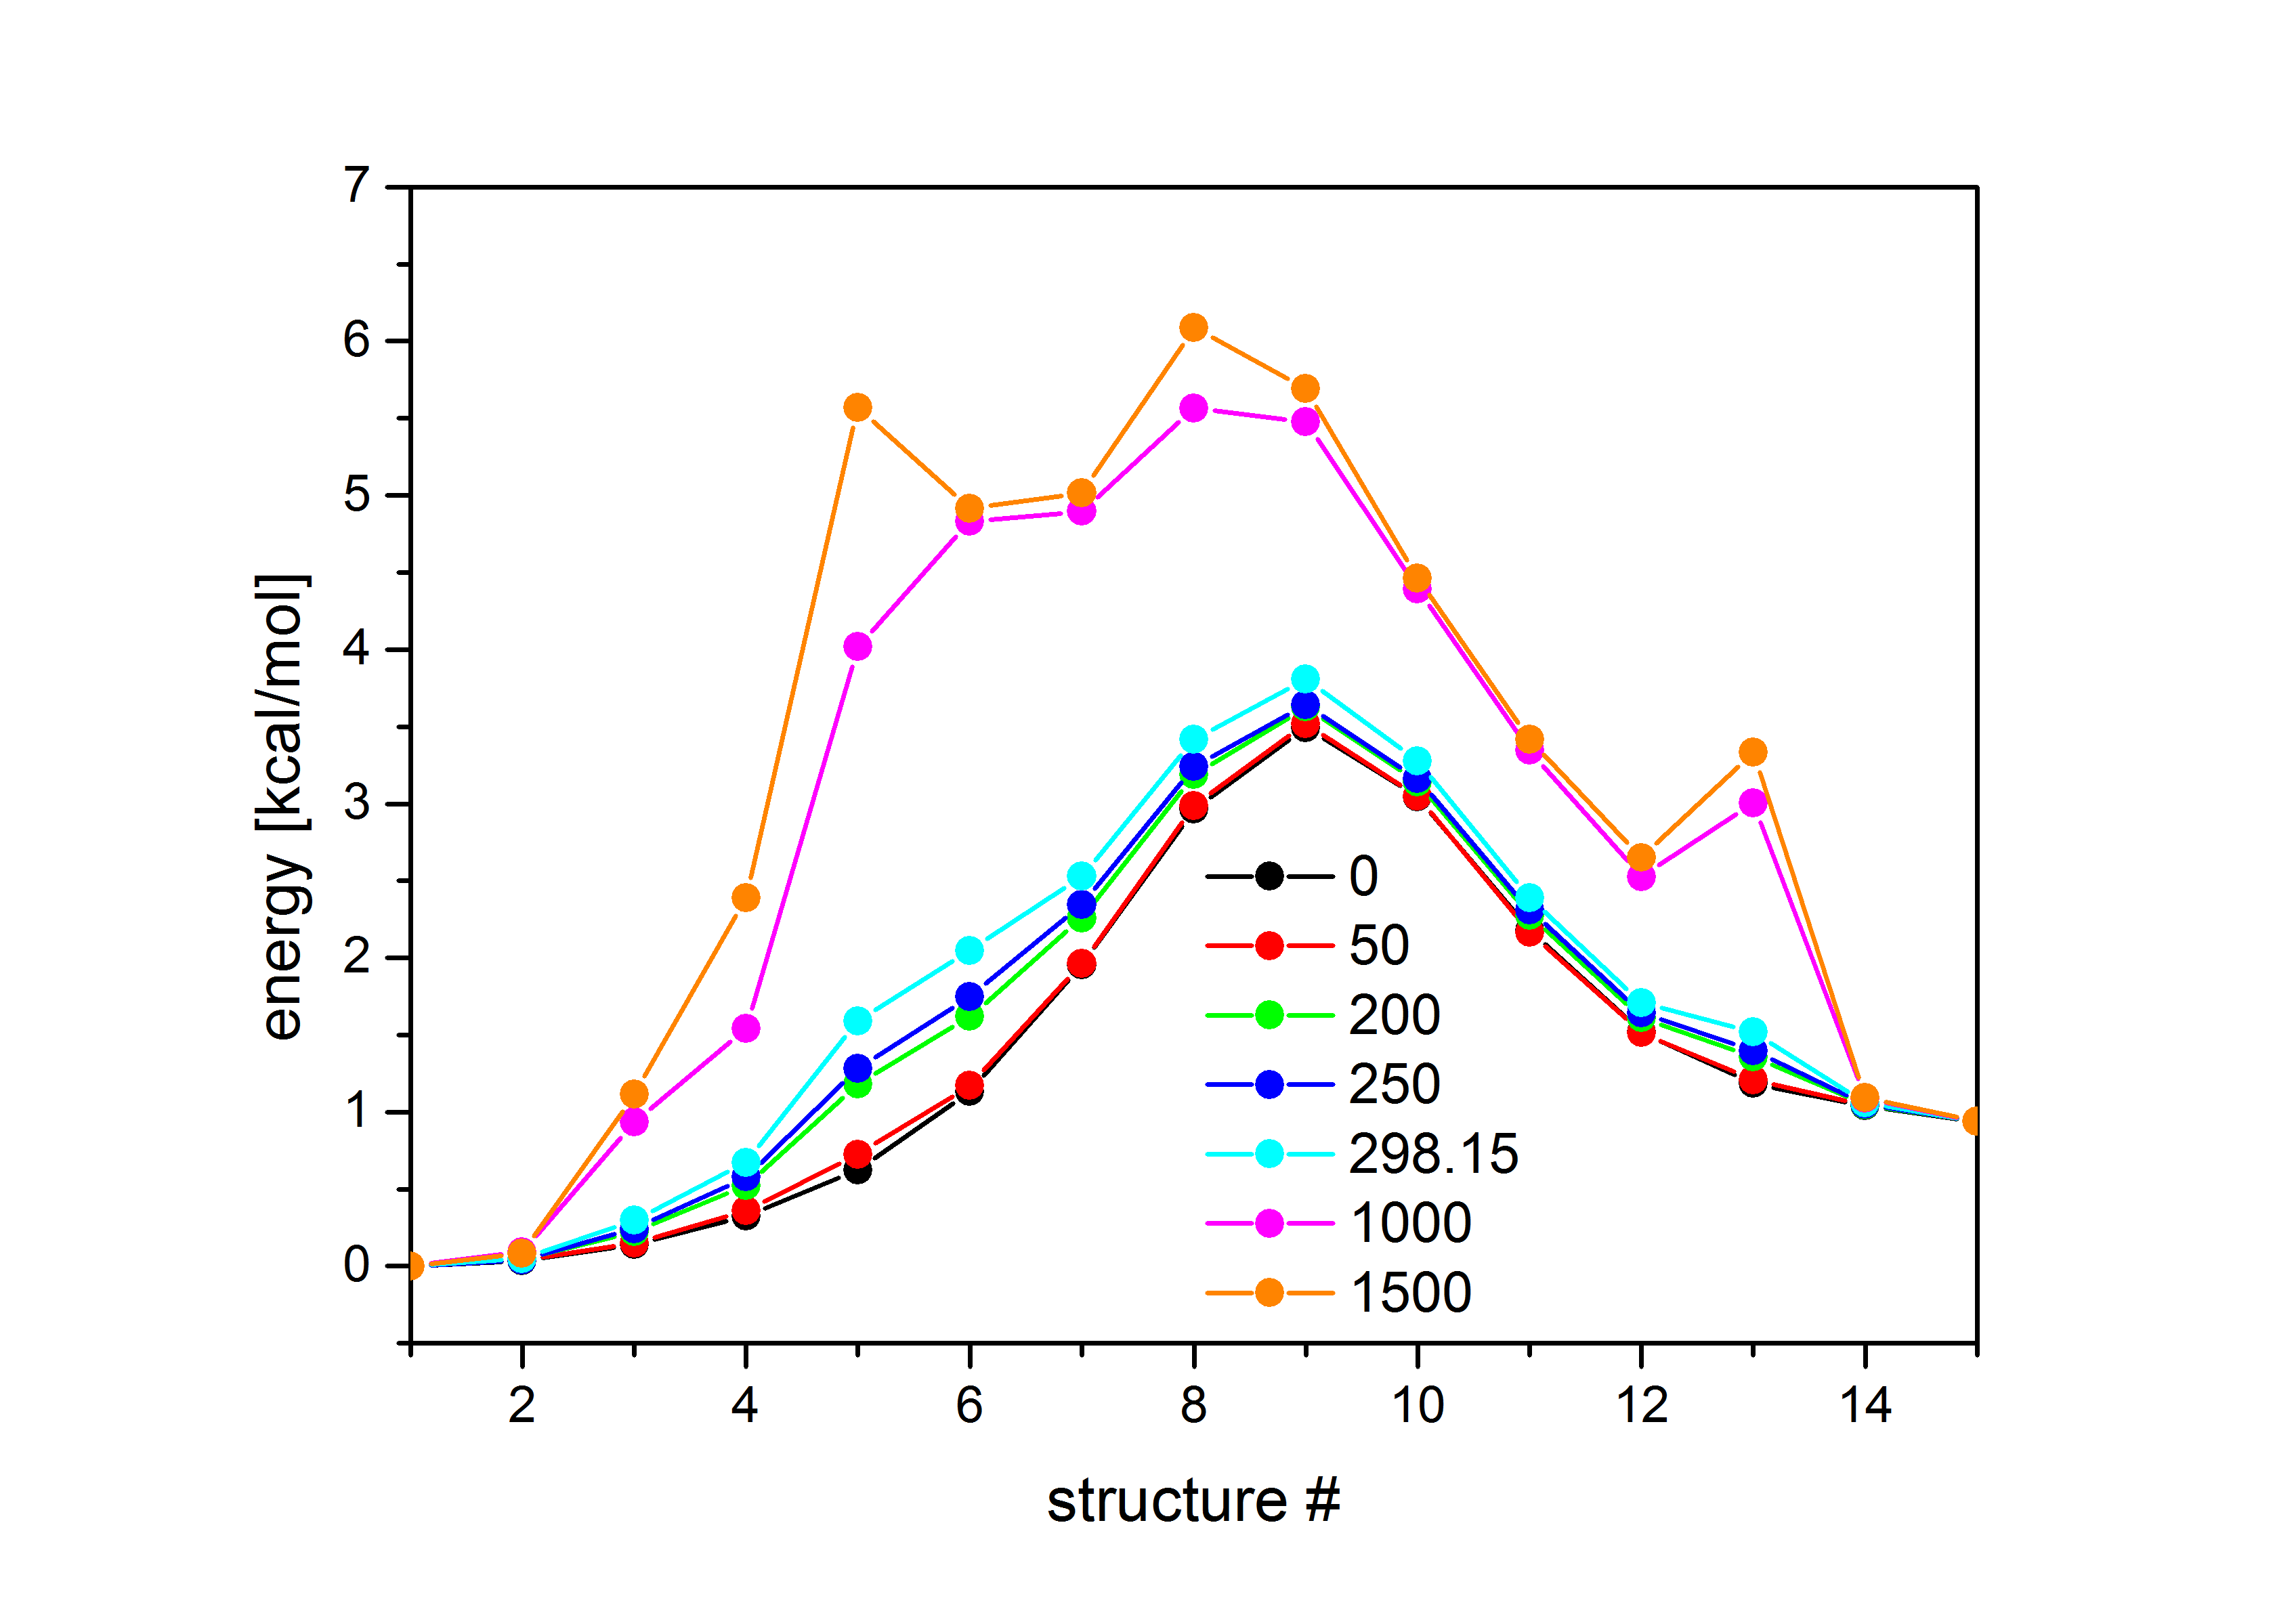
\includegraphics[scale=0.4]{NEB/neb_temp_pentane.png}\caption{The temperature dependent pathways for the pentane transition are shown.}
\label{fig:}
\end{figure}



\end{itemize}

\end{itemize}



\newpage

\paragraph{PATHOPT}\ac{pathopt}
\myCite{Grebner2013b,Weber2016} is a newly developed algorithm for finding reaction paths. It is a double-ended method that means, two structures are used. The main idea of the algorithm is, to make an initial guess between the start and final structure. This is performed by using the Nudged Elastic Band (NEB) approach. In a next step, this initial path is divided by perpendicular (n-1) dimensional hyperplanes. Subsequently, we perform global optimization on these hyperplanes. This is done with projected gradients (see figure \ref{fig:MCM}). The resulting minima are traces of possible reaction paths between the start and final structure. The number of planes can be varied and depends on the system, which is investigated. In addition, the connection method for the found traces of pathways can also be chosen. This pathways can be obtained in a direct manner via RMSD criterion or by using additional NEB simulations. The movement within the global optimization scheme can be chosen by using a distortion in Cartesian space or by applying a mixed move strategy (see figure \ref{fig:MIX}) and distorting dihedral angles as well.\newline

\begin{figure}[H]
		\center
		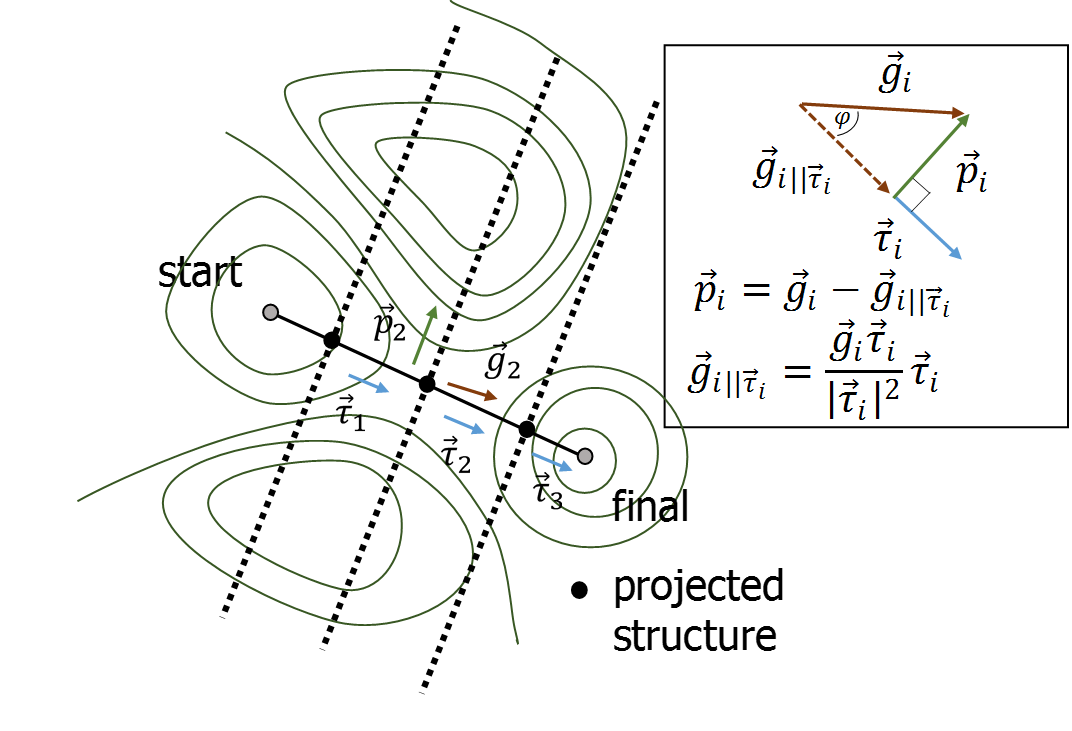
\includegraphics[scale=0.4]{Pathopt/MCM_scheme_new.png}\caption{Schematic representation of the Pathopt algorithm}
\label{fig:MCM}
\end{figure}

\begin{figure}[H]
		\center
		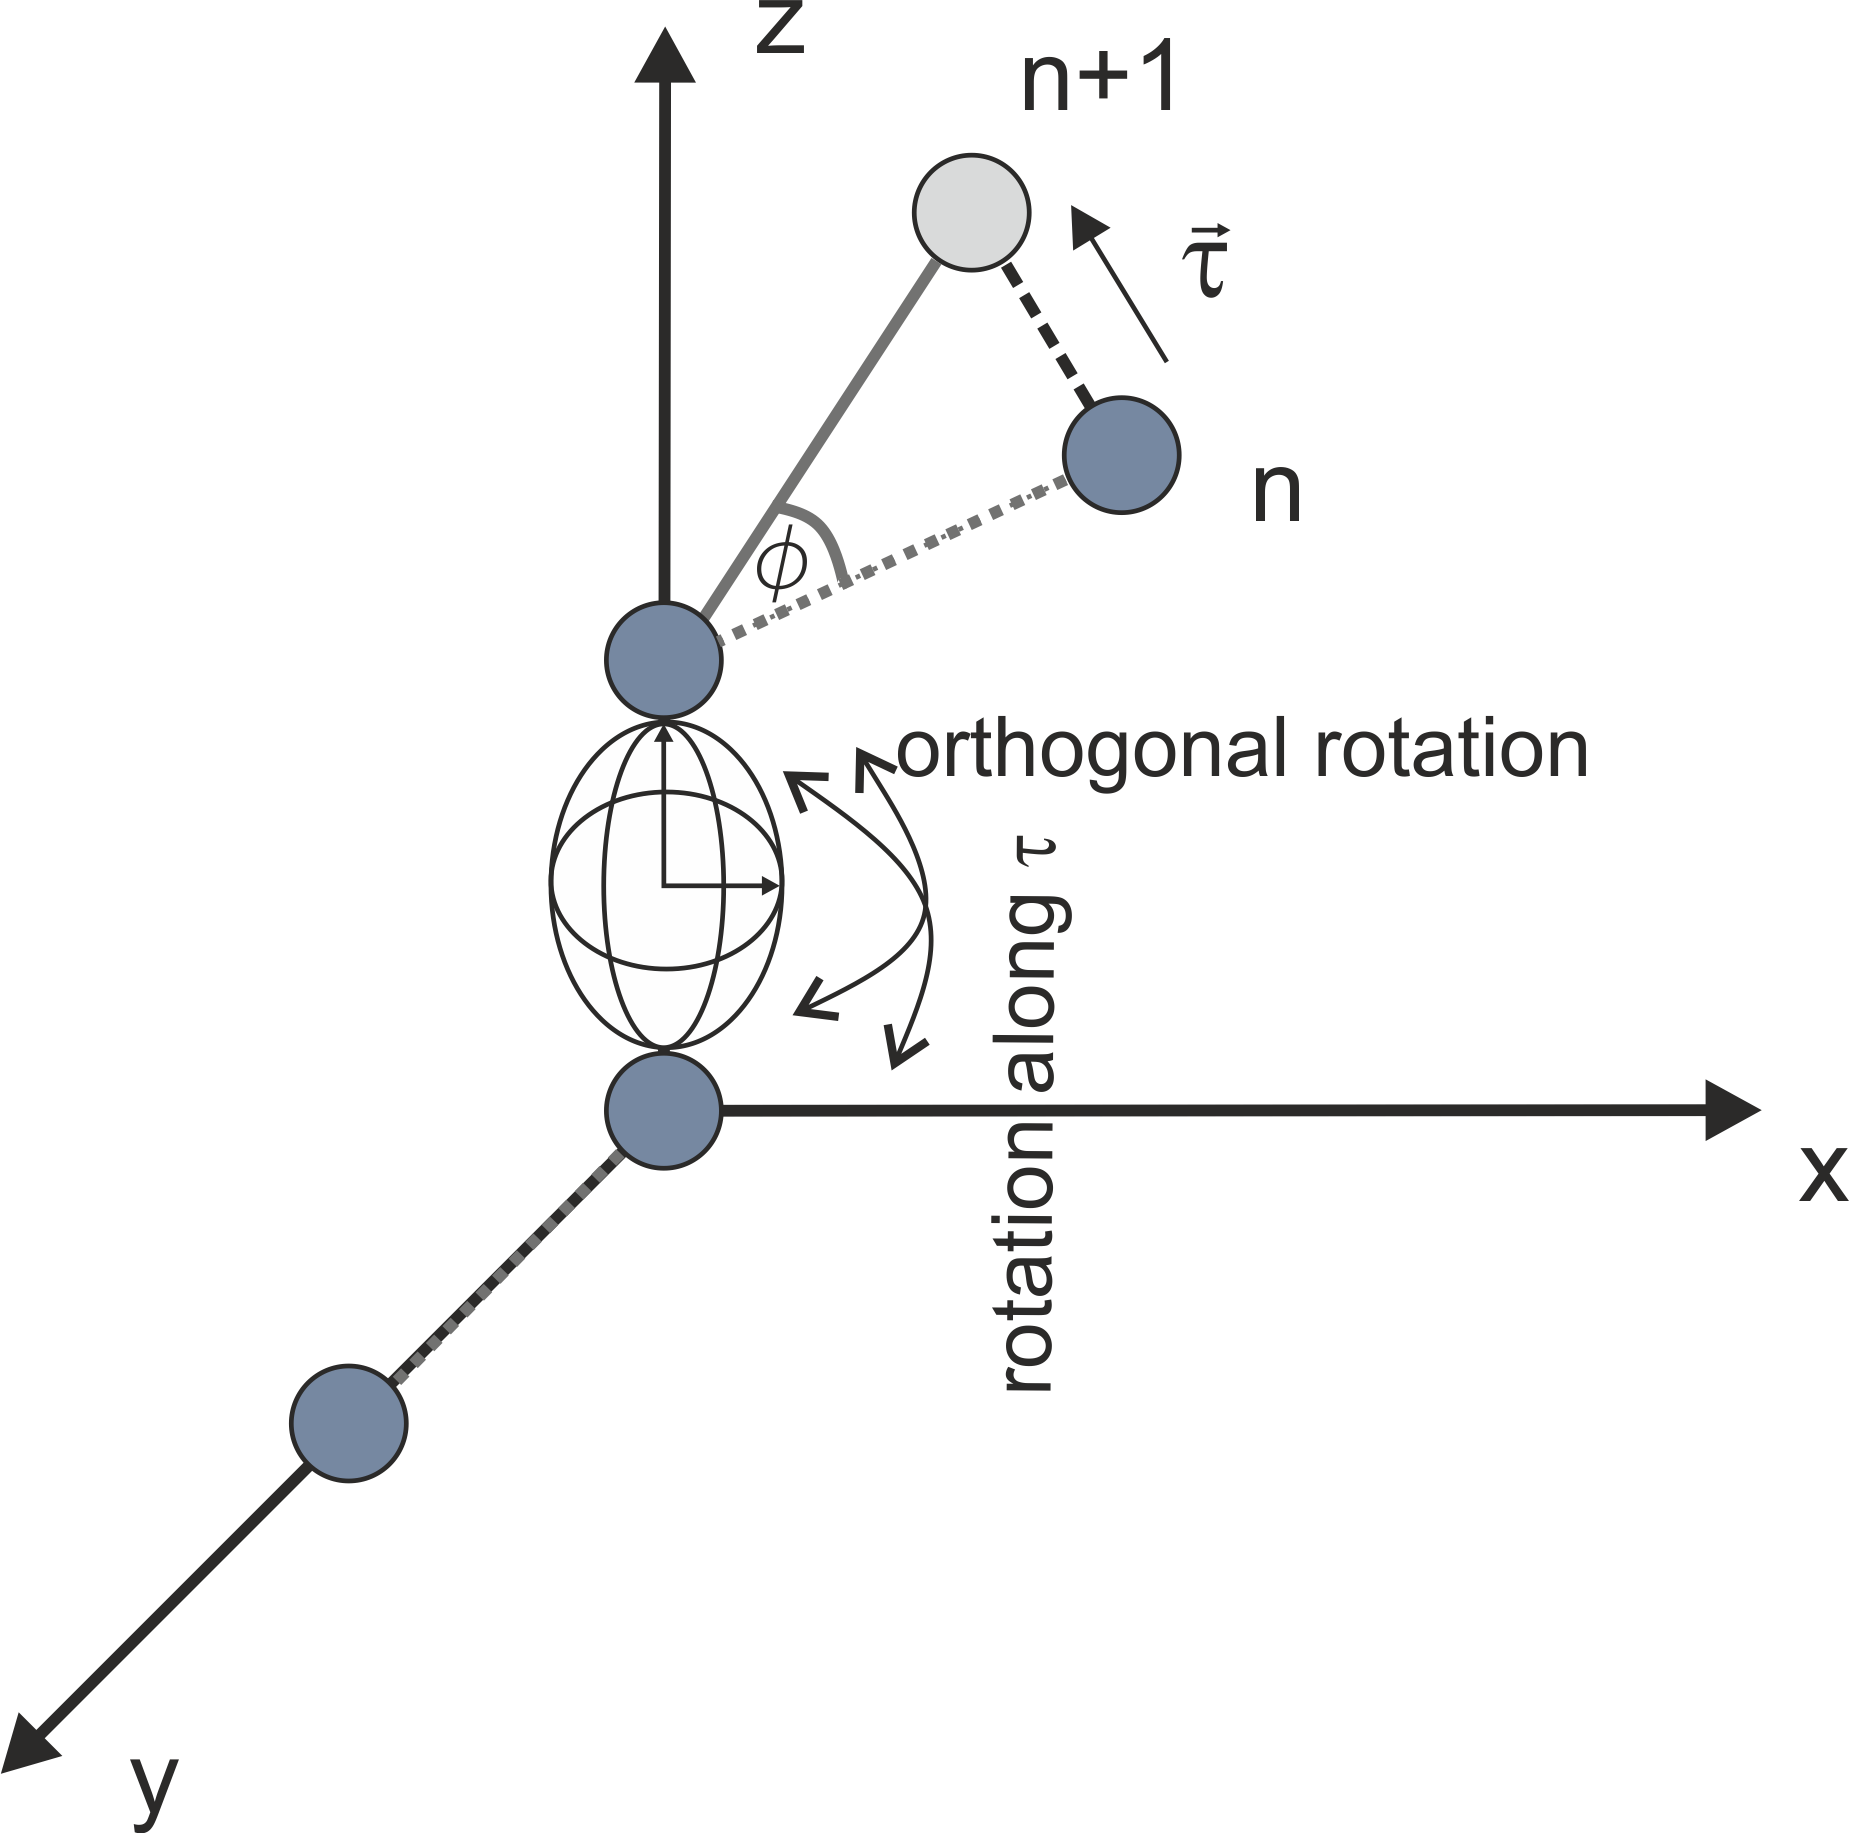
\includegraphics[scale=0.6]{Pathopt/grafik_rot_scheme.png}\caption{The mixed move strategy is illustrated by rotating only main dihedrals perpendicular to the connecting vectors $\tau$.}
\label{fig:MIX}
\end{figure}

PO calculations can be carried out by using various optional configurations. For the MCM procedure within PO the following settings can be varied: Steps, number of total MCM runs, Temperature criterion, stepsize, acceptance criteria, move-type and optimization settings (standard L-BFGS settings are used e.g. convergence).
\begin{itemize}

\item \texttt{NEB-PATHOPT-ITER} \textit{integer} - number of constraint MCM steps (see line \ref{appCAST:nebiter}).  

\item \texttt{NEB-PATHOPT-GLOBITER} \textit{integer} - number of total MC runs for multiple calculations (see line \ref{appCAST:nebglobiter}).

\item \texttt{NEB-PATHOPT-TEMP} \textit{floating point value} - assigns temperature value in K (see line \ref{appCAST:nebtemp}).

\item \texttt{NEB-PATHOPT-STEPSIZE} \textit{floating point value} - Cartesian step size in $\AA$ (see line \ref{appCAST:nebstepsize}).

\item \texttt{NEB-PATHOPT-MAXVAR} \textit{floating point value} - maximum allowed displacement in $\AA$ (see line \ref{appCAST:nebstepsize}).

\item \texttt{NEB-PATHOPT-ENERGY\_RANGE} \textit{floating point value} - maximum allowed energy difference with respect to starting structure  (see line \ref{appCAST:nebstepsize}).

\item \texttt{NEB-PATHOPT-MIXMOVE} \textit{bool} - de/-activates the dihedral movement approach (see line \ref{appCAST:nebmixmove}).

\item \texttt{NEB-PATHOPT-MODE} \textit{character string} - assigns the gradient calculation scheme: PROJECTED=projected gradients / BIAS=bias potential (needs a bias constant to be set (see line \ref{appCAST:nebmode}).

\item \texttt{NEB-PATHOPT-BIAS} \textit{floating point value} - bias constant in kcal/mol$\AA^{2}$ (see line \ref{appCAST:nebbiasconstant}).

\item \texttt{NEB-PATHOPT-MF\_PATHOPT} \textit{bool} - de/-activates the temperature dependent MAXFLUX optimization of PO pathways (uses standard temp. criterion) (see line \ref{appCAST:nebmfpathopt}).

\end{itemize}
\begin{itemize}

\item \textbf{Example calculation on Tridecaalanine and GlyAla-petide} \newline

\end{itemize}

In the following the standard parameters for the tridecaalanine calculation are given. The OPLS-AA method is used and for the PATHOPT procedure the standard gradient projection scheme is used. 

\begin{lstlisting}[
basicstyle=\footnotesize,
escapeinside={(@*}{*@)},
frame=single,
numbers=left,
]
name ala1.xyz

task NEB

interface OPLS-AA
paramfile             OPLS-AA_mod.prm

BFGSgrad              0.0001
BFGSmaxstep           1000


NEB-PATHOPT-FINAL ala2.arc
NEB-PATHOPT-IMAGES 22
NEB-PATHOPT-SPRING 1.0
NEB-PATHOPT-CLIMBING 1
NEB-PATHOPT-TAU 1
NEB-PATHOPT-TEMP 298.15
NEB-PATHOPT-ITER 1000
NEB-PATHOPT-GLOBITER 1
NEB-PATHOPT-MODE PROJECTED
NEB-PATHOPT-BIASCONSTANT 0.1
NEB-PATHOPT-MAXVAR 20.0
NEB-PATHOPT-ENERGY_RANGE 20.0
NEB-PATHOPT-STEPSIZE 1.4
NEB-PATHOPT-MIXMOVE 1 
NEB-PATHOPT-NEBCONN 0
NEB-PATHOPT-CONSTRAINT_GLOBAL 0


\end{lstlisting}

Input structure (ala1.arc): \newline

\begin{lstlisting}[
basicstyle=\footnotesize,
escapeinside={(@*}{*@)},
frame=single,
numbers=left,
]

  133
     1  N3    0.000000   -0.000000    0.000000   227     2     5     6     7
     2  CT    1.461000   -0.000000    0.000000   233     1     3     8     9
     3  C     1.963000    1.449000   -0.000000   174     2     4    13
     4  O     1.497000    2.242000   -0.816000   175     3
     5  H3   -0.415000    0.588000   -0.722000   230     1
     6  H3   -0.401000   -0.931000    0.019000   230     1
     7  H3   -0.282000    0.410000    0.903000   230     1
     8  HC    1.767000   -0.516000    0.907000    82     2
     9  CT    1.994000   -0.758000   -1.227000    77     2    10    11    12
    10  HC    1.661000   -1.797000   -1.225000    82     9
    11  HC    3.084000   -0.765000   -1.241000    82     9
    12  HC    1.658000   -0.300000   -2.158000    82     9
    13  N     2.910000    1.851000    0.852000   177     3    14    17
    14  CT    3.485000    1.181000    2.013000   163    13    15    18    19
    15  C     4.172000    2.273000    2.841000   174    14    16    23
    16  O     4.612000    3.278000    2.275000   175    15
    17  H     3.253000    2.800000    0.770000   180    13
    18  HC    2.700000    0.727000    2.619000    82    14
    19  CT    4.535000    0.148000    1.565000    77    14    20    21    22
    20  HC    4.097000   -0.681000    1.012000    82    19
    21  HC    5.049000   -0.279000    2.428000    82    19
    22  HC    5.298000    0.605000    0.933000    82    19
    23  N     4.282000    2.066000    4.154000   177    15    24    27
    24  CT    4.963000    2.945000    5.092000   163    23    25    28    29
    25  C     6.085000    2.158000    5.781000   174    24    26    33
    26  O     6.117000    0.926000    5.742000   175    25
    27  H     3.903000    1.214000    4.560000   180    23
    28  HC    5.403000    3.804000    4.581000    82    24
    29  CT    3.938000    3.434000    6.129000    77    24    30    31    32
    30  HC    3.130000    3.982000    5.644000    82    29
    31  HC    4.393000    4.102000    6.859000    82    29
    32  HC    3.489000    2.601000    6.672000    82    29
    33  N     6.998000    2.863000    6.459000   177    25    34    37
    34  CT    8.095000    2.282000    7.235000   163    33    35    38    39
    35  C     7.584000    1.800000    8.608000   174    34    36    43
    36  O     8.047000    2.254000    9.651000   175    35
    37  H     6.906000    3.866000    6.472000   180    33
    38  HC    8.496000    1.413000    6.708000    82    34
    39  CT    9.222000    3.323000    7.358000    77    34    40    41    42
    40  HC    9.592000    3.625000    6.378000    82    39
    41  HC   10.068000    2.915000    7.913000    82    39
    42  HC    8.888000    4.218000    7.886000    82    39
    43  N     6.606000    0.890000    8.585000   177    35    44    47
    44  CT    5.929000    0.304000    9.735000   163    43    45    48    49
    45  C     5.080000   -0.881000    9.268000   174    44    46    53
    46  O     5.202000   -1.981000    9.798000   175    45
    47  H     6.325000    0.563000    7.664000   180    43
    48  HC    6.683000   -0.073000   10.429000    82    44
    49  CT    5.051000    1.346000   10.456000    77    44    50    51    52
    50  HC    5.655000    2.145000   10.884000    82    49
    51  HC    4.501000    0.886000   11.278000    82    49
    52  HC    4.324000    1.801000    9.783000    82    49
    53  N     4.211000   -0.652000    8.276000   177    45    54    57
    54  CT    3.287000   -1.630000    7.717000   163    53    55    58    59
    55  C     2.906000   -1.201000    6.294000   174    54    56    63
    56  O     3.223000   -0.091000    5.861000   175    55
    57  H     4.192000    0.254000    7.828000   180    53
    58  HC    3.779000   -2.604000    7.661000    82    54
    59  CT    2.035000   -1.720000    8.610000    77    54    60    61    62
    60  HC    2.297000   -2.028000    9.623000    82    59
    61  HC    1.323000   -2.452000    8.227000    82    59
    62  HC    1.521000   -0.761000    8.676000    82    59
    63  N     2.211000   -2.084000    5.574000   177    55    64    67
    64  CT    1.689000   -1.857000    4.237000   163    63    65    68    69
    65  C     0.317000   -2.528000    4.147000   174    64    66    73
    66  O     0.128000   -3.615000    4.694000   175    65
    67  H     1.941000   -2.966000    5.989000   180    63
    68  HC    1.582000   -0.788000    4.046000    82    64
    69  CT    2.653000   -2.493000    3.223000    77    64    70    71    72
    70  HC    3.644000   -2.045000    3.290000    82    69
    71  HC    2.293000   -2.366000    2.203000    82    69
    72  HC    2.764000   -3.565000    3.397000    82    69
    73  N    -0.615000   -1.886000    3.445000   177    65    74    77
    74  CT   -1.936000   -2.384000    3.087000   163    73    75    78    79
    75  C    -2.108000   -2.295000    1.558000   174    74    76    83
    76  O    -1.127000   -2.322000    0.807000   175    75
    77  H    -0.370000   -0.953000    3.084000   180    73
    78  HC   -2.006000   -3.443000    3.341000    82    74
    79  CT   -3.016000   -1.624000    3.882000    77    74    80    81    82
    80  HC   -2.798000   -1.650000    4.950000    82    79
    81  HC   -4.001000   -2.070000    3.749000    82    79
    82  HC   -3.079000   -0.578000    3.586000    82    79
    83  N    -3.354000   -2.202000    1.081000   177    75    84    87
    84  CT   -3.728000   -2.293000   -0.330000   163    83    85    88    89
    85  C    -4.103000   -0.934000   -0.952000   174    84    86    93
    86  O    -4.781000   -0.917000   -1.976000   175    85
    87  H    -4.099000   -2.073000    1.747000   180    83
    88  HC   -2.900000   -2.689000   -0.921000    82    84
    89  CT   -4.897000   -3.290000   -0.433000    77    84    90    91    92
    90  HC   -4.628000   -4.260000   -0.014000    82    89
    91  HC   -5.180000   -3.458000   -1.473000    82    89
    92  HC   -5.782000   -2.928000    0.090000    82    89
    93  N    -3.674000    0.195000   -0.371000   177    85    94    97
    94  CT   -3.900000    1.538000   -0.902000   163    93    95    98    99
    95  C    -2.551000    2.162000   -1.304000   174    94    96   103
    96  O    -1.583000    1.450000   -1.587000   175    95
    97  H    -3.105000    0.165000    0.477000   180    93
    98  HC   -4.505000    1.502000   -1.810000    82    94
    99  CT   -4.666000    2.368000    0.145000    77    94   100   101   102
   100  HC   -5.575000    1.855000    0.459000    82    99
   101  HC   -4.968000    3.339000   -0.247000    82    99
   102  HC   -4.059000    2.539000    1.033000    82    99
   103  N    -2.481000    3.496000   -1.323000   177    95   104   107
   104  CT   -1.267000    4.283000   -1.487000   163   103   105   108   109
   105  C    -0.922000    4.822000   -0.095000   174   104   106   113
   106  O    -1.811000    5.315000    0.600000   175   105
   107  H    -3.304000    4.011000   -1.053000   180   103
   108  HC   -0.448000    3.676000   -1.874000    82   104
   109  CT   -1.547000    5.435000   -2.463000    77   104   110   111   112
   110  HC   -1.842000    5.057000   -3.442000    82   109
   111  HC   -0.657000    6.050000   -2.603000    82   109
   112  HC   -2.343000    6.089000   -2.102000    82   109
   113  N     0.344000    4.698000    0.321000   177   105   114   117
   114  CT    0.915000    5.067000    1.626000   163   113   115   118   119
   115  C     0.554000    4.059000    2.729000   174   114   116   123
   116  O     1.417000    3.679000    3.515000   175   115
   117  H     0.964000    4.194000   -0.302000   180   113
   118  HC    1.995000    4.986000    1.496000    82   114
   119  CT    0.625000    6.522000    2.038000    77   114   120   121   122
   120  HC    0.916000    7.222000    1.255000    82   119
   121  HC    1.185000    6.783000    2.937000    82   119
   122  HC   -0.430000    6.685000    2.262000    82   119
   123  N    -0.705000    3.613000    2.763000   177   115   124   127
   124  CT   -1.175000    2.467000    3.524000   222   123   125   128   129
   125  C    -1.049000    1.269000    2.583000   210   124   126   133
   126  O2   -0.000000    0.593000    2.580000   211   125
   127  H    -1.352000    4.033000    2.107000   180   123
   128  HC   -0.545000    2.292000    4.399000    82   124
   129  CT   -2.622000    2.709000    3.981000    77   124   130   131   132
   130  HC   -2.679000    3.559000    4.661000    82   129
   131  HC   -3.011000    1.838000    4.508000    82   129
   132  HC   -3.284000    2.909000    3.140000    82   129
   133  O2   -1.948000    0.995000    1.762000   211   125

\end{lstlisting}

Input structure 2 (ala2.arc): \newline

\begin{lstlisting}[
basicstyle=\footnotesize,
escapeinside={(@*}{*@)},
frame=single,
numbers=left,
]

  133
     1  N3     0.364558    0.471283    0.336934   227     2     5     6     7
     2  CT     1.122582    1.089650   -0.746370   233     1     3     8     9
     3  C      1.146753    2.607327   -0.523589   174     2     4    13
     4  O      0.195284    3.286015   -0.892547   175     3
     5  H3    -0.551878    0.916236    0.436559   230     1
     6  H3     0.248087   -0.532694    0.230849   230     1
     7  H3     0.844314    0.603110    1.244630   230     1
     8  HC     2.135483    0.693100   -0.722507    82     2
     9  CT     0.517872    0.722197   -2.111722    77     2    10    11    12
    10  HC    -0.523885    1.039957   -2.186698    82     9
    11  HC     0.549508   -0.354270   -2.282869    82     9
    12  HC     1.065509    1.201189   -2.924284    82     9
    13  N      2.178818    3.198847    0.078918   177     3    14    17
    14  CT     3.360642    2.626253    0.713958   163    13    15    18    19
    15  C      3.624637    3.422485    1.998460   174    14    16    23
    16  O      3.042835    4.493614    2.194802   175    15
    17  H      2.107424    4.198450    0.213656   180    13
    18  HC     3.211407    1.586949    0.987211    82    14
    19  CT     4.553856    2.731182   -0.251321    77    14    20    21    22
    20  HC     4.366982    2.190381   -1.179116    82    19
    21  HC     5.456575    2.309133    0.195797    82    19
    22  HC     4.775412    3.769312   -0.505135    82    19
    23  N      4.519136    2.906682    2.840358   177    15    24    27
    24  CT     5.087370    3.567480    4.004334   163    23    25    28    29
    25  C      6.494805    4.049839    3.625106   174    24    26    33
    26  O      7.030457    3.698424    2.571618   175    25
    27  H      4.973399    2.030264    2.593019   180    23
    28  HC     4.471251    4.415991    4.308886    82    24
    29  CT     5.187810    2.545480    5.151654    77    24    30    31    32
    30  HC     4.236290    2.046753    5.323468    82    29
    31  HC     5.466822    3.031885    6.085630    82    29
    32  HC     5.924932    1.769640    4.949651    82    29
    33  N      7.138436    4.823954    4.502583   177    25    34    37
    34  CT     8.502830    5.318054    4.311728   163    33    35    38    39
    35  C      9.538332    4.250856    4.729180   174    34    36    43
    36  O     10.441898    4.535352    5.510622   175    35
    37  H      6.668968    5.063956    5.361579   180    33
    38  HC     8.671517    5.542422    3.256022    82    34
    39  CT     8.652719    6.629782    5.102295    77    34    40    41    42
    40  HC     7.910101    7.364754    4.792393    82    39
    41  HC     9.635228    7.073381    4.937232    82    39
    42  HC     8.543637    6.469602    6.175397    82    39
    43  N      9.395425    3.023613    4.208162   177    35    44    47
    44  CT    10.244640    1.854708    4.443575   163    43    45    48    49
    45  C      9.709152    0.648583    3.662193   174    44    46    53
    46  O     10.418255    0.065462    2.847102   175    45
    47  H      8.647085    2.914834    3.529037   180    43
    48  HC    11.244686    2.077642    4.067388    82    44
    49  CT    10.343337    1.494004    5.943323    77    44    50    51    52
    50  HC    10.896908    2.246758    6.503313    82    49
    51  HC    10.874704    0.551449    6.083693    82    49
    52  HC     9.361106    1.392308    6.404749    82    49
    53  N      8.456738    0.267755    3.938931   177    45    54    57
    54  CT     7.780402   -0.917558    3.412811   163    53    55    58    59
    55  C      6.480516   -0.509419    2.704498   174    54    56    63
    56  O      6.164809    0.674931    2.602772   175    55
    57  H      7.914744    0.864838    4.541159   180    53
    58  HC     8.408601   -1.426403    2.678910    82    54
    59  CT     7.497036   -1.874031    4.587200    77    54    60    61    62
    60  HC     8.417115   -2.125172    5.116006    82    59
    61  HC     7.059615   -2.813506    4.246516    82    59
    62  HC     6.809230   -1.431906    5.309753    82    59
    63  N      5.705359   -1.481334    2.218842   177    55    64    67
    64  CT     4.410346   -1.260682    1.593704   163    63    65    68    69
    65  C      3.494957   -2.433629    1.943255   174    64    66    73
    66  O      3.929572   -3.584104    1.895072   175    65
    67  H      5.971179   -2.450641    2.333016   180    63
    68  HC     3.964351   -0.342119    1.975834    82    64
    69  CT     4.599259   -1.159192    0.070395    77    64    70    71    72
    70  HC     5.204584   -0.291195   -0.192066    82    69
    71  HC     3.641606   -1.066086   -0.440318    82    69
    72  HC     5.095883   -2.044413   -0.330540    82    69
    73  N      2.239053   -2.131947    2.276170   177    65    74    77
    74  CT     1.147929   -3.077935    2.478659   163    73    75    78    79
    75  C     -0.019828   -2.701127    1.547386   174    74    76    83
    76  O      0.204484   -2.197456    0.441798   175    75
    77  H      2.000773   -1.138366    2.369876   180    73
    78  HC     1.468071   -4.074025    2.166706    82    74
    79  CT     0.771341   -3.146007    3.971787    77    74    80    81    82
    80  HC     1.649657   -3.348590    4.584754    82    79
    81  HC     0.057678   -3.946006    4.168827    82    79
    82  HC     0.332423   -2.213599    4.323866    82    79
    83  N     -1.263229   -2.950015    1.971071   177    75    84    87
    84  CT    -2.473146   -2.867312    1.152417   163    83    85    88    89
    85  C     -3.304358   -1.588192    1.371095   174    84    86    93
    86  O     -4.413471   -1.511518    0.848514   175    85
    87  H     -1.374335   -3.241278    2.929597   180    83
    88  HC    -2.209490   -2.886553    0.092862    82    84
    89  CT    -3.320446   -4.118431    1.447917    77    84    90    91    92
    90  HC    -2.760216   -5.031725    1.245898    82    89
    91  HC    -4.214431   -4.145521    0.822299    82    89
    92  HC    -3.649694   -4.145640    2.487668    82    89
    93  N     -2.807654   -0.592545    2.115630   177    85    94    97
    94  CT    -3.489448    0.673989    2.378454   163    93    95    98    99
    95  C     -2.716813    1.817295    1.697869   174    94    96   103
    96  O     -1.977067    1.598757    0.736396   175    95
    97  H     -1.861679   -0.651159    2.503034   180    93
    98  HC    -4.496007    0.675019    1.955690    82    94
    99  CT    -3.606547    0.866181    3.904455    77    94   100   101   102
   100  HC    -4.076518    0.000539    4.371517    82    99
   101  HC    -4.213848    1.735413    4.159394    82    99
   102  HC    -2.625540    1.000019    4.363578    82    99
   103  N     -2.872020    3.037369    2.212580   177    95   104   107
   104  CT    -2.040404    4.204959    1.961449   163   103   105   108   109
   105  C     -1.420102    4.527654    3.326096   174   104   106   113
   106  O     -2.109778    4.406381    4.337814   175   105
   107  H     -3.503535    3.138145    2.995083   180   103
   108  HC    -1.257001    3.990102    1.233080    82   104
   109  CT    -2.927789    5.352463    1.461079    77   104   110   111   112
   110  HC    -3.422729    5.081486    0.527936    82   109
   111  HC    -2.337436    6.248877    1.270187    82   109
   112  HC    -3.699764    5.611467    2.186989    82   109
   113  N     -0.127719    4.879004    3.360365   177   105   114   117
   114  CT     0.736446    5.025222    4.545331   163   113   115   118   119
   115  C      1.286007    3.676335    5.043901   174   114   116   123
   116  O      2.289860    3.652879    5.751564   175   115
   117  H      0.353827    4.976612    2.478811   180   113
   118  HC     1.606845    5.579677    4.192718    82   114
   119  CT     0.116651    5.853197    5.688308    77   114   120   121   122
   120  HC    -0.309309    6.786982    5.322712    82   119
   121  HC     0.877475    6.103701    6.428798    82   119
   122  HC    -0.664217    5.303137    6.214447    82   119
   123  N      0.637609    2.569695    4.667622   177   115   124   127
   124  CT     1.085960    1.196638    4.798430   222   123   125   128   129
   125  C      0.800266    0.557306    3.440574   210   124   126   133
   126  O2     1.682175    0.555939    2.556020   211   125
   127  H     -0.223874    2.692482    4.159419   180   123
   128  HC     2.160370    1.156144    4.976397    82   124
   129  CT     0.341473    0.507421    5.953095    77   124   130   131   132
   130  HC     0.536811    1.014794    6.897783    82   129
   131  HC     0.670773   -0.525842    6.060726    82   129
   132  HC    -0.736624    0.498476    5.793444    82   129
   133  O2    -0.322015    0.078066    3.186905   211   125


\end{lstlisting} 

After a successful PO calculation one should obtain the following files and folders: PATHOPT\_BASIN\_ENERGIES\_X.dat, PATHOPT\_STRUCTURES\_X\_Y.arc, arrhenius\_global.dat and folders 1-3. X and Y stand for the global run and concerning hyperplane.\newline

\begin{itemize}

\item \texttt{PATHOPT\_BASIN\_ENERGIES} - contains the energies of the accepted structures with mcstep number, hyperplane number and energy in kcal/mol.

\item \texttt{PATHOPT\_STRUCTURES} - contains the structures found on each hyperplane in TINKER format.

\item \texttt{FOLDERS 1-3} - the connected pathways sorted as energy and structure files, whereas folder 1 contains next minimum RMSD moves along the hyperplanes and further on by increasing order.


\item \texttt{arrhenius\_global.dat} - the arrhenius rates are given, but without any preexponential factor included.

\end{itemize}

\begin{figure}[H]
		\center
		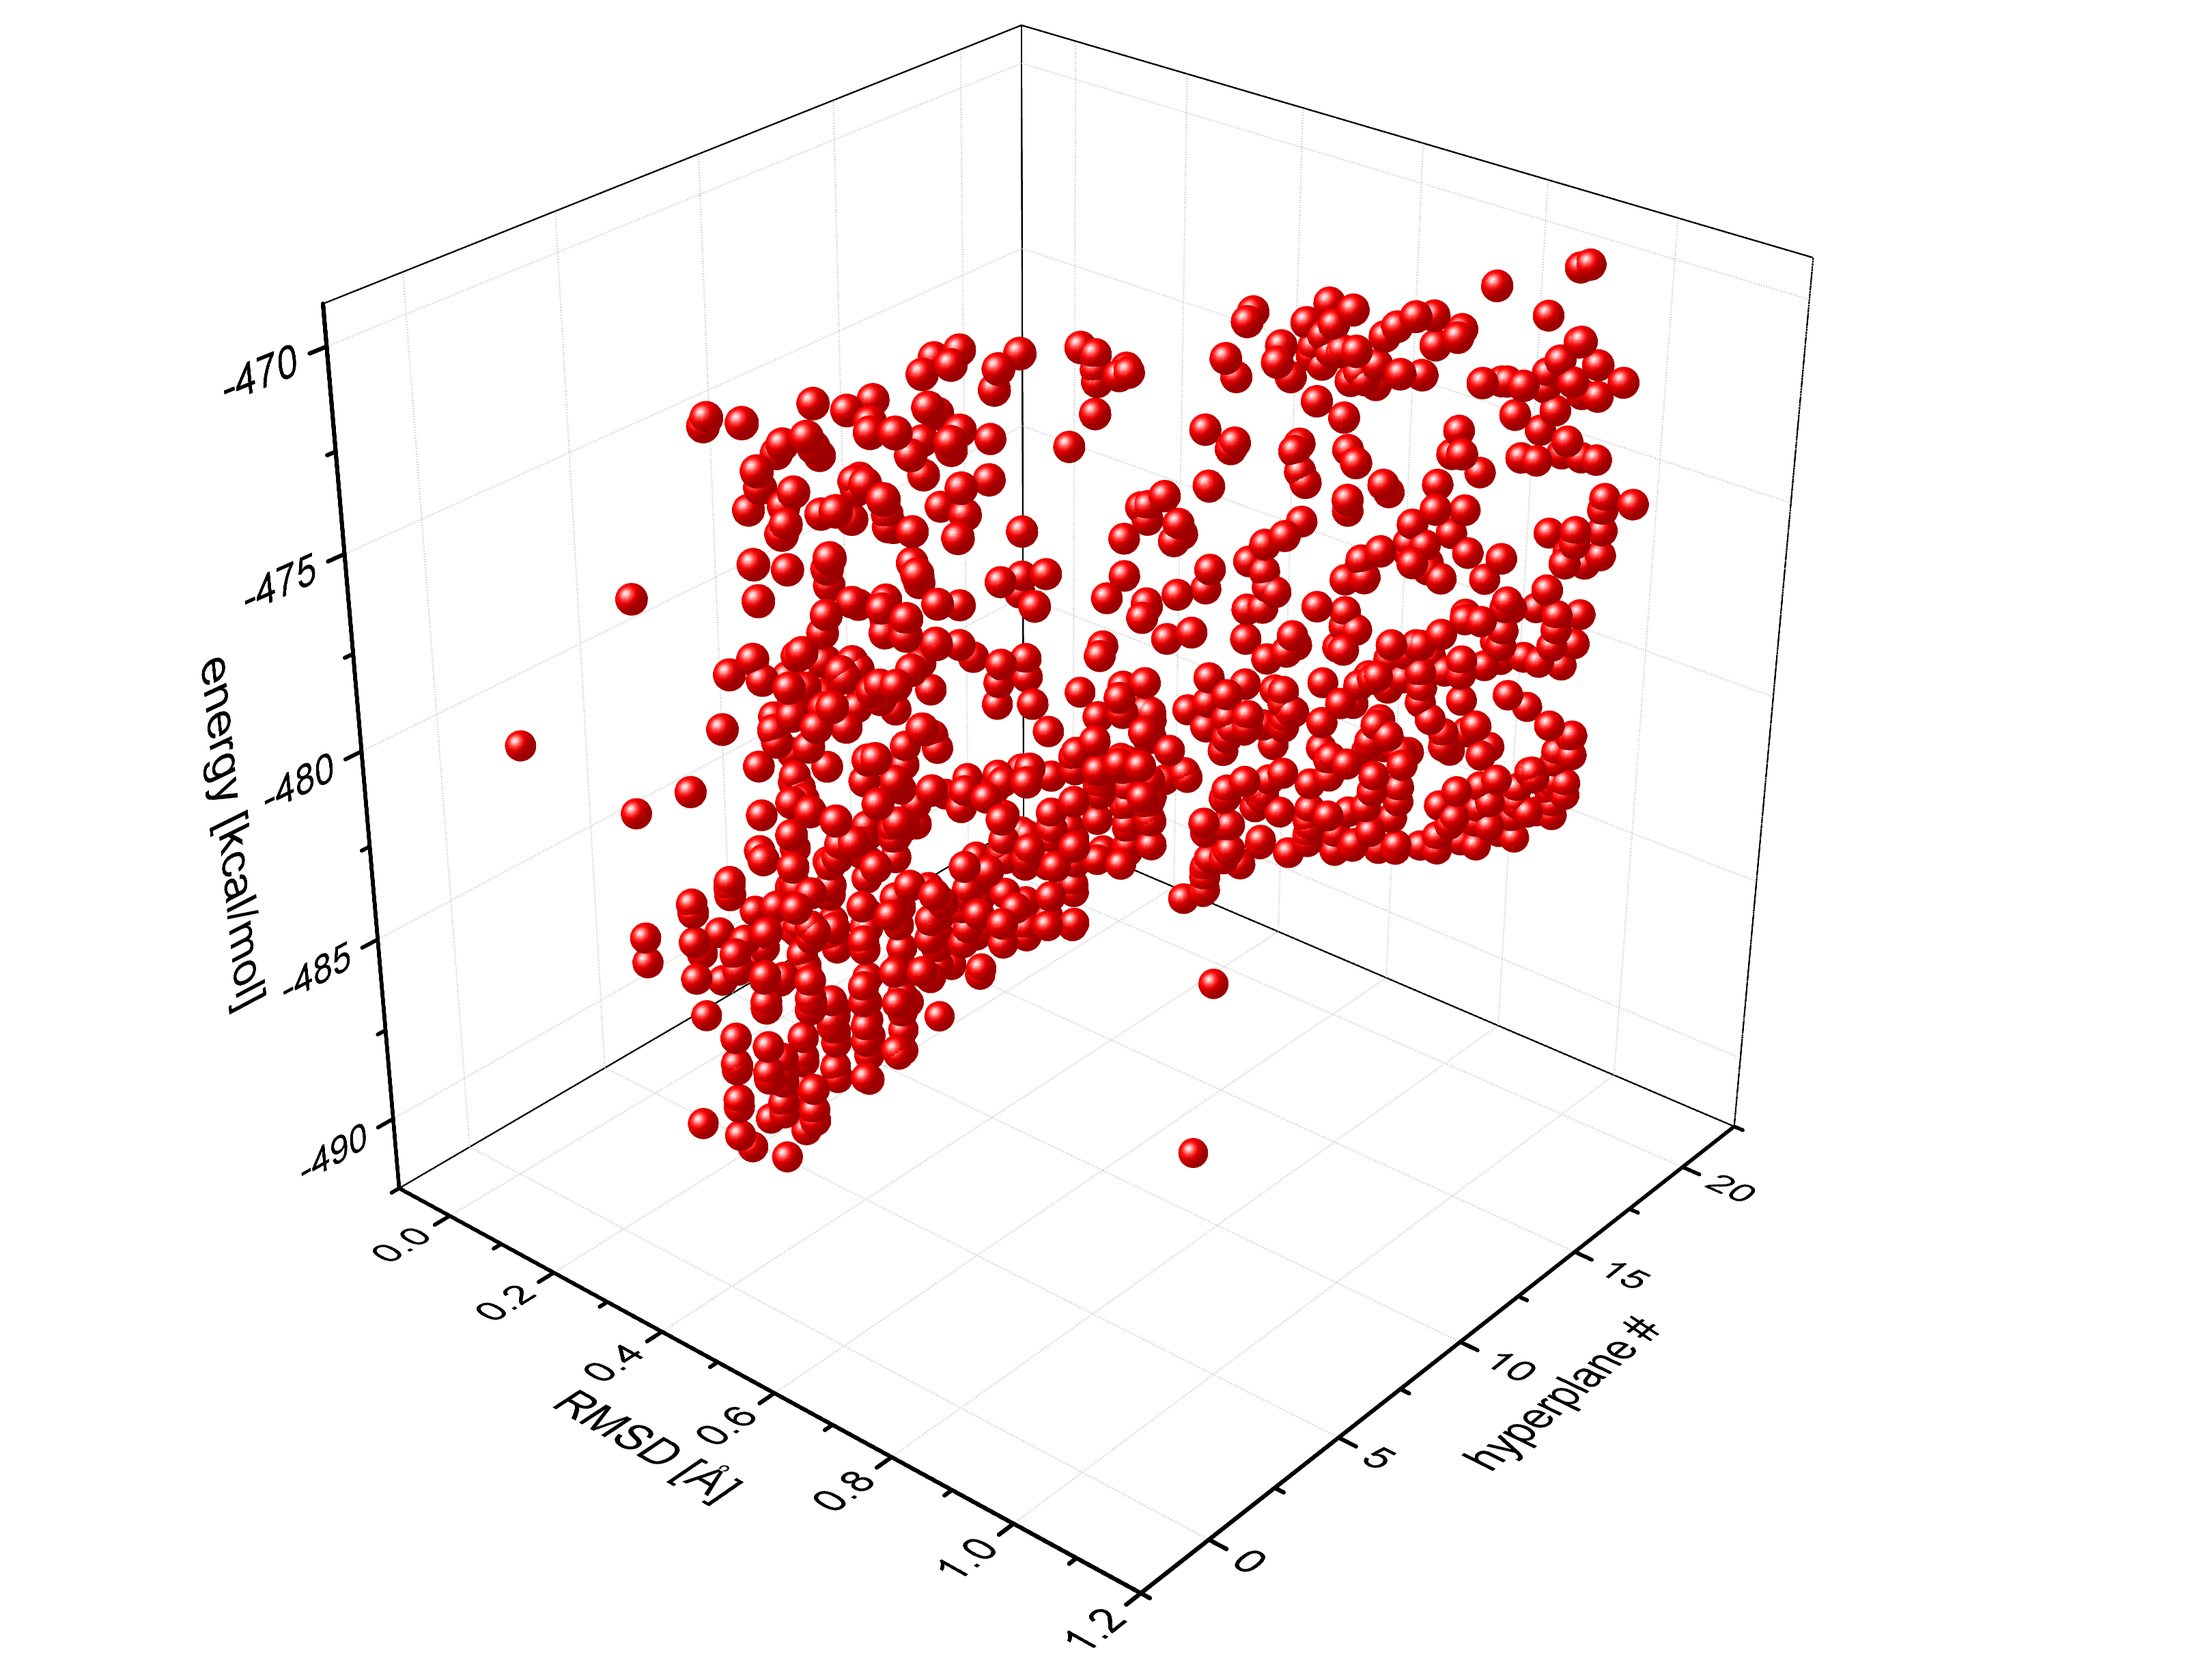
\includegraphics[scale=0.4]{Pathopt/trideca_energies.png}\caption{Distribution of found minima along the hyperplanes. The RMSD values are referenced to frame 0 on hyperplane 1.}
\label{fig:tridecaenergy}
\end{figure}

The next example is the alanine-glycine dipeptide molecule. For the dipeptide two structures (given in the Appendix) should be connected via NEB  or PO which are a little problematic. Within the FF description and the NEB method no reasonable pathway is found due to convergence failures which stem from the energy description. The initial an the final structure posses zwitterionic character and the linear transition from one to another structure leads to configurations which are not favorable within the zwitterionic FF description. One way two circumvent this failure is to use a QM description. A different way would be to carry out an PO optimization.  

\begin{figure}[H]
		\center
		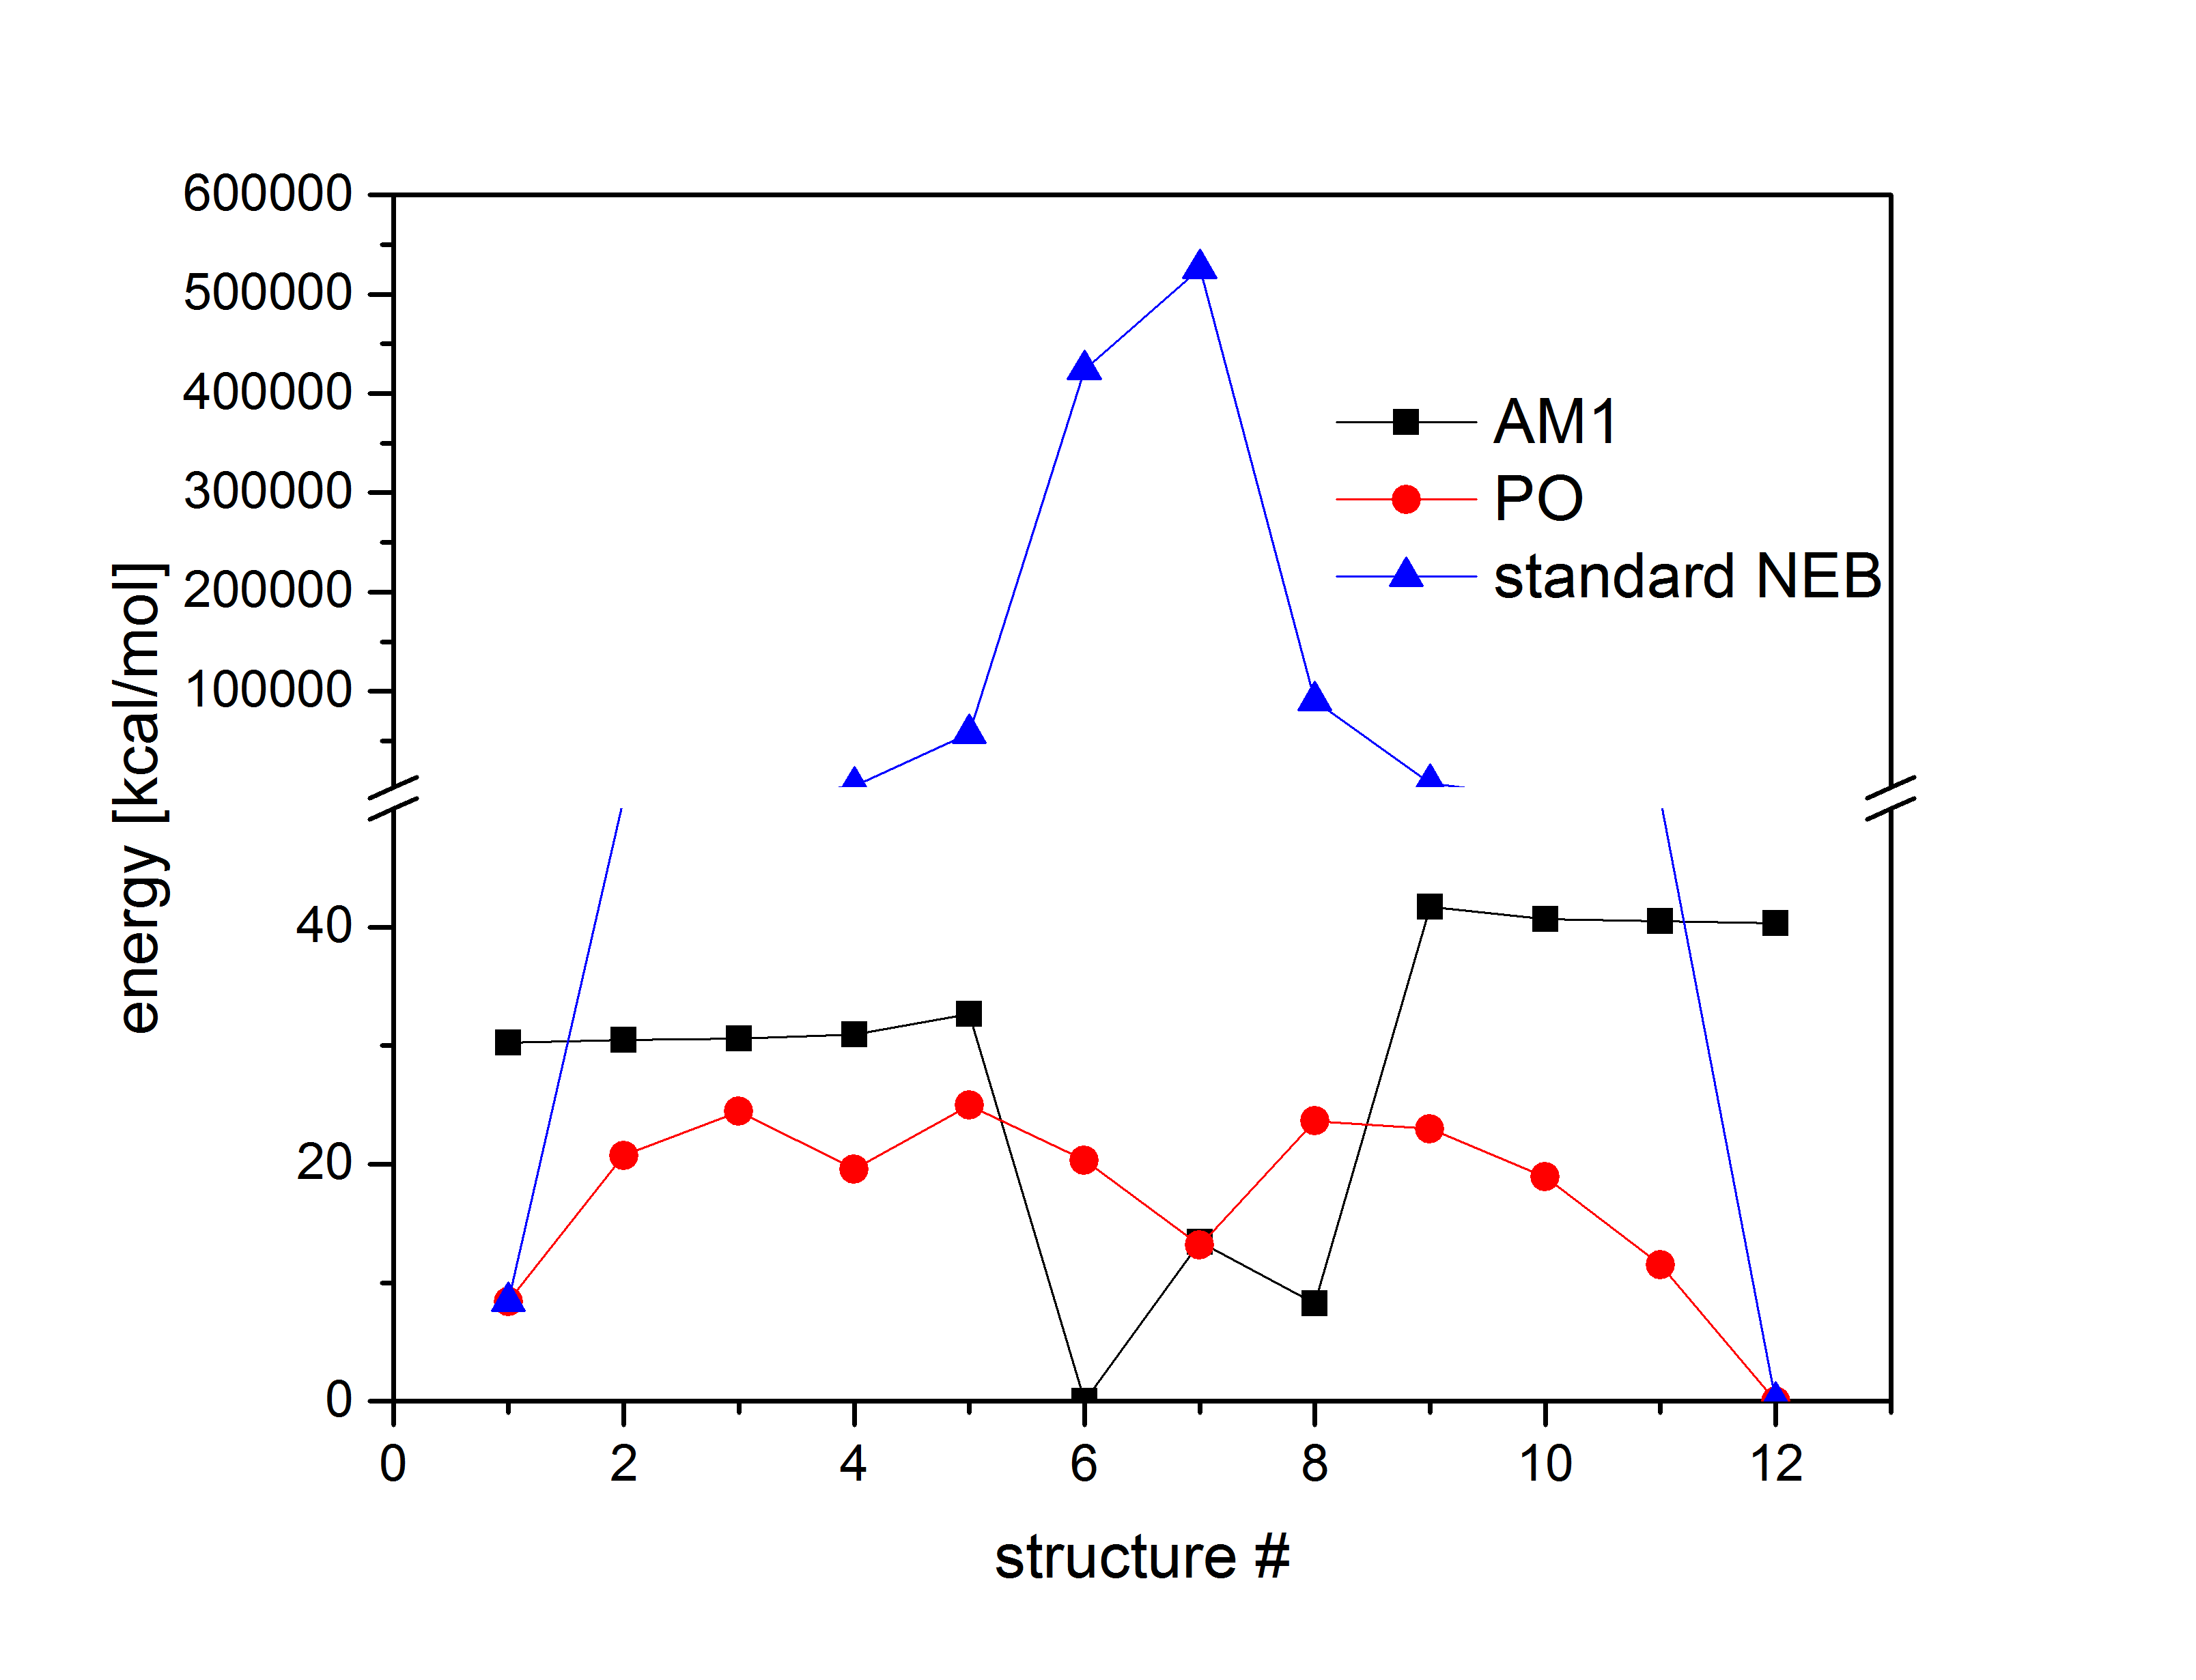
\includegraphics[scale=0.4]{Pathopt/PO_NEB_alagly_vergl.png}\caption{The figure shows the not converged NEB pathway (blue) which is obtained by using standard parameters and the OPLS-AA FF description. In red, one of the PO pathways (OPLS-AA) is depicted and in black the NEB pathway by using the AM1 energy description.}
\label{fig:POalaglypaths}
\end{figure}

\begin{figure}[H]
		\center
		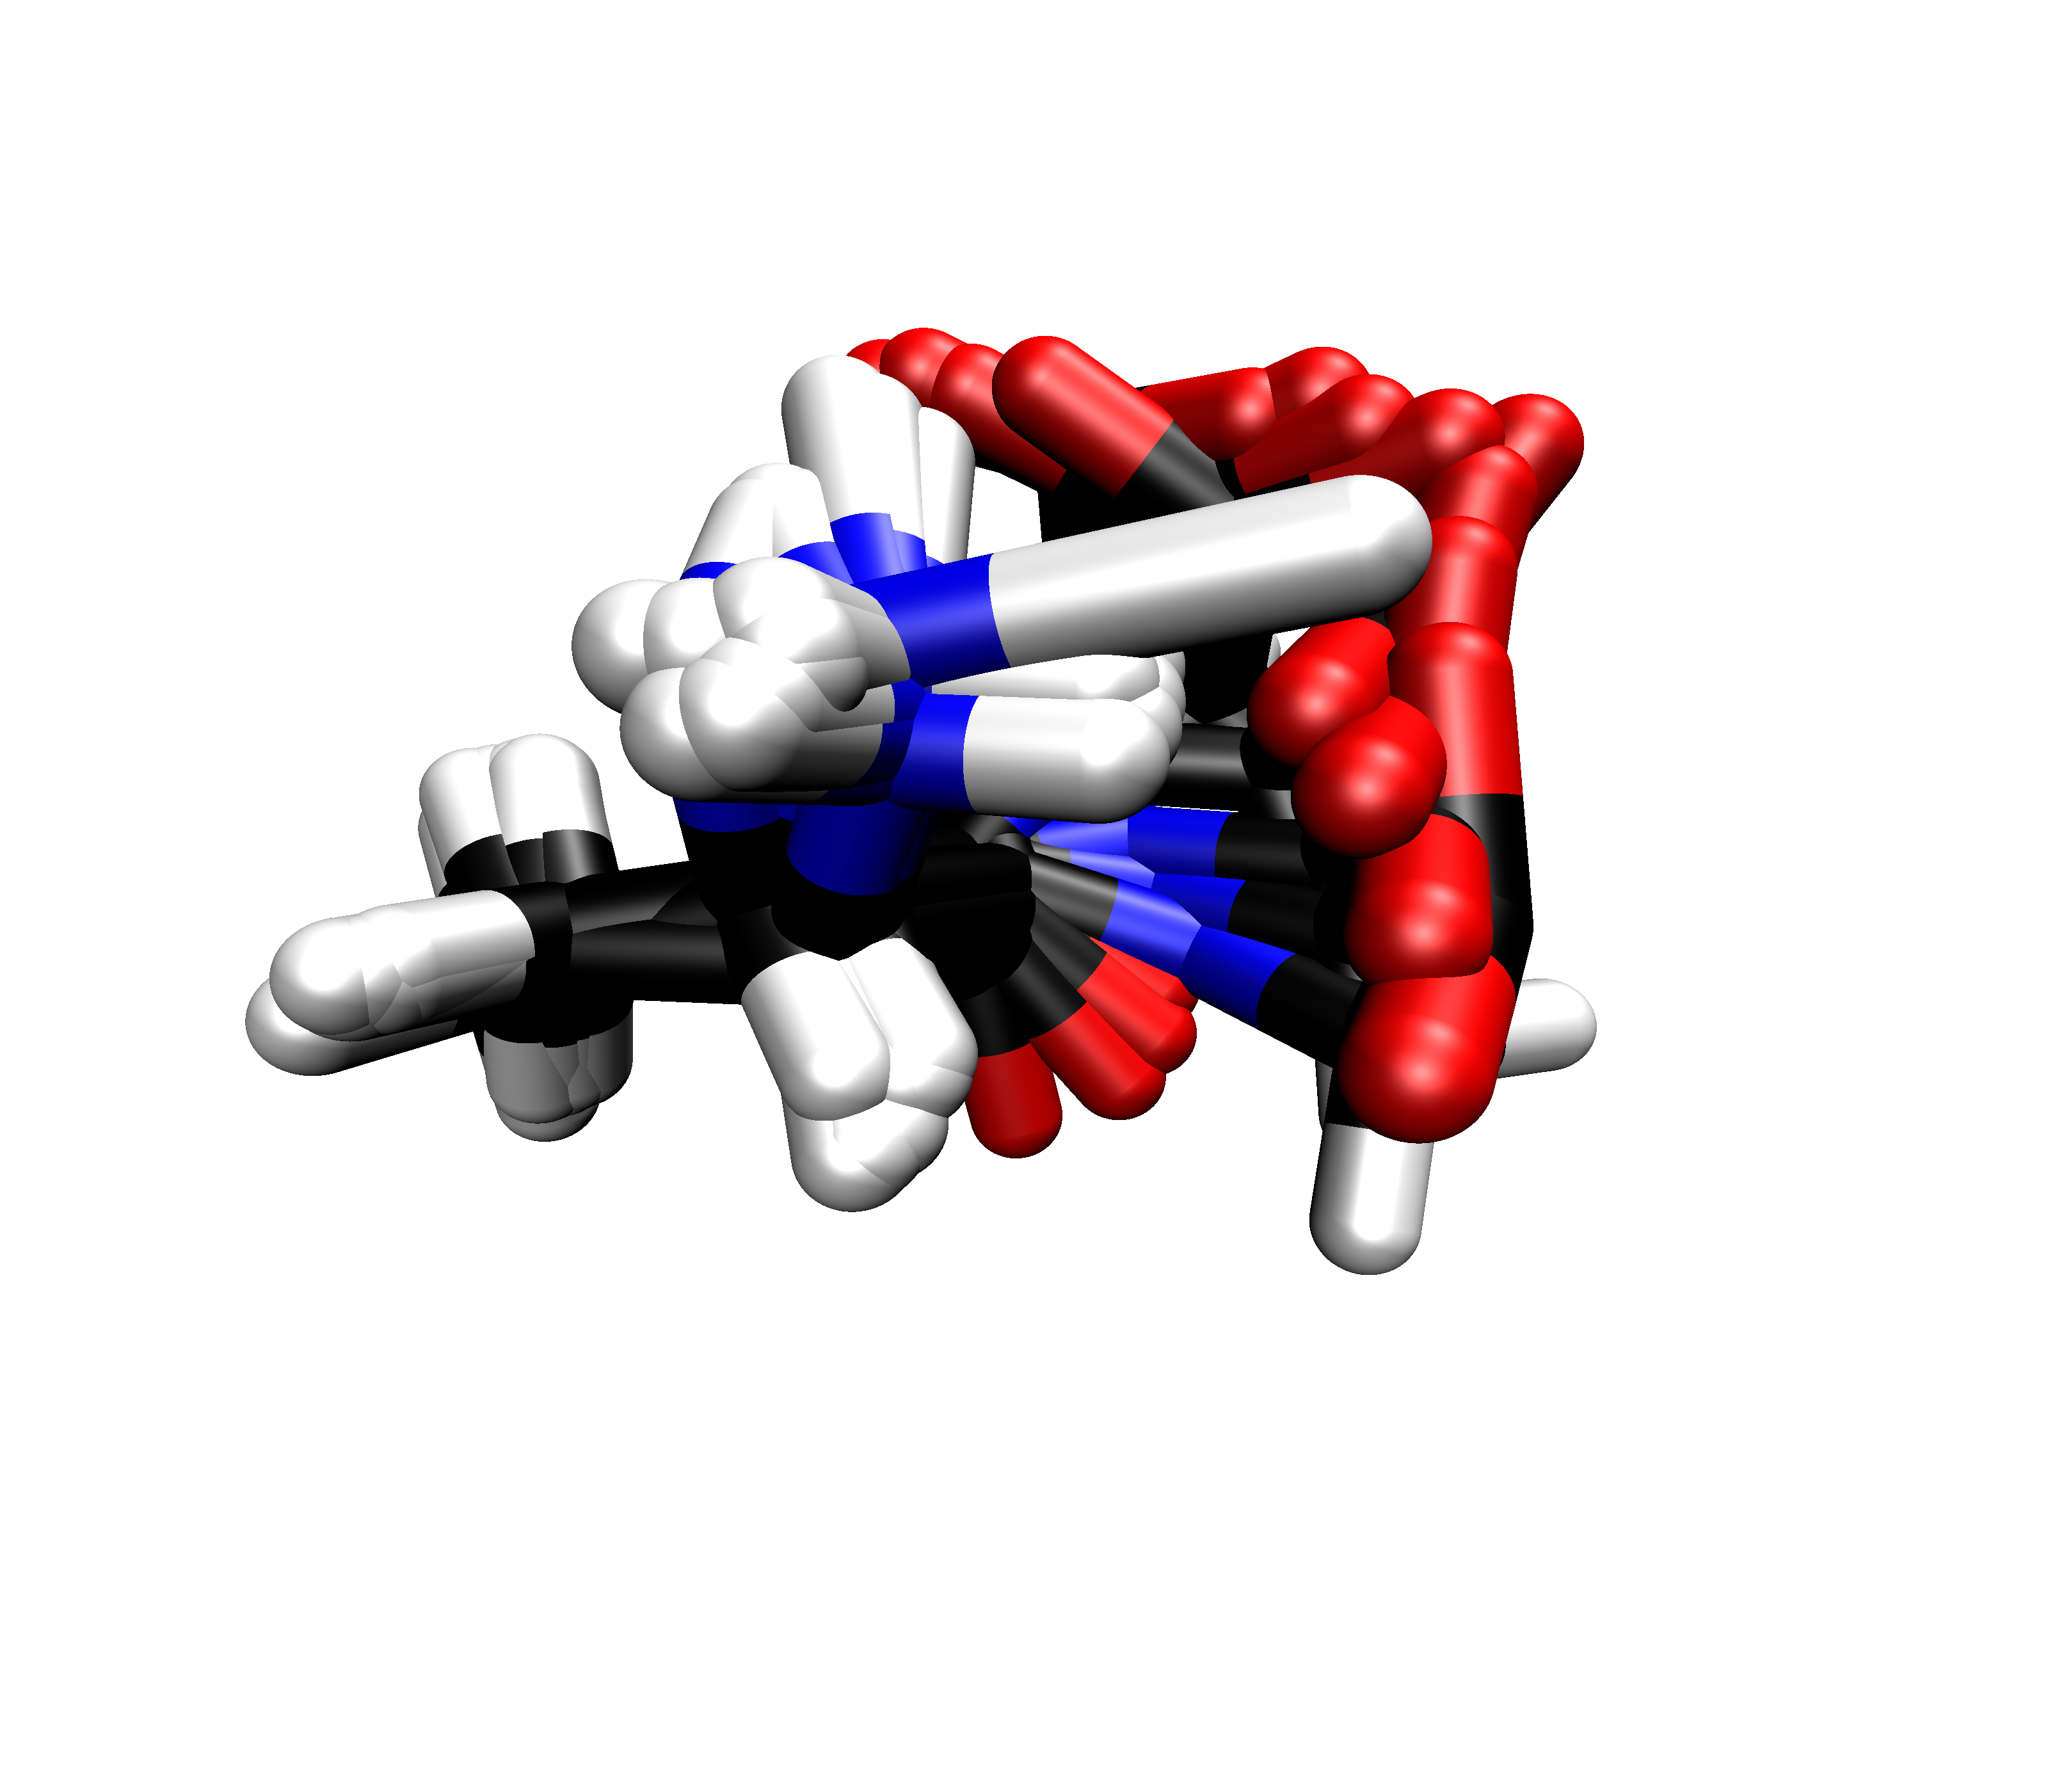
\includegraphics[scale=0.1]{Pathopt/ala_gly_am1_pathway.png}\caption{The structures which form the AM1 NEB pathway are given.}
\label{fig:POalaglystrucam}
\end{figure}

\begin{figure}[H]
		\center
		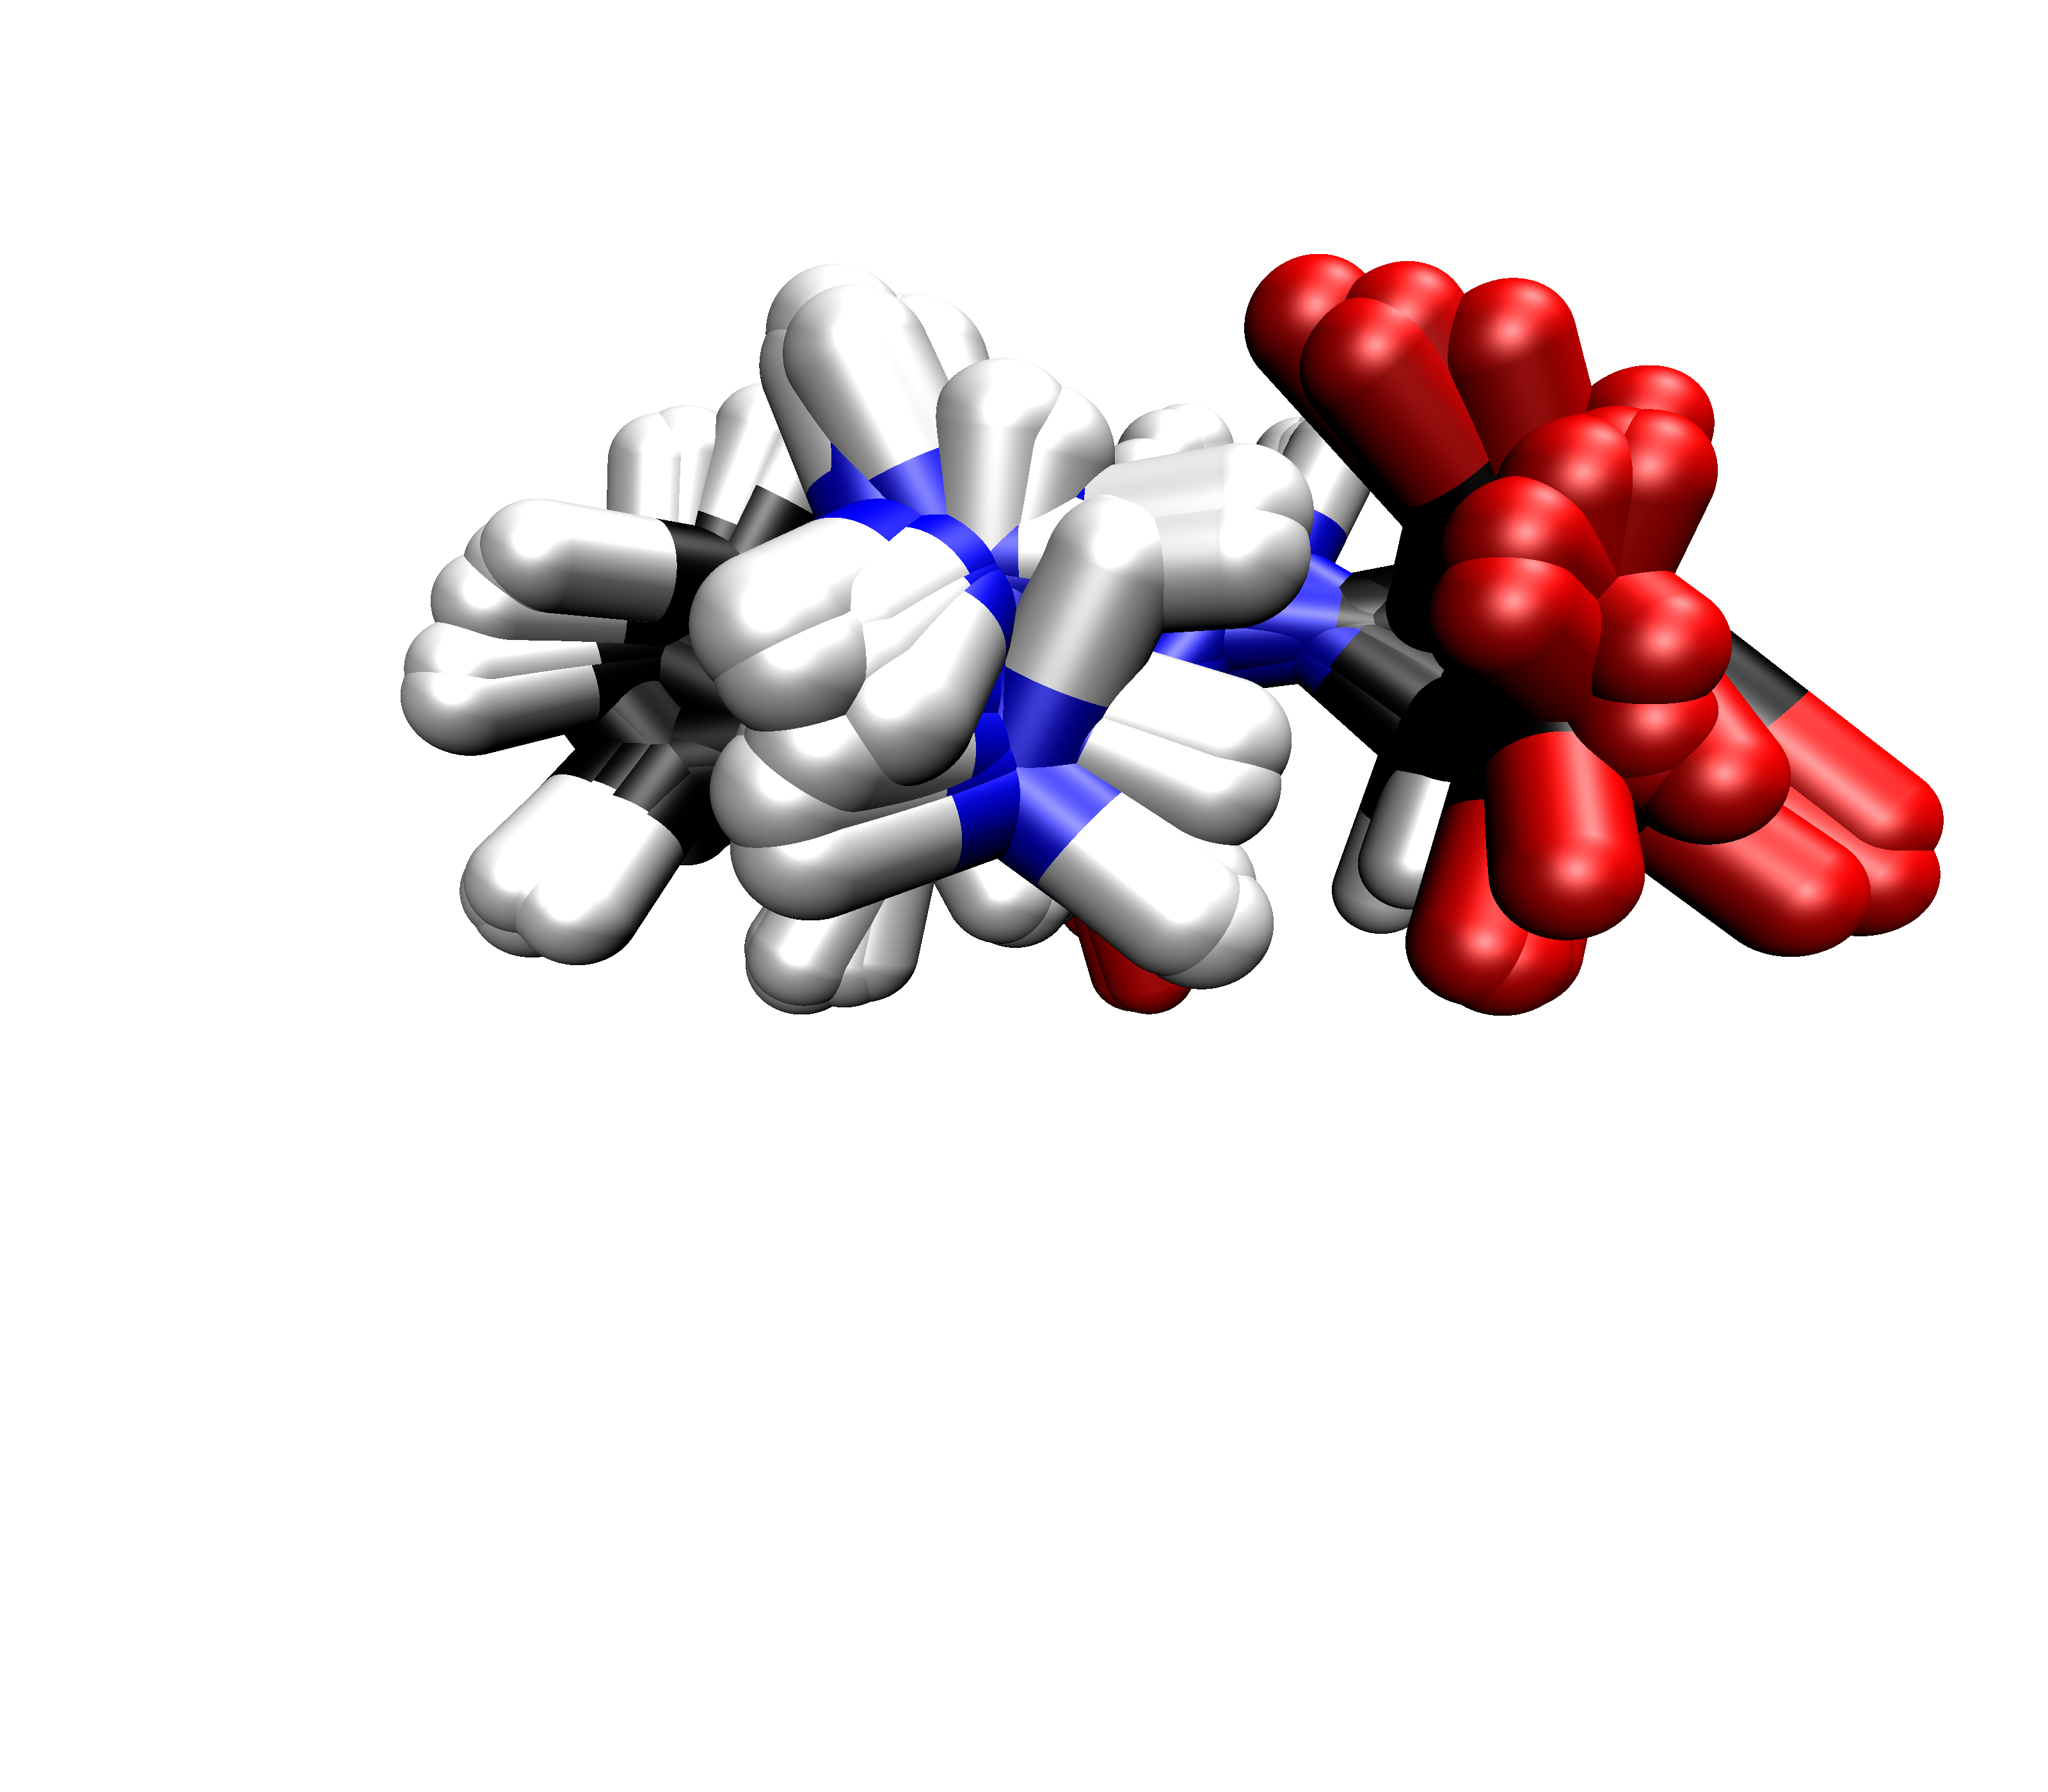
\includegraphics[scale=0.1]{Pathopt/PO_gly_ala_1.png}\caption{The structures which form the PO pathway built upon the OPLS-AA description are given.}
\label{fig:POalaglystrucpo}
\end{figure}
In this case it was possible to create a different pathway by varying the energy description and in addition PO shows the capability to find pathways around the initial linear pathway within the same FF description. In figure \ref{fig:POalaglypaths} the AM1 pathway structures show that the abstraction of the proton from the ammonium group (positively charged) and attach it to the carboxylate (negatively charged) is more stable along the linear pathway. 

\newpage

\printacronyms[include-classes=abbrev,name=Abbreviations]

\newpage

\printbibliography

\newpage

\appendix
\section{\texttt{AlaGly.xyz}}
\label{app:alaglytinker}
\begin{lstlisting}[
basicstyle=\footnotesize,
escapeinside={(@*}{*@)},
frame=single,
numbers=left,
]
          20  
 1  N3    -0.679000    1.176000   -0.480000    230   2  12   6  13
 2  CT     0.000000   -0.000000    0.000000    774   1   3   7   8
 3  C     -0.684000   -1.184000   -0.483000    177   2   5   4
 4  N     -2.062000   -1.412000   -0.135000    180  14   3  18
 5  O     -0.267000   -2.292000   -0.189000    178   3
 6  H3    -1.629001    1.176004   -0.144002    233   1
 7  CH     0.000000    0.000000    1.450000     80   2   9  10  11
 8  HC     1.027000    0.000000   -0.363000    892   2
 9  HC    -1.027000    0.000000    1.813000     85   7
10  HC     0.513000   -0.889000    1.813000     85   7
11  HC     0.513000    0.889000    1.813000     85   7
12  H3    -0.679000    1.176000   -1.488000    233   1
13  H3    -0.203783    1.999027   -0.144054    233   1
14  C     -2.510000   -2.644000   -0.731000    186   4  15  19  20
15  C     -2.384000   -2.557000   -2.173000    213  14  17  16
16  O2    -1.885000   -1.390000   -2.763000    214  15
17  O2    -2.712000   -3.502000   -2.872000    214  15
18  H     -2.150000   -1.472000    0.867000    183   4
19  HC    -3.553000   -2.816000   -0.468000    741  14
20  HC    -1.902000   -3.468000   -0.362000    741  14
\end{lstlisting}

\section{\texttt{AlaGly\_final\_LOCOPT.arc}}
\label{app:finalarc}
\begin{lstlisting}[
basicstyle=\footnotesize,
escapeinside={(@*}{*@)},
frame=single,
numbers=left,
]
20
 1  N3    -0.716463    0.459942   -0.932396   230     2     6    12    13
 2  CT     0.014710   -0.225311    0.153634   774     1     3     7     8
 3  C     -0.226806   -1.731938    0.013408   177     2     4     5
 4  N     -1.484582   -2.148443    0.200041   180     3    14    18
 5  O      0.667603   -2.452458   -0.411433   178     3
 6  H3    -0.585983    1.450174   -1.006646   233     1
 7  CH    -0.392379    0.309041    1.539094    80     2     9    10    11
 8  HC     1.082733   -0.056052    0.005354   892     2
 9  HC    -1.467155    0.226887    1.710368    85     7
10  HC     0.109266   -0.246858    2.333236    85     7
11  HC    -0.118419    1.357731    1.656718    85     7
12  H3    -1.723112    0.228853   -0.862306   233     1
13  H3    -0.533031   -0.013551   -1.815384   233     1
14  C     -2.225781   -2.763760   -0.896804   186     4    15    19    20
15  C     -2.703848   -1.535683   -1.677994   213    14    16    17
16  O2    -3.158228   -0.607857   -0.961833   214    15
17  O2    -2.018062   -1.231682   -2.673249   214    15
18  H     -2.114284   -1.484003    0.632037   183     4
19  HC    -3.077660   -3.334666   -0.528435   741    14
20  HC    -1.602043   -3.410428   -1.516725   741    14
\end{lstlisting}


\section{\texttt{CAST.txt}}
\label{app:casttxt}

\begin{lstlisting}[
basicstyle=\footnotesize,
escapeinside={(@*}{*@)},
frame=single,
numbers=left,
]
####################################
#                                  #
#                                  #
#         CAST CONFIGFILE          #(@*\label{appCAST:castconf}*@)
#                                  #
#                                  #
#################################### 

# Verbosity 
# Amount of output information from CAST [0-5] (do not use verbosity > 4 :-)

verbosity              4(@*\label{appCAST:verbosity}*@)

# Cores
# Number of OpenMP Threads (if compiled with openmp support)

cores                  4(@*\label{appCAST:cores}*@)


####################################
#                                  #
#                                  #
#        I/O: FILES & TYPES        #(@*\label{appCAST:filestypes}*@)
#                                  #
#                                  #
####################################

# Input file name

name                   AlaGly.xyz(@*\label{appCAST:filename}*@)

# Output file name

outname                AlaGly_final(@*\label{appCAST:output}*@)

# Input file type

inputtype              TINKER(@*\label{appCAST:intype}*@)

### AMBER I/O OPTIONS

#amber_mdcrd            min.rst
#amber_mdvel
#amber_inpcrd
#amber_restrt
#amber_trajectory_at_constant_pressure



#################################### 
#                                  #
#          PROGRAM TASK            #(@*\label{appCAST:tasks}*@)
#                                  #
####################################

# SP                   Single point eneryg calculation
# GRAD                 Single point energy calculation
# LOCOPT               Local optimization using Lib-LBFGS
# MD                   Molecular dynamics simulation
# GOSOL                Combined Solvation + Global Optimization
# MC                   Monte Carlo
# CENTER               Center of mass/geometry
# TS                   Tabu Search (CAST: GOTS)
# RMSD                 Root mean square deviation
# DIMER                Dimer method using torsional space
# NEB                  Nudged elastic band calculation
# INTERNAL             Create Z-Matrix
# STARTOPT
# UMBRELLA             Umbrella Sampling
# PROFILE              Repeated Gradient Calculation of first input structure
# FEP                  Alchemical transformations using FEP
# ALIGN                Trajectory Alignment (Kabsch algorithm)
# PCAgen               Principal Component Analysis
# PCAproc
# ENTROPY              Configurational and Conformational Entropy Calculations
# GRID                 Grid Search
# PATHOPT              Global reaction path search by constraint optimization on n-1 dim.
#                      hyperplane(s)
# ADJUST
# GRID
# PATHSAMPLING
# REMOVE_EXPLICIT_WATER

task                  LOCOPT(@*\label{appCAST:task}*@)


####################################
#                                  #
#        ENERGY INTERFACES         #(@*\label{appCAST:interfaces}*@)
#                                  #
####################################

# AMBER                AMBER force field
# (AMOEBA)             AMOEBA03 force field
# CHARMM22             CHARMM22 force field
# OPLS-AA               OPLS all atoms force field
# TERACHEM             Terachem MPI Interface
# (TINKER)             Tinker syscall interface
# MOPAC                MOAPC2012 syscall Interface

interface              OPLS-AA(@*\label{appCAST:interface}*@)

# Interface for preoptimizations

preinterface           0(@*\label{appCAST:preinterface}*@)

# PARAMETER FILE FOR forcefield
# paramfile            amber.prm, amoeba.prm, OPLS-AA.prm, charmm22.prm

paramfile              OPLS-AA.prm(@*\label{appCAST:paramfile}*@)

# Keywords for MOPAC Call

MOPACkey               PM7(@*\label{appCAST:mopaccall}*@)

# Delete temporary MOPAC comm files?

MOPACdelete            1(@*\label{appCAST:mopacdelete}*@)

#MOPAC executable path

MOPACpath              "C:\Program Files\mopac\MOPAC2012.exe"(@*\label{appCAST:mopacpath}*@)

#MOPACversion

# Short-range electrostatics correction 0/1 activate interpolative energies/gradients (0/1) and cutoff n.nn

Spackman 1 1 10.0 (@*\label{appCAST:spack}*@)

####################################
#                                  #
#          CUTOFF RADIUS           #
#                                  #
####################################

cutoff                 400.0
switchdist             10.0


####################################
#                                  #
#          ATOM FIXATIONS          #
#                                  #
####################################

# Exclude nonbondeds between two fixed atoms in internal force fields

FIXexclude             0

# Remove rotations of hydrogens from main torsional angles

REMOVEHROT             0

# Fix a range of atoms 
#FIXrange               <start index> <end index>

#FIXrange               1 213

# Fixation of single atoms
#ATOMFIX                <INDEX> 

#ATOMFIX                1
#ATOMFIX                3


####################################
#                                  #
#          Boundary Bias           #
#                                  #
####################################

# Quadratic Dihedral Bias Potential
#BIASspherical                <radius> <force> <exponent>
#BIAScubic                    <x> <y> <z> <force> <exponent>

#BIASspherical  25.0 1.0 2.0
#BIAScubic 40.0 40.0 40.0 1.0 2.0


####################################
#                                  #
#        DIHEDRAL FIXATIONS        #
#                                  #
####################################

# Quadratic Dihedral Bias Potential (quadratic in degreees)

#BIASdih                <atom 1> <atom 2> <atom 3> <atom 4> <angle> <force> <all atoms> 

#BIASdih                1 2 3 5 0.0   10.0 1
#BIASdih                2 5 6 9 150.0 5.0  1
#BIASdih                1 2 5 6 150.0 5.0  1 
#BIASdih                1 2 5 6 95.0  10.0 1

#BIASdih                1 2 5 6 60.0 0.01

#BIASdih                1 2 5 6 30.0 1.0 1



####################################
#                                  #
#             MAINlists            #
#                                  #
####################################

# Black- or Whitelist a rotation around a bond
# for the selection as main rotation

#MAINblacklist 2 5

#MAINwhitelist 2 5


####################################
#                                  #
#       Periodic Boundaries        #
#                                  #
####################################

#Periodics            <Active 1(on)/0(off)> <box-x> <box-y> <box-z>
#Periodics              0 70.0 70.0 70.0

# Print periodic boundary dummy atoms to output?
#Periodicp            <Active 1(on)/0(off)> 

#Periodicp              0


####################################
#                                  #
#        INTERACTION OPTIONS       #
#                                  #
####################################

# The interaction of substructures that are not bound to each other can be calculated
# IAlimits <Start Index Substructure> <End Index Substructure>

#IAlimits               1 122



####################################
#                                  #
#        Implicit Solvation        #
#                                  #
####################################

# solvmethod : VAC         (default) Vacuum
#              ONION       Numerical Still method
#              STILL       Analytical Still method
#              HCT         HCT method
#              OBC         OBC method
#              GRYCUK      Grycuk's method
#              ACE         ACE method
# surface    : TINKER      (default) TINKER's accessible surface area calculation
#              SASASTILL   Still's surface area calculation
#              GAUSS       SASA according to the global theorem of Gauss-Bonnet
#
# ONION should only be combined with GAUSS

solvmethod             VAC
surface                TINKER


#################################### 
#                                  #
#        PROFILE RUNS              #
#                                  #
####################################

# Number of repeated gradient calculations for PROFILE task

profileruns            10


####################################
#                                  #
#         libLBFGS OPTIONS         #
#                                  #
####################################

BFGSgrad               0.0001 (@*\label{appCAST:bfgsgrad}*@)
BFGSmaxstep            5000 (@*\label{appCAST:bfgsstep}*@)


###################################
#				  												#
#      NEB & 											#(@*\label{appCAST:neb}*@)
#			 PATHOPT OPTIONS      			#(@*\label{appCAST:pathopt}*@)
#				 													#
###################################

# Second structure for double-ended search
NEB-PATHOPT-FINAL input.xyz(@*\label{appCAST:nebfinal}*@)

# Number of NEB images
NEB-PATHOPT-IMAGES 12(@*\label{appCAST:nebimages}*@)

# Force constant in kcal/molA^2 for NEB calculation defining the force component along the
# connecting band
NEB-PATHOPT-SPRING 1.0(@*\label{appCAST:nebspring}*@)

# Climbing image in NEB 0/1 (off/on)
NEB-PATHOPT-CLIMBING 1(@*\label{appCAST:nebclimbing}*@)

# Standard tau or improved tau method in NEB 0/1 (standard/improved)
NEB-PATHOPT-TAU 1(@*\label{appCAST:nebtau}*@)

# Definition of the Temperature settings for the Monte Carlo run
NEB-PATHOPT-TEMP 298.15(@*\label{appCAST:nebtemp}*@)

# MCM iterations in Pathopt
NEB-PATHOPT-ITER 60(@*\label{appCAST:nebiter}*@)

# Number of multiple MCM simulations
NEB-PATHOPT-GLOBITER 1(@*\label{appCAST:nebglobiter}*@)

# Optimization mode BIAS/GRADIENT Projection
NEB-PATHOPT-MODE PROJECTED(@*\label{appCAST:nebmode}*@)

# Bias constant (Pathopt)
NEB-PATHOPT-BIASCONSTANT 0.1(@*\label{appCAST:nebbiasconstant}*@)

# Maximum displacement in Angstrom for accepted coordinates in MCM 
NEB-PATHOPT-MAXVAR 3.0(@*\label{appCAST:nebmaxvar}*@)

# Maximum energy range in kcal/mol for MCM in Pathopt
NEB-PATHOPT-ENERGY_RANGE 20.0(@*\label{appCAST:nebenergyrange}*@)

# MCM stepsize in Angstrom
NEB-PATHOPT-STEPSIZE 1.4(@*\label{appCAST:nebstepsize}*@)

# Move strategy by applying dihedral changes at several steps of MCM 0/1 (off/on)
NEB-PATHOPT-MIXMOVE 0(@*\label{appCAST:nebmixmove}*@)

# Using NEB connection within Pathopt 0/1 (off/on) 
NEB-PATHOPT-NEBCONN 0(@*\label{appCAST:nebnebconn}*@)

# Number of NEB images within Pathopt-NEB connection procedure
NEB-PATHOPT-NEBCONN_NUMBER 12(@*\label{appCAST:nebnebconnnumber}*@)

# Constraint global optimization (MCM standard) by fixation of
# dihedrals which change the most during NEB
NEB-PATHOPT-CONSTRAINT_GLOBAL 0(@*\label{appCAST:nebconstraintglobal}*@)

# Number of dihedrals within constraint global optimization 
# (MCM standard) which should be fixed along the NEB path
NEB-PATHOPT-CONSTRAINT_NUMBER_DIHEDRALS 1(@*\label{appCAST:nebnumberdihedrals}*@)

# Interpolation via spline method between the linear constructed NEB pathway
# by locally optimizing with perpendicular force projection 0/1 (off/on) 
NEB-PATHOPT-INT_PATH 0(@*\label{appCAST:nebintpath}*@)

#step size of interpolated images via spline interpolation approach
NEB-PATHOPT-INT_IT 0.5(@*\label{appCAST:nebintit}*@)

# choose if the MaxFlux method is used to simulate a NEB method with temperature dependencies 
# (0/1 no/yes)
NEB-PATHOPT-MAXFLUX 1(@*\label{appCAST:nebmaxflux}*@)

# determine if a neb calculation is performed for every found path in PATHOPT (0/1: no/yes)
NEB-PATHOPT-MF_PATHOPT 1(@*\label{appCAST:nebmfpathopt}*@)

# image dependent pair potential approach for generation of initial pathway in NEB optimization
# (0/1: no/yes)
NEB-PATHOPT-NEB-IDPP 1(@*\label{appCAST:nebidpp}*@)

# complete pathway NEB calculation (0/1: no/yes)
NEB-PATHOPT-NEB-COMPLETE 1(@*\label{appCAST:nebcomplete}*@)

####################################
#                                  #
#        SIMULATION OPTIONS        #(@*\label{appCAST:mcts}*@)
#            (MC, TS)              #
#                                  #
####################################

# Simulation Temperature 
# for TS and MC important for Metropolis Criterion

Temperature            298.15(@*\label{appCAST:mctstemperature}*@)

# Number of iterations in global optimization routine 

Iterations             2000(@*\label{appCAST:mctsiterations}*@)


####################################
#                                  #
#           GLOBOPTIONS            #
#            (MC, TS)              #
#                                  #
####################################

# Save all (minimized) structures 
# which are within "Erange" kcal/mol from the final global minimum
# default = 0.0

GOerange                 10.0(@*\label{appCAST:goerange}*@)

# use the current local minimum energy for metropolis criterion?
# default = 0

GOmetrolocal           0(@*\label{appCAST:gometrolocal}*@)

# startopt before starting simulation/optimization?
# default = 0

GOstartopt             0(@*\label{appCAST:gostartopt}*@)

# Temperature Scaling Factor applied to the Temperature, 
# once a new minimum is found during GlobOpt
# default = 1.0

Tempscale              1.0(@*\label{appCAST:gotempscale}*@)

# Precision of values printed

GOprecision            6(@*\label{appCAST:goprecision}*@)

# Fallback type 
# 
# LAST_GLOBAL (default) = fall back to last minimum and then to global minimum if stuck
# EVOLUTION = select new minimum via evolutionary algorithm if stuck

GOfallback             LAST_GLOBAL(@*\label{appCAST:gofallback}*@)

# Maximum number of tries from one structure before it is set
# tabu as a starting point
# default = 20

GOfallback_limit       500(@*\label{appCAST:gofallbacklimit}*@)

# Fitness function type for evolutionary fallback
#
# LINEAR (default) = linear ranking
# EXPONENTIAL = exponential ranking

GOfallback_fr_fit              EXPONENTIAL(@*\label{appCAST:gofallbackfrfit}*@)

# Number of minima included in the ranking for evolutionary fallback
# default = 10

GOfallback_fr_minima    10(@*\label{appCAST:gofallbackfrminima}*@)

# Lower and upper bounardy for fitness value
# rank 1 is assign second value, rank X 
# (determined via GOincluded_minima) is assigned the first value
# default = 0.5 1.0

GOfallback_fr_bounds       0.5 1.0(@*\label{appCAST:gofallbackfrbounds}*@)


####################################
#                                  #
#           GRID OPTIONS           #
#                                  #
####################################

GOmain_grid            60.0(@*\label{appCAST:gomaingrid}*@)


####################################
#                                  #
#            MCM OPTIONS           #
#                                  #
####################################

# Step size in cartesian space 

MCstep_size            1.4(@*\label{appCAST:mcstepsize}*@)

# Use minimization

MCminimization         1(@*\label{appCAST:mcminimization}*@)

# Use dihedral (1), cartesian (2) or biased dihedral (0) randomization

MCmovetype             1(@*\label{appCAST:mcmovetype}*@)

# Maximum dihedral deviation

MCmax_dihedral         30.0(@*\label{appCAST:mcmaxdihedral}*@)


####################################
#                                  #
#            TS OPTIONS            #(@*\label{appCAST:ts}*@)
#                                  #
####################################

# Do diversification before first TS steps?

TSmc_first             0(@*\label{appCAST:tsmcfirst}*@)

# How many TS steps need to fail in finding new minimum before diversification?

TSdivers_threshold      10(@*\label{appCAST:tsdiversthreshold}*@)

# How many diversification steps are applied?

TSdivers_iter          30(@*\label{appCAST:tsdiversiter}*@)

# How often will diversification be applied before termination?

TSdivers_limit         20(@*\label{appCAST:tsdiverslimit}*@)


####################################
#                                  #
#         STARTOPT OPTIONS         #
#                                  #
####################################

# startopt type
# 0                  Ringsearch
# 1                  Solvadd [default]
# 2                  Ringsearch + Solvadd

SOtype                 1

# startopt structure count
# number of structures generated by startopt routines

SOstructures           10


####################################
#                                  #
#        RINGSEARCH OPTIONS        #
#                                  #
####################################

# Force, applied to close rings 
# (multiplied with quadratic in degrees of dihedral deviation)

RSbias_force           10.0

# Chance to close a ring in the initial random population generation

RSchance_close         0.33

# Number of individuals in the ringsearch evolution

RSpopulation           10

# Number of propagated generations during ringsearch evolution

RSgenerations          10


####################################
#                                  #
#          SOLVADD OPTIONS         #
#                                  #
####################################

# Hydrogen bond length parameter [default: 1.8]

SAhb                   1.8

# number of desired water molecules [default: 0(=no limit)]

SAlimit                20

# water boundary type
#
# 0    layer [default]
# 1    sphere
# 2    box

SAboundary             0

# water boundary extent [default: 10.0] and push length (elongation of radius if limit is
# not reached)

SAradius               10.0

# force field parameter types of oxygen and hydrogen
#
# 53 54   OPLS-AA
# 101 88   CHARMM
# 2001 2002  AMBER

SAtypes                53 54

# Intermediate optimizations
#
# 0    none
# 1    each "shell"
# 2    all waters
# 3    1+2

SAopt                  0

# fix initial structure

SAfixinit              1




####################################
#                                  #
#            MD OPTIONS            #(@*\label{appCAST:md}*@)
#                                  #
####################################

# Number of Steps

MDsteps                50000(@*\label{appCAST:mdsteps}*@)

# Integrator
#
# 0                    Velocity-Verlet
# 1                    Beeman

MDintegrator           0(@*\label{appCAST:mdintegrator}*@)

# Velocity Scaling

MDveloscale            1(@*\label{appCAST:mdveloscale}*@)

# Thermostat (Nose-Hoover)

MDthermostat           1(@*\label{appCAST:mdthermostat}*@)

# Timestep in picoseconds

MDtimestep             0.001(@*\label{appCAST:mdtimestep}*@)

# start MD again from beginning if molecule gets destroyed

MDrestart_if_broken    0(@*\label{appCAST:mdrestartifbroken}*@)

# Activate Tracking (Log and Snapshots)

MDtrack                1(@*\label{appCAST:mdtrack}*@)

#MDtrackoffset         0

#
#   Snapshots
#

# Number
MDsnap                 1000(@*\label{appCAST:mdsnap}*@)
# Buffer size
MDsnap_buffer          100(@*\label{appCAST:mdsnapbuffer}*@)
# Optimize snapshots
MDsnap_opt             0(@*\label{appCAST:mdsnapopt}*@)

# Heating process control
#
# MDheat               <step> <temperature at that step>(@*\label{appCAST:mdheat}*@)

MDheat                 0  298.15(@*\label{appCAST:mdheat1}*@)
MDheat                 10000  348.15(@*\label{appCAST:mdheat2}*@)
MDheat                 20000  398.15(@*\label{appCAST:mdheat3}*@)
MDheat                 30000  448.15(@*\label{appCAST:mdheat4}*@)
MDheat                 40000  498.15(@*\label{appCAST:mdheat5}*@)

# Pressure control

#MDpress               0(@*\label{appCAST:mdpress}*@)

#MDpcompress
#MDpdelay
#MDptarget

# Spehrical boundaries' options
# 
# MDspehrical          <Active 0/1> <Radius 1> <Radius 2> <Force 1> <Force 2> <Exp 1> <Exp 2>(@*\label{appCAST:mdspherical}*@)

#MDspherical            0 34.0 34.1 10.0 10.0 2.0 4.0

# H bond constraints
#
# 0                    No Constraints
# 1                    All Hydrogend Bonds
# 2                    Specific Hydrogen Bonds

MDrattle               0(@*\label{appCAST:mdrattle}*@)

#MDrattpar

# Rattle bond specification
#
# MDrattlebond         <H index>(@*\label{appCAST:mdrattlebond}*@)

#MDrattlebond           7 12

#apply a biased potential
#MDbiased potential        <0/1>

MDbiased_potential         0

#atom number(s) of active site <every atom a new line> 
#MDactive_site        1

#cutoff around active site <inner/outer>
#MDcutoff                1 2

#adjust active center + distances with every step
#MDadjust_by_step     <0/1>

MDadjust_by_step      1

# Iteration offset for restart files

MDrestart_offset       10000

# Resume simulation from restart file?

MDresume               0

#MDpre_optimize


####################################
#                                  #
#            FEP OPTIONS           #
#                                  #
####################################

FEPlambda      1.0
FEPdlambda     0.05
FEPvdwcouple   1.0
FEPeleccouple  0.5
FEPvshift      0.1
FEPcshift      2.0
FEPequil       100
FEPsteps       500
FEPfreq        1000


####################################
#                                  #
#            PATH OPTIONS          #
#                                  #
####################################

# File containing the desired path end

PRendfile              PATHREL_END.xyz

# Maximum Energy distance within the path

PRdeltae               0.5

# Maximum structure distance with the path

PRdeltax               0.5


####################################
#                                  #
#           DIMER OPTIONS          #
#                                  #
####################################
#
# Distance between dimer start end endpoint

DIMERdistance          0.001

# Maximum absolute of rotational force during dimer translation

DIMERtflimit           0.01

# Convergence criterion for the dimer rotation

DIMERrotconvergence    5.0

# Maximum number of rotation and translation iterations

DIMERmaxit             50 250



####################################
#                                  #
#         UMBRELLA SAMPLING        #
#                                  #
####################################


USsteps                60

# definition of strained torsion

#UStorsion              <index 1> <index 2> <index 3> <index 4> <force> <phi0>
#                       <flat bottom 0/1> <width>
#[int] 1-4              atom indices
#[float] force          potential force constant
#[float] phi0           start angle
#[float] phi1           ending angle
#[int] steps            number of sampling steps
#[bool/int]             switch to activate fixation of all torsions around the specified 

#UStorsion              1 2 5 6 100.0 180.0 120.0 1

# definition of strained bond

#USbond                 <index 1> <index 2> <force> <r0> <flat bottom 0/1> <width>
#USbond                 1 2 155.0 1.09 1 0.2

# Offset for taking snapshots

USsnap                 5


####################################
#                                  #
#              ADJUST              #
#                                  #
####################################


#ADJUSTdih 1 2 3 4 180.0
#ADJUSTdih 2 3 4 5 180.0


####################################
#                                  #
#   TRAJECTORY ALIGNMENT OPTIONS   #
#                                  #
####################################

# Should alignment be performed?
traj_align_bool                true
# Should distance meassures be calculated and printed?
traj_print_bool                false


# Should we align to an external reference structure? If yes, give file name
align_external_file            reference.xyz

# Reference frame for alignment (using Kabsch algorithm)
# default is "0"
ref_frame_num                   110


# Desired distance masurement unit for output
# 0: RMSD (default)
# 1: dRMSD
# 2: Hold and Sander Score

dist_unit                       0

# if Holm and Sander Score is chosen, pick value for r_c
# (contact cutoff distance)
# default is "20", as in original publication

holm_sand_r0                    5


####################################
#                                  #
#       ENTROPY-CALC OPTIONS   	   #
#                                  #
####################################

# Should alignment (Kabsch algorithm, minimizes RMSD) be performed
# prior to calculations? (options: false / true; true is default)
# entropy_ref_frame_num gives reference frame for alignment (default is 0)
entropy_alignment                 true
entropy_ref_frame_num             0

# Specify first frame to be used in entropy calculations
# default is 0
entropy_start_frame_num           0
# Specify offset value (only every n'th frame will be used in calculations)
entropy_offset                    1

# Temperature needed for Entropy etc. calculations in K
entropy_temp                      300.00

# Should the removal of degrees of freedom for rotation / translation be attempted?
entropy_remove_dof                true

# Use internal coordinates instead of cartesian coordinates?
# Use the CAST task to display the internal z-mat and then enter desired atom-indexes of
# bondlengths (bnd), angles (ang) and dihedral angles (dih). "none" also possible
entropy_use_internal              false
entropy_internal_bnd              none
entropy_internal_ang              none
entropy_internal_dih              4-23

# Should only specific atoms be used for entropy calculations?
# (only use with cartesian coordinates)
entropy_trunc_atoms_bool          false
entropy_trunc_atoms_num           3,4

# Specify method used in entropy-calculations:
# 1 : Quasi-Harmonic-Approx., configurational entropy, according to Karplus et. al.
#     (DOI 10.1021/ma50003a019)
# 2 : Quasi-Harmonic-Approx., conformational entropy, according to Knapp et. al. without
#     corrections (Genome Inform. 2007;18:192-205.)
# 3 : Quasi-Harmonic-Approx., conformational entropy, according to Knapp et. al. with 
#     corrections (Genome Inform. 2007;18:192-205.)
# 4 : Nearest-Neighbor Nonparametric Method, configurational entropy, according to 
#     Hnizdo et. al. (DOI: 10.1002/jcc.20589)
# 5 : Nearest-Neighbor Nonparametric Method - Sum of Marginal Entropies, configurational
#     entropy, according to Hnizdo et. al. (DOI: 10.1002/jcc.20589)
# 6 : Quasi-Harmonic-Approx., conformational entropy, according to Schlitter (use cartesians
#     only)
# 0 : All of the above
entropy_method                    0
# if entropy_method = 3 || 4 || 5 : specify value for k in kNN-Algorithm (default is 4)
entropy_method_knn_k              4


####################################
#                                  #
#     	PCAgen OPTIONS             #
#                                  #
####################################

# Should alignment (Kabsch algorithm, minimizes RMSD) be performed
# prior to PCA-Analysis? (options: false / true; true is default)
# pca_ref_frame_num gives reference frame for alignment (default is 0)
pca_alignment                 true
pca_ref_frame_num             0

# Specify first frame to be used in PCA-Analysis
# default is 0
pca_start_frame_num           0

# Specify offset value (only every n'th frame will be used in calculations)
#pca_offset                    1

# Should PCA-Mode-Coordinates and Eigenvalues of the covariance-matrix be written to file?
# If false, we are expecting to read Eigenvectors and PCA-Modes from a previously 
# CAST-generated file.
pca_read_vectors              false
pca_read_modes                false

# Use internal coordinates instead of cartesian coordinates? If yes, should they converted
# to metric coordinate space?
# Use the CAST task to display the internal z-mat and then enter desired atom-indexes of
# bondlengths (bnd), angles (ang) and dihedral angles (dih). "none" also possible.
# Atom indices start at 0.
pca_use_internal              true
pca_internal_dih             5-20
pca_internal_ignore_hydrogen  false

# Should only specific atoms be used for PCA-Analysis?
pca_trunc_atoms_bool              true
pca_trunc_atoms_num              5-50
pca_trunc_atoms_ignore_hydrogen   false

# Print probability density of generated PCA modes?
pca_print_probability_density  true
# If true, specify the number of bins or a bin-width for histogramming the data
pca_histogram_width              0
pca_histogram_number_of_bins     42
pca_dimensions_for_histogramming 1,2


####################################
#                                  #
#     	PCAproc OPTIONS            #
#                                  #
####################################

# Desired range of coordinates as principal components to be written.
# Specify as such: 5.0,7.0,9.0 (this means: dim1, dim2, dim3 etc....)
proc_desired_start      -5.0
proc_desired_stop       5.0
\end{lstlisting}


\begin{landscape}

\begin{lstlisting}[
basicstyle=\footnotesize,
escapeinside={(@*}{*@)},
frame=single,
numbers=left,
]


forcefield spackman (@*\label{appCAST:spackmankappa}*@) 

n 1 0 0 0 0 0 0 0 0 0 0 0 0 0 0 0 0 0 0 
n 0 0 0 0 0 0 0 0 0 0 0 0 0 0 0 0 0 0 0 
n 0 0 0 0 0 0 0 0 0 0 0 0 0 0 0 0 0 0 0 
n 0 0 0 0 0 0 0 0 0 0 0 0 0 0 0 0 0 0 0 
n 0 0 0 0 0 0 0 0 0 0 0 0 0 0 0 0 0 0 0 
n 1 1 2 2 2 2 3 1 1 2 2 2 2 3 2 2 2 2 2 
n 1 1 2 2 2 2 3 1 1 2 2 2 2 3 2 2 2 2 2 
n 1 1 2 2 2 2 3 1 1 2 2 2 2 3 2 2 2 2 2 
n 0 0 0 0 0 0 0 0 0 0 0 0 0 0 0 0 0 0 0
n 0 0 0 0 0 0 0 0 0 0 0 0 0 0 0 0 0 0 0
zeta 1.0 2.0 0.0 0.0 0.0 0.0 0.0 0.0 0.0 0.0 0.0 0.0 0.0 0.0 0.0 0.0 0.0 0.0 0.0
zeta 0.0 0.0 0.0 0.0 0.0 0.0 0.0 0.0 0.0 0.0 0.0 0.0 0.0 0.0 0.0 0.0 0.0 0.0 0.0
zeta 0.0 0.0 0.0 0.0 0.0 0.0 0.0 0.0 0.0 0.0 0.0 0.0 0.0 0.0 0.0 0.0 0.0 0.0 0.0
zeta 0.0 0.0 0.0 0.0 0.0 0.0 0.0 0.0 0.0 0.0 0.0 0.0 0.0 0.0 0.0 0.0 0.0 0.0 0.0
zeta 0.0 0.0 0.0 0.0 0.0 0.0 0.0 0.0 0.0 0.0 0.0 0.0 0.0 0.0 0.0 0.0 0.0 0.0 0.0
zeta 8.567411 4.888048 6.992217 2.263845 1.475269  1.164113 15.468297 8.493580 4.879055 7.049887 
 2.263881 1.475239 1.163509 15.466018 7.047132 3.224676 2.182796 1.439708 1.023369
zeta 10.34086 5.90729 8.38254 2.75805 1.80300 1.48481 17.99319 9.90512 5.74365 8.30856 2.76159 
1.82269 1.41970 17.98161 8.34900 3.88269 2.59205 1.69455  1.19122
zeta 11.38904 6.58916 9.45755 3.24871 2.16127 1.64181 20.50524 9.90281 5.87197 8.28914 3.03043 
1.91090 1.56290 17.97671 9.64711 4.33213 2.75051 1.75250 1.24654
zeta 0.0 0.0 0.0 0.0 0.0 0.0 0.0 0.0 0.0 0.0 0.0 0.0 0.0 0.0 0.0 0.0 0.0 0.0 0.0
zeta 0.0 0.0 0.0 0.0 0.0 0.0 0.0 0.0 0.0 0.0 0.0 0.0 0.0 0.0 0.0 0.0 0.0 0.0 0.0
c 1.0 0.0 0.0 0.0 0.0 0.0 0.0 0.0 0.0 0.0 0.0 0.0 0.0 0.0 0.0 0.0 0.0 0.0 0.0
c 0.0 0.0 0.0 0.0 0.0 0.0 0.0 0.0 0.0 0.0 0.0 0.0 0.0 0.0 0.0 0.0 0.0 0.0 0.0
c 0.0 0.0 0.0 0.0 0.0 0.0 0.0 0.0 0.0 0.0 0.0 0.0 0.0 0.0 0.0 0.0 0.0 0.0 0.0
c 0.0 0.0 0.0 0.0 0.0 0.0 0.0 0.0 0.0 0.0 0.0 0.0 0.0 0.0 0.0 0.0 0.0 0.0 0.0
c 0.0 0.0 0.0 0.0 0.0 0.0 0.0 0.0 0.0 0.0 0.0 0.0 0.0 0.0 0.0 0.0 0.0 0.0 0.0
c 0.363110 0.437999 0.234039 0.005501 0.015065 -0.005056 -0.000015 -0.066035 0.441836 -0.087353 
-0.393509 -0.578609 -0.125934 -0.000496 0.007068 0.071982 0.231920 0.410597 0.349870
c 0.30997 0.50753 0.20963 0.02966 -0.07656 0.07353 0.00149 -0.06167 0.43690 -0.07645 -0.37468 
-0.52264 -0.20704 -0.00046 0.00643 0.08300 0.26010 0.41827 0.30836
c 0.35854 0.46329 0.21278 -0.01355 0.02844 0.00140 0.00083 0.07478 0.19686 0.05240 -0.51069 
-0.52007 -0.07553 -0.00389 0.00583 0.12660 0.32926 0.39488 0.23210
c 0.0 0.0 0.0 0.0 0.0 0.0 0.0 0.0 0.0 0.0 0.0 0.0 0.0 0.0 0.0 0.0 0.0 0.0 0.0
c 0.0 0.0 0.0 0.0 0.0 0.0 0.0 0.0 0.0 0.0 0.0 0.0 0.0 0.0 0.0 0.0 0.0 0.0 0.0
o 1 0 0
o 0 0 0
o 0 0 0
o 0 0 0
o 0 0 0
o 2 2 2
o 2 2 3
o 2 2 4
o 0 0 0
o 0 0 0
6 1.00238  (@*\label{appCAST:spackman}*@)
1 1.44743
5 1.0
8 1.0
e

\end{lstlisting}

\end{landscape}
\end{document}